\documentclass[11pt,a4paper]{article}

% =====================================================================
% CANON NOTE — LIVE OPERATING PHILOSOPHY
%
% [†ONT-CR] CR AUGMENTATION / NULL-BOUNDARY CORRESPONDENCE — this paper is the HOME (ONTOLOGY_FOUNDATION_INDEX.md §1e).
%   Masthead / established here (the co-keystone, with p0): FIVE AXIOMS — Lorentzian spacetime retained
%   unmodified; OCCURRENCE is representational and "does not by itself assign ontological status";
%   the layered framework {S_t} with cosmic time t a global ordering parameter, NOT operationally defined
%   and NOT any coordinate time on M; diffeomorphic representability (no uniqueness assumed); and
%   NON-IDENTITY — Sigma_t REPRESENTS S_t but does not CONSTITUTE it. Plus the projection principle and
%   ontological event individuation. thm:augmentation (necessary and sufficient, the necessary half
%   MEASURED — the same theorem P4 carries); metric reassignment on a fixed manifold; thm:null-boundary;
%   thm:cosmogenesis — collapsed matter must become a universe, ANY symmetry; the general reach.
%   *** THE PROBLEM OF TIME IS DISSOLVED AT THE AXIOMS, before any construction: the frozen constraint is
%   the canonical expression of treating the 4-manifold as the existing object. Once the layers exist and
%   advance, the lapse recovers its meaning (d.tau = N dt), the constraint deparametrizes to a TRUE
%   HAMILTONIAN, evolution is UNITARY. "The frozen constraint and the true Hamiltonian are the same
%   canonical content under two readings, differing only in whether the manifold is granted existence."
%   THE LAPSE/SHIFT PROPOSITION: the SHIFT is freely specifiable (the synchronization-and-rest
%   convention), so the bare four-geometry distinguishes NO foliation and hence no global "now"; the LAPSE
%   is the metrical rate of the layer's advance, and the foliation is fixed BY THE EXISTENT, not the
%   geometry. "The objective cosmic 'now' (lapse) and the relativity of synchrony (shift) are RECONCILED
%   RATHER THAN OPPOSED." And the BLOCK ERROR located formally: reifying M and still recovering an evolving
%   now REQUIRES A META-LAPSE ON M x R — a fifth dimension GR does not contain. "The block reading does not
%   dispense with the lapse; it re-imports it one level up, informally." ***
%   *** PSI: GENERIC vs SEAM — NEVER STATE ONE WITHOUT THE OTHER. The GENERIC map is CAUSAL AND STRUCTURAL,
%   NOT METRIC (areas 16.pi.G^2M^2/c^4 vs 4.pi.alpha^2 and surface gravities differ; a residual reframing
%   freedom lives on the bifurcation 2-sphere the collapse horizon lacks). AT THE SEAM — the Nariai double
%   root — the horizons MERGE at areal radius alpha/sqrt3 with equal area, and PSI IS THE IDENTITY: METRIC
%   *AND RIGID*. The reframing freedom CANNOT carry over: the degenerate horizon (kappa=0, f=f'=0) HAS NO
%   BIFURCATION SPHERE — the very sphere the freedom was defined on. "The seam is the metric coincidence of
%   the causal map, NOT A COUNTEREXAMPLE TO IT." Quoting "not metric" unqualified is the error the theorem
%   is written to prevent.
%   THE *MOREOVER*: p -> H_c^+(p) is a BIJECTION (orientation distinguishes p from -p); the reassignment
%   promotes each horizon's generators to the worldline p, so the S^3 of comoving worldlines IS the S^3 of
%   reassigned horizons — "NO SINGLE HORIZON SEEDS THE CONGRUENCE; THE FAMILY OF HORIZONS IS THE
%   CONGRUENCE." GUARD: the areal radius along a reassigned ruling is sinh^{2/3}, NOT the cosh(t/alpha) of
%   the closed orthogonal slicing, "whose comoving geodesics are a DIFFERENT FAMILY."
%   NARIAI IS FORCED BY A TRICHOTOMY, not fitted: classify by how the null congruence meets its horizon —
%   transverse (undercritical), TANGENT at a merged double root (Nariai), or no horizon (overcritical). A
%   collapse FORMS a horizon (overcritical out); the limiting orientation is TANGENT, not transverse
%   (undercritical out). Only Nariai grazes its own horizon. ***
% *** LAMBDA IS IN THE MEASUREMENT, NOT THE PATH.
%   The null orbit equation on f = 1 - 2M/r - r^2/alpha^2 is (du/dphi)^2 = 1/b^2 + 1/alpha^2 - u^2
%   + 2Mu^3, in which THE ALPHA TERM IS A CONSTANT. Differentiating removes it: d^2u/dphi^2 =
%   u(3Mu - 1), THE SCHWARZSCHILD EQUATION, LAMBDA-FREE. So Lambda drops out of the TRAJECTORY.
%   But the OBSERVED bending DOES depend on alpha, because the angle is measured against a reference
%   direction at the observer's own position and that measurement carries the local metric factor
%   sqrt(f), which contains -r^2/alpha^2 -- the Rindler-Ishak (2007) point, now cited.
%   *** AND THE SPLIT FALLS EXACTLY WHERE THIS SECTION PUTS IT: the trajectory is the invariant and
%   the measured angle is the vantage's. 'The empirical content is untouched -- the projection is
%   faithful' now has its sharpest worked instance, in the one place the field itself argued. ***
%   Receipt O4_deflection_perspectival. BOUND: the physics is STANDARD; no new prediction is claimed.
% *** THE DEGENERACY HAS AN OPTICAL FACE.
%   The photon sphere of the family is r = 3M (from d(f/r^2)/dr = 0, ALPHA-INDEPENDENT), and at the
%   Nariai value M = alpha/3sqrt3 that is alpha/sqrt3 -- THE MERGED ROOT ITSELF. So at the forced
%   member BOTH the surface gravity kappa = f'(r_h)/2 AND the photon orbit's Lyapunov exponent
%   lambda VANISH -- by DIFFERENT routes (kappa because the root is double, f'=0; lambda because the
%   orbit lies ON the horizon, f=0) and both only because 3M = r_h, which IS the Nariai condition.
%   AND THE TRICHOTOMY IS THE PHOTON SPHERE'S CONDITION READ CAUSALLY: a null direction tangent to a
%   sphere of constant r IS a circular null orbit, so 'the member whose null generators graze their
%   own horizon' and 'the member whose photon sphere lies on it' are one member, twice described.
%   Receipt O5_kappa_and_lyapunov. BOUND: the coincidence of loci is COMPUTED; the causal link to the
%   reframing-freedom argument is NOT claimed -- that stays this paper's, established causally.
%   GUARD (i) HELD: alpha/sqrt3 is the merged horizon's areal radius and is NEITHER crossing. The
%   probe was heading for 'the photon sphere is the seam' and the guard stopped it. ***
%   *** GUARDS NOT TO LOSE: (i) r_star = alpha/sqrt3 IS NOT alpha — the throat 3-sphere's SIZE vs the
%   merged horizon's AREAL RADIUS; "conflating the two is the crossing this paragraph is at pains to
%   prevent." The forcing fixes WHICH MEMBER occurs; it does NOT set the value of the invariant.
%   (ii) THREE DISTINCT CROSSINGS: the throat seam at r=alpha -> the cosmological branch; the
%   backward-radial r -> -r AT r=0 -> the conjugate branch; NEITHER is alpha/sqrt3. Same continuation
%   mechanism, different turning points, different destinations. (iii) r=0 in the massive Nariai config IS
%   A GENUINE CURVATURE SINGULARITY — "real, not a coordinate artefact"; what is perspectival is that the
%   divergence is the ODD (mass) part alone (K = 48G^2M^2/c^4 r^6 + 24/alpha^4; the even de Sitter
%   remainder is regular). The reassignment alters causal roles, NOT the reality of the singularity.
%   (iv) cor:nonspherical works BECAUSE Psi carries no metric data: an aspherical progenitor RADIATES ITS
%   HIGHER MULTIPOLES as it settles, so only (M,J,Q) survive on the boundary Psi reads. (v) Smoothness of
%   layers does NOT deny singularities — only that none occurs on a FINITE layer. CTCs' mathematical
%   existence is UNTOUCHED; they merely have no ontological interpretation — stands as a
%   STRUCTURAL DISSOLUTION of chronology violation, GR's problem and not CR's: GR admits CTC solutions
%   (Goedel etc.) and has NO classical principle to forbid them (chronology protection is a semiclassical
%   CONJECTURE beyond the classical theory, Hawking 1992); CR's total order on {S_t} is chronological BY
%   CONSTRUCTION, and a faithful projection inherits a global time function (stably causal => no CTCs), so
%   chronology-violating solutions represent no layered world. A COROLLARY of the forced foliation, not a
%   conjecture; ONTOLOGICAL (the loop is no candidate existent) not DYNAMICAL (no chronology-horizon
%   mechanism), at no extra cost. ***
%   APPLICATIONS: "Flat spacetime does not imply flat space in CR" — Minkowski and Schwarzschild are
%   distinct PROJECTIONS of one evolving geometry; spacetime curvature is a property of the PROJECTION —
%   stands at full weight as PERSPECTIVAL SHADOW CURVATURE: GR's central quantity (spacetime
%   curvature, the gravitational field of a mass) is the R-ODD perspectival shadow of one vantage's reading
%   of the substrate (f = [1-r^2/a^2] R-even invariant dS curvature + [-2M/r] R-odd mass the swap carries,
%   P5); alpha the invariant (a length, not a mass), M a turning point / the cut's offset (P3, P8: "the
%   offset IS the mass," the leaf a flat vacuum cut, tidal curvature the signature of the off-axis sweep).
%   Predictions untouched (quasi-local/asymptotic defs return M); held at the perspectival reading's
%   interpretive-payoff scope (P5/P6). Gravitational waves = the TT SHEAR of the spatial layer, now
%   EXHIBITED not asserted (energy carried by shear rate and gradient, "by computation rather than by
%   stipulation"), dynamics unchanged — and stands as a STRUCTURAL DISSOLUTION of GR's
%   NON-LOCALIZABILITY of gravitational energy (pseudotensors/Bondi/ADM the symptom of GR's missing
%   foliation): CR fixes the physical foliation, the constraint deparametrizes to a true Hamiltonian, and
%   the wave energy gets a definite LOCAL seat on the leaf's shear (psi_t^2+psi_z^2, the ADM constraints,
%   P11). "What is waving" = the intrinsic geometry of the existent 3-space; its energy = the leaf's shear. The hole
%   argument dissolved by ontological event individuation: "representational redundancy rather than
%   ontological ambiguity" — stands at FULL WEIGHT as a THIRD POSITION: neither substantivalism
%   (which incurs the indeterminism) nor relationalism (which deflates spacetime to field-relations), but
%   the layer as the concrete existent that individuates events, restoring determinism WITHOUT deflation.
%   *** THREE FACES OF ONE CATEGORY ERROR: the admission of CTCs, the hole-argument indeterminism, and the
%   frozen problem of time are one mistake — the 4-manifold of occurrences taken for the existent that
%   occurs — dissolved together by the occurrence/existence distinction. Two of GR's deepest foundational
%   problems fall to the single distinction the measured foliation already forces. ***
%   *** FURTHER APPLICATIONS, same axis (named GR problems, only-conjectural patches, dissolved
%   STRUCTURALLY): COSMIC CENSORSHIP (Penrose conj., sibling of chronology protection) — no completed
%   horizon => no realised singularity => nothing to censor (P1). INFORMATION PARADOX — taken HEAD-ON:
%   no completed horizon => realised spacetime stays globally hyperbolic w/ a global Cauchy surface and NO
%   hidden interior to trace over (the pure->mixed operation), so evolution is unitary and INFORMATION IS
%   PRESERVED (not recovered — never lost); canonical evolution also unitary (P10). No thermal Hawking
%   endpoint to reconcile. Info rides the unitary evolution ACROSS the branch point at $r=0$ (scale-free: $f$ diverges, $r_*$ finite) into the
%   daughter cosmology (macro data = progenitor (M,J,Q) no-hair \S"Null-Boundary Correspondence and SdS Entry Geometry" [sec:null-boundary-correspondence]; fine-grained carried by the unitary
%   evolution across a well-posed crossing). OPEN = the crossing's matter DYNAMICS (the "how"), NOT its
%   unitarity (the "whether", settled). The BH becomes a universe, not a thermal remnant (P1 + P7).
%   ALSO IN the applications section: the remaining P1
%   black-hole clean-ups worked in place — HAWKING RADIATION (horizon-induced flux absent, local
%   production untouched) and the LAWS OF BLACK-HOLE MECHANICS (characterise the auxiliary completed
%   geometry; entropy-of-the-horizon shares the status; what survives not claimed); P6's headline result
%   the LOCAL-COSMIC BOUNDARY (Hubble--Eddington radius = the flat locus K_G=0 of the existent slice, one scale
%   read at two ranges); and P4's weighted significance woven into the synthesis — the ontology's NECESSARY
%   HALF is MEASURED (the augmentation nec+suff, the foliation forced by redshift isotropy), so the base is
%   not free-standing coherence. Synthesis runs cross-links BOTH WAYS (back to P1/P4/P6, forward to
%   cosmology/cosmogenesis/matter).
%   THE CLUSTER spans ~two roots — manifold-as-existent (problem of time, hole argument, CTCs, + the
%   perspectival Schwarzschild curvature) and never-completed-horizon / missing-physical-foliation
%   (GW-energy non-localizability, censorship, Hawking radiation, information, BH mechanics; + the
%   one-scale local-cosmic/cosmological facet). SYNTHESIS
%   SUBSECTION (sec:applications-synthesis) gathers the cluster, names the two roots + the
%   Smoothness theorem (every finite layer smooth, no horizon/singularity) beneath them, and weighs it via
%   P6's Rule 2 (REQUIRE vs PERMIT — the patches are the modern equants; "dissolve by identity, not managed
%   by conjecture") at coherence-not-correspondence; like P6's local-cosmic-boundary synthesis it returns a
%   CONSOLIDATION, not just a certification. ***
%   FLRW IS A PROJECTION — real space may be curved, distorted, inhomogeneous while
%   remaining diffeomorphic to FLRW slices; hypersurface orthogonality is not merely unnecessary but
%   STRUCTURALLY DISFAVORED (P1's horizon geometry makes the canonical direction generically non-orthogonal).
%   GENERAL REACH decomposes on THREE ORTHOGONAL AXES — vantage (a finite groupoid of causal readings of one
%   cut), geometric (moduli of distinct vacuum cuts), matter (charge/acceleration, bends off the kernel):
%   "one substrate read through a finite vantage groupoid, over a moduli family of vacuum cuts, with matter
%   the bend." GR's covariance LIFTED ONE LEVEL. The Friedmann initial singularity is the finite-curvature
%   cosmogenesis branch point — "a boundary of the cut, not a breakdown of the geometry." Held at COHERENCE, not
%   correspondence; self-consistency is not soundness.
%   THIS PAPER CARRIES the corpus's dependency figure and 17x17 MATRIX: the P1<->P4 edge is drawn as
%   "COMPLEMENTARITY, NOT DEPENDENCY" — the two roots have near-empty dependency rows.
%   Rests on P1 (F1) and P4 (F5); grounds §1b, P15/P16, p0.
%   ([†ONT-MS] and [†ONT-SIM] below are the P1/P4 supports this paper draws on.)
%
% [†ONT-MS] The reassignment this paper's Null-Boundary Correspondence rests on has its taproot in
%   P1's metric singularity, held whole in ONTOLOGY_FOUNDATION_INDEX.md §1c: the limiting causal
%   orientation the event horizon selects (P1 §5) is what is reassigned as cosmic time. This paper
%   cites it throughout, and draws on it directly in \S"Metric Reassignment..." [sec:reassignment] and
%   \S"The central theorem..." [sec:central]; the grounding is §1c. When
%   the reassignment or the limiting orientation is drawn on, that is the forcing to hold — and the
%   metric singularity is also why the cosmogenesis branch point IS r=0; well-posed because $r_*$ is finite, NOT because curvature is.
%
% [†ONT-SIM] This paper's cosmic-time commitment (a structure GR admits but does not supply) is
%   EMPIRICALLY FORCED by P4, held whole in ONTOLOGY_FOUNDATION_INDEX.md §1d: the redshift-isotropy
%   floor measures the cosmic foliation (the modern parallax) and reads it as the lapse (the objective
%   present), synchrony's relativity the shift. This paper draws on it in \S"The Layered Geometric
%   Framework..." [sec:CR-axioms] and \S"The central theorem..." [sec:central]; the grounding is §1d. When the cosmic foliation / preferred frame / objective present is drawn on,
%   that is where it is MEASURED — not the relational "no objective now" default.
%
% The live operating philosophy of CR is ONTOLOGICAL, not merely
% representational. CR is an augmentation of Einstein's theory — an
% ontological augmentation — in which the universe described by
% Einstein's phenomenological equations is taken to be a real
% ontological universe (a 3-sphere evolving in a de Sitter substrate,
% with the possibility of particles forming in baby universes at
% horizon events explicitly open).
%
% Language in this paper that frames CR as "purely representational,"
% "not a competing theory of cosmology," "representational structure
% only," or similar may be a copilot artefact from drafting passes.
% Such phrasings overshoot the author's actual position, which keeps
% the ontological reading live.
%
% WHEN ENCOUNTERING SUCH LANGUAGE: weigh it carefully against this
% note, and ASK the author before reinforcing or extending the purely-
% representational framing. The ontological reading is not closed.
%
% GUARD ON THE WORD "REPRESENTATIONAL": some uses of the term survive
% intentionally — where it stands in legitimate contrast with "ontological"
% and is doing analytic work, rather than softening an ontological commitment
% into a representational one. The technical apparatus (axioms, definitions,
% theorems, propositions, and the §Metric reassignment section's
% "representational freedom" as a technical term) is in that class.
% Leave these alone unless a specific structural concern arises.
% =====================================================================

\usepackage[margin=1in]{geometry}
\usepackage{amsmath, amssymb, amsthm}
\usepackage{mathtools}
\usepackage{mathrsfs}
\usepackage{graphicx}
\usepackage{tikz}
\usepackage[dvipsnames]{xcolor}
\usepackage{hyperref}
\usepackage{receipts}
\usepackage{ledgers}  % in-place receipt citations -> Appendix R
\usepackage{caption}

\hypersetup{
  colorlinks=true,
  linkcolor=blue!50!black,
  citecolor=blue!50!black,
  urlcolor=blue!50!black
}

\theoremstyle{plain}
\newtheorem{theorem}{Theorem}
\newtheorem{corollary}{Corollary}
\newtheorem{lemma}{Lemma}
\newtheorem{proposition}{Proposition}
\newtheorem{conjecture}{Conjecture}
\theoremstyle{definition}
\newtheorem{axiom}{Axiom}
\newtheorem{definition}{Definition}
\theoremstyle{remark}
\newtheorem{remark}{Remark}

\captionsetup{font=small, labelfont=bf, singlelinecheck=false}

\title{Collapsed matter must become a universe:\\
\large the necessary and sufficient augmentation of general relativity into a description of structural existence, proven for gravitational collapse of any symmetry}
\author{Daryl Janzen\\
\small Department of Physics and Engineering Physics\\
\small University of Saskatchewan}
\date{}
\newcommand{\dd}{\mathrm{d}}
\newcommand{\so}{\mathfrak{so}}
\newcommand{\su}{\mathfrak{su}}
\begin{document}
\maketitle

\begin{abstract}
General relativity supplies a four-geometry and field equations but does not single out which of the foliations it admits is physical. Fixing that foliation and reading it ontologically---the lapse the objective rate of advance of an existing spatial layer, the shift the relativity of synchrony---is, we show, the \emph{necessary and sufficient} augmentation under which general relativity describes a world that exists and evolves at all, and it alters none of the theory's equations. It is required, not optional: the two coherent ways to decline it are both closed---taking the four-manifold itself to be the existent is a category error, and reading the relativity of synchrony as the absence of an objective present is a modal fallacy, the latter falsified outright by the measured isotropy of the cosmological redshift~\cite{JanzenModernParallax}. The physical foliation is therefore not posited but measured, and the augmented theory---Cosmological Relativity (CR)---and the empirically forced foliation are one and the same.

On this augmentation gravitational collapse cannot terminate. The limiting null direction the event horizon selects~\cite{JanzenBHcausality}, reassigned on the forced foliation, is the fundamental timelike congruence of a Schwarzschild--de~Sitter cosmology whose Nariai member expands by the exact $\sinh^{2/3}$ law of flat $\Lambda$CDM, its rate fixed by the cosmological constant alone; the collapse horizon and the cosmological seam are one ontological layer under two causal assignments, so the completion of collapse is not the interior curvature singularity---which no finite cosmic layer reaches---but an expanding universe. \emph{Collapsed matter must become a universe.} Because this correspondence is causal and structural rather than metric, and the causal structure it reads is that of any four-dimensional event horizon, the result holds for gravitational collapse of \emph{any} symmetry: non-spherical collapse is dissolved, not left as a separate case.

That reading is the statement of the \emph{generic} map, whose horizon areas and surface gravities differ; at the occurrence itself the forced member is the Nariai double root, the two horizons merge at one areal radius, and the correspondence reduces to the identity on that single coincident horizon---metric there, and rigid, the degenerate horizon carrying no bifurcation sphere on which the generic map's residual labelling freedom was defined.

A further quantity vanishes with it, and it is worth recording because it is the optical face of the same degeneracy. The circular null orbit of the family sits at $r=3M$---the photon sphere, obtained from $\dd(f/r^{2})/\dd r=0$ and independent of $\alpha$, a fact recorded in the 2012 dissertation, which reads it as evidence that $M$ is not the physical mass~\cite[\S ch.~4]{JanzenThesis}---and at the Nariai value $M=\alpha/3\sqrt3$ that radius is $\alpha/\sqrt3$, the merged root itself. Both the surface gravity $\kappa=f'(r_{h})/2$ and the photon orbit's Lyapunov exponent $\lambda$~\cite{Cardoso2009}, whose square carries an overall factor $f(r_{\rm ph})$, therefore vanish there\rcpt{O5_kappa_and_lyapunov}\ldg{optics_lensing}---by different routes, $\kappa$ because the root is double and $\lambda$ because the orbit lies on the horizon, and both only because $3M=r_{h}$, which is the Nariai condition.

How fast they vanish is fixed by the way the roots collide, and the answer is not special to this cubic. At the merger the horizon polynomial has a double root with non-vanishing second derivative while the mass enters it additively and at first order---a \emph{fold}, in the standard classification of one-parameter collisions---so the two horizons separate as the square root of the distance from the critical mass, and $\kappa$, being proportional to the polynomial's slope at a root, vanishes at that same square-root rate\rcpt{D4_fold_scaling}\ldg{catastrophe_singularity}. \emph{The exponent is fixed by the collision type and not by this family}, and that reading is checked in the only way that could have refuted it: written at a general dimension the degenerate member persists, with the horizon polynomial's second derivative there equal to $-2(D-1)$ and so never vanishing, which is the condition for a fold. \emph{The square root is therefore dimension-independent, as an argument from the collision type ought to be}~\cite{JanzenSlicing}; what is particular to four dimensions is only the value $-6$ that the second derivative takes there. \emph{That bears on the transmission reading}: how near the forced member a configuration must sit for its surface gravity to carry no appreciable scale has a definite answer, and the answer is a square root. The word \emph{fold} is used here in its bifurcation-theoretic sense and is not to be read against the bifurcation \emph{sphere} of a Killing horizon, which the degenerate member does not possess.

That has a consequence for the ringdown, and it is worth following because the ringdown is how a black hole announces a completed horizon. In the eikonal limit the quasinormal frequencies of a static spherical geometry are $\omega\simeq\Omega_{c}\ell-i(n+\tfrac12)|\lambda|$, with $\Omega_{c}=\sqrt{f(r_{\rm ph})}/r_{\rm ph}$ the orbital angular velocity of the circular null geodesic~\cite{Cardoso2009}. On this family the two coincide identically: $\lambda^{2}-\Omega_{c}^{2}$ carries the factor $2f-r^{2}f''$, which for $f=1-2M/r-r^{2}/\alpha^{2}$ is the constant $2$ for every $r$ and every $M$, so $\Omega_{c}=\lambda$ throughout\rcpt{O6_eikonal_ringdown}. The eikonal frequency is therefore $\lambda\,[\ell-i(n+\tfrac12)]$: its \emph{shape}---the quality factor $\ell/(n+\tfrac12)$---is the same at every member, independent of $M$ and $\alpha$, and only its \emph{scale} $\lambda$ varies. At the forced member that scale is zero, with $\lambda/\kappa\to1$ as both vanish. The member a collapse selects is thus the one whose ringdown has universal shape and no scale at all, which is the optical counterpart of the statement that no horizon is completed; we mark it as a consistency of the reading and not as an independent prediction.

The selection of that member is accordingly the photon sphere's condition read causally: a null direction tangent to a sphere of constant $r$ is a circular null orbit, and the member whose null generators graze their own horizon is the member whose photon sphere lies on it. The seam is the metric coincidence of the causal map, not a counterexample to it. The correspondence moreover carries a bijection between the comoving geodesics of the substrate and the oriented future cosmological horizons, under which no single horizon seeds the congruence: the $S^3$ family of reassigned horizons \emph{is} the fundamental congruence, its areal radius the $\sinh^{2/3}$ law read along a reassigned ruling---not the closed-slicing law of a different family of geodesics.

The same construction reads the symmetry-reducible vacuum sector of general relativity as causal reassignments of one de~Sitter substrate, the conventional separation of collapse and cosmology dissolving into the causal assignment of a single evolving layer, with full diffeomorphism invariance and the Einstein field equations preserved throughout. Turned on the theory's standing problems, the same augmentation dissolves a family of them together---the non-localizability of gravitational-wave energy, closed timelike curves, cosmic censorship, the information paradox, the black-hole laws, and the hole argument among them---each otherwise met only by a conjecture or a non-canonical patch; gathered and weighed as theory-choice, this is the paper's first synthesis, dissolution by identity rather than management by conjecture.

The geometric form of that single layer---collapse in a prior universe and expansion in ours as the two readings of one continuous closed slicing curve of the substrate, the \emph{cosmogenetic bead}, with the areal radius real and signed throughout while cosmic time carries the phase through a bounded contour across the lap---is established as this framework's flagship result, Theorem~\ref{thm:bead}, the closure a theorem of the construction whether or not the world realises it.

\emph{And the bead's most exotic segment turns out to carry the explanation the standard beginning has never had.} Along the lift---the stretch on which $\operatorname{Re}\tilde\tau$ does not advance while the areal radius climbs from the comoving turnaround to the branch point---the conformal time is purely imaginary, and the rate $\dd r/\dd s$ is carried continuously from \emph{zero} at the turnaround---\emph{which is the radius the original derivation had already isolated and could only describe as a place a particle would be at rest}: $r=\sqrt[3]{-2M}=\sqrt[3]{r_{0}^{3}-r_{0}}$, plotted there as \emph{the radius at which the gravitational potential vanishes identically}, where $V_{\mathrm{eff}}\equiv1$ so that a $\gamma=1$ particle has $\dd r/\dd\tau=0$~\cite[\S4.1 Fig.~4.2, and \S4.2]{JanzenThesis}. It is the same locus: the comoving turnaround cubic $r^{3}+2M\alpha^{2}=0$ has real root $-(2M\alpha^{2})^{1/3}$, which at $\alpha=1$ is that radius exactly--- through unity at the interior Euclidean null, to \emph{divergent} at the branch point, with the acceleration growing without bound over the same interval. Because cosmic time is $\operatorname{Re}\tilde\tau$, \emph{that entire process occupies no cosmic time at all}: it is a forced phase shift of finite path length and zero duration. The universe therefore \emph{arrives} at $r=0$ carrying exactly the initial data the Friedmann equations require of it---vanishing areal radius, divergent expansion rate, divergent deceleration---the last working against a rate already large enough to absorb it. This answers, rather than restates, the objection Eddington pressed against the Einstein--de~Sitter model in 1933 and which was retired unanswered with its advocates~\cite{Eddington1933}: that a model which \emph{postulates} large initial velocities ``can scarcely be called an \emph{explanation}'' of them. \emph{The big bang is not a point but a well-defined interval, and the interval is a physical process that can be drawn.}

\emph{And the interval has a quantum reading, obtained from the same fact that gives it its classical one.} Because cosmic time does not advance along it, the kernel carrying a state across is not unitary evolution but the Euclidean $K=e^{-\hat{H}\lvert\Delta\eta\rvert}$, which damps \emph{oscillatory} content by $e^{-\omega\lvert\Delta\eta\rvert}$---the classical selection rule term for term---while leaving a frozen, zero-frequency mode untouched as a fixed point; and since every mode exits the shrinking comoving horizon and freezes before the crossing, what the segment removes is the collapse leg's acoustic phase and not the amplitude that crosses~\cite{JanzenCanonicalTime}. The segment is moreover a solution of a variational principle---an instanton in the inverted potential---and in the gravitational normalisation its Euclidean action is finite and \emph{negative}, $S_{E}=-0.0481\,\alpha^{2}/G$: the Hartle--Hawking sign, yielding an enhanced rather than suppressed weight, and obtained here from a contour the construction already possessed rather than from a boundary condition imposed on a path integral. \emph{The state that kernel selects is the one the canonical companion had already fixed on independent grounds}---the regular Euclidean state at the de~Sitter horizon's surface gravity---so the condition that closes that paper's quantization and the condition governing the beginning are one requirement met twice. It is moreover an explanation of this framework's characteristic kind: the divergent rate and deceleration are \emph{effective}---perspectival consequences of continuous parametric motion in $r$ along the bead, not dynamical causes---so the equations are read leftward from the geometry and the beginning ceases to be a mystery.

We mark the scope plainly. The augmentation's necessity is a structural result with its necessary half \emph{measured}; what stays open to the world is whether the observed cosmos realizes the CR cosmology in detail, and this is held to two tests the programme keeps open---the structural test that closed trapped surfaces do not form and collapse does not complete in finite cosmic time~\cite{JanzenBHcausality}, and the empirical test of the cosmology against the microwave background~\cite{JanzenCRcosmology}.

\emph{One radius of the forced member carries an unusual convergence, recorded here because no single paper of the programme lists it whole}: $r=\alpha/\sqrt3$ is the Hubble--Eddington radius, the flat locus of the slicing surface's intrinsic curvature, the handover to the marginally-bound congruence, the unique fixed point of the vantage involution, a consequence of this framework's own closure, the local range of the substrate's single scale, and the exact locus at which the areal radius stops decelerating and begins to accelerate---\emph{seven readings of one radius, of which the last exhibits the projection the others redescribe}, since nothing accelerates anything there and the sign is a property of a fixed curve.

What the framework does not yet build is set out as its open problems---foremost the Standard-Model matter sector: its \emph{discrete flavour skeleton}---three chiral generations, the family symmetry, and the chirality---is built and forced within CR~\cite{JanzenMatter}, while its gauge group does not arise as a continuous isometry of the substrate~\cite{JanzenBoundary} and stays the ordinary route. A propagating fermion sector is now built on the framework's own chiral member~\cite{JanzenDynamics}; what its largest unbuilt undertaking has become is the gauge group and the multiplet structure, from which hypercharge then follows by a condition the construction supplies~\cite{JanzenMatter}.
\end{abstract}

\section{Introduction}\label{sec:intro}

General relativity supplies a four-geometry and field equations, but it does not single out which of the foliations it admits is physical. Cosmological Relativity (CR) is the augmentation that does: it fixes that foliation and reads it ontologically---the primary existent is an evolving three-dimensional spatial layer, a spacetime is a \emph{representation} of that layer under a causal assignment, and distinct Lorentzian metrics on one manifold are projections of one evolving ontology---while leaving Einstein's field equations, the Lorentzian metric, and the causal structure unchanged. This augmentation is not one interpretation among many: it is, we prove, the \emph{necessary and sufficient} completion under which general relativity describes a world that exists and evolves at all, and its necessary half is not posited but measured---the physical foliation read directly off the isotropy of the cosmological redshift. General relativity becomes a description of structural existence only as CR, and it is forced to.

Two imported results fix the framework's footing. The event horizon is a metric singularity~\cite{JanzenBHcausality}: no finite-time slice of the exterior universe can intersect a horizon generator, so the horizon fixes a unique limiting causal direction, generically non-orthogonal to any spacelike slice. And the cosmic foliation is empirically forced~\cite{JanzenModernParallax}: the isotropy of the cosmological redshift measures an objective cosmic rest frame, supplying from the bottom up the foliation the ontology requires. These two are complementary, not dependent: each cites the other precisely to record that its own result stands without the other's evidence. Reassigning the horizon-selected direction as cosmic time on that forced foliation, we find that gravitational collapse cannot terminate: its completion is not an interior curvature singularity---which no finite cosmic layer reaches---but an expanding universe, the collapse horizon and the cosmological seam one ontological layer under two causal assignments. Which member of the Schwarzschild--de~Sitter family the collapse selects is not fitted but forced, by a trichotomy the horizon's own structure decides: classifying the family by how the reassigned null congruence meets its horizon gives transverse crossing (two distinct horizons), tangency at a merged double root, or no real horizon; a collapse forms a horizon, excluding the last, and the limiting orientation the horizon selects is \emph{tangent} rather than transverse, excluding the first---so the unique member whose null direction grazes its own horizon is the Nariai configuration, fixed by the cosmological constant alone. \emph{Collapsed matter must become a universe}; and because the correspondence that shows it is causal rather than metric, this holds for gravitational collapse of any symmetry.

The paper moves in three parts. The \emph{framework} (\S\ref{sec:CR-axioms}--\S\ref{sec:CR-consistency}) sets out the layered ontology, the distinction of occurrence from representation, and the consistency of the layering with its projections. The \emph{applications} (\S\ref{sec:CR-applications}) re-read the standard structures---Minkowski and curved spacetimes, gravitational waves, the G\"odel-type time-travel geometries, cosmic censorship, Hawking radiation, the information paradox, the laws of black-hole mechanics, the hole argument, FLRW cosmology, and the local--cosmic boundary---as projections of one evolving layer; and they do more than clarify, for a family of general relativity's standing problems, each met in the standard framework only by a conjecture or a non-canonical device, is shown to \emph{dissolve} together by a single distinction. The section closes on that as the paper's \emph{first synthesis} (\S\ref{sec:applications-synthesis}): the problems and their dissolutions gathered and weighed as theory-choice---dissolution by identity, not management by conjecture. (FLRW carries, among these, one thing the others do not: its standard synchronous reading is a category error, reifying the maximally symmetric projection's own foliation as the physical evolving space, which the framework names and corrects.) On this the \emph{construction} builds: the non-synchronous Schwarzschild--de~Sitter cosmology (\S\ref{sec:sds-cosmology}) whose Nariai member carries the exact $\sinh^{2/3}$ expansion of flat $\Lambda$CDM, fixed at the event horizon by the Null--Boundary Correspondence (\S\ref{sec:null-boundary-correspondence}), meeting in the central theorem (\S\ref{sec:central})---the required augmentation, the cosmogenesis it forces, and its generality as one formal result. The programme's wider structure is then drawn together in the \emph{whole-corpus synthesis} (\S\ref{sec:synthesis}).

We mark the scope plainly, for it is the honest part. What is settled is structural, with its necessary half measured: that a description of structural existence requires the augmentation, and that on the augmentation collapse continues as a cosmology. What is \emph{not} settled here---and is not for any theory to settle---is whether the universe we inhabit is such a universe in empirical detail. That line is drawn by evidence, and it binds Cosmological Relativity exactly as it binds general relativity: the data force what may be proposed as an explanation and grant no theory an exemption. The programme holds that question to the two tests it keeps open---the structural test that closed trapped surfaces do not form and collapse does not complete in finite cosmic time~\cite{JanzenBHcausality}, and the empirical test of the cosmology against the microwave background~\cite{JanzenCRcosmology}---self-consistency being not soundness~\cite{JanzenShadowExistence}. What the framework does not yet build is set out as its open problems at the close (\S\ref{sec:frontiers}): foremost the Standard-Model matter sector, whose \emph{discrete flavour skeleton}---three chiral generations, the family symmetry, and the chirality---is built and forced within CR~\cite{JanzenMatter}, and which is shown to fix the dimension of the cut at four rather than to take it as given, its gauge group not arising as a continuous isometry of the substrate~\cite{JanzenBoundary}, so that a full propagating fermion sector remains its largest unbuilt undertaking.

\section{The Layered Geometric Framework of Cosmological Relativity}\label{sec:CR-axioms}

Cosmological Relativity (CR) is a layered geometric framework augmenting general relativity. It does not modify Einstein's field equations, the Lorentzian metric, or the causal structure of spacetime; it adds the ontological structure that distinguishes the representation of events from the spatial existence they represent, under which distinct Lorentzian geometries on one manifold are read as projections of a single evolving three-dimensional layer. The reach established in this paper and its companions is gravitational and cosmological---the symmetry-reducible vacuum sector of general relativity read as causal reassignments of one de~Sitter substrate, and the observed cosmological expansion recovered from it---while the framework's present boundaries, including the matter and Standard-Model sectors it does not yet build, are set out as the open problems of the programme at the close. This section states the framework's axiomatic structure.

\subsection{Underlying Spacetime Structure}

\begin{axiom}[Lorentzian Spacetime]
Let $(M,g)$ be a smooth, time-orientable Lorentzian manifold. The metric $g$ defines the standard causal structure, including timelike, null, and spacelike curves, null cones, and all standard constructions of general relativity \cite{Hawking1973,Wald1984}. This structure is retained without modification.
\end{axiom}

An \emph{event} is defined as a point $p\in M$. The manifold $M$ represents the totality of events that occur.

\subsection{Occurrence and Representation}

\begin{definition}[Occurrence]
An event $p\in M$ is said to \emph{occur} relative to a temporal slicing if $p$ lies on, or is a limit point of, a spacelike hypersurface belonging to that slicing.
\end{definition}

Occurrence as defined here is a representational property; it does not by itself assign ontological status to events.

\subsection{Layered Geometric Framework}

\begin{axiom}[Layered Geometric Framework]
There exists a one-parameter family of smooth three-dimensional manifolds
\[
\mathcal{U}=\{\mathcal{S}_t \mid t\in\mathbb{R}\},
\]
called \emph{ontological spatial layers}, each equipped with a Riemannian metric $h_t$. The parameter $t$ is a global ordering parameter referred to as \emph{cosmic time}. It is not defined operationally and is not identified with any coordinate time on $M$.
\end{axiom}

\begin{remark} The introduction of a global cosmic-time parameter in Cosmological Relativity (\S\ref{sec:intro}) is an ontological commitment that general relativity's formalism admits but does not supply. This parameter is not assumed to be orthogonal to the spatial geometry, nor does it coincide with any coordinate time in a preconceived spacetime foliation. As shown in the accompanying work, the metric-singularity structure of the event horizon identifies a canonical limiting temporal orientation within general relativity itself \cite{JanzenBHcausality}, suggesting that a non-orthogonal global time parameter is already structurally motivated by the collapse geometry. Here it is introduced as a hypothesis of CR; its justification is then twofold---\emph{structural}, developed through the SdS construction (\S\ref{sec:sds-cosmology}) and the null--boundary correspondence (\S\ref{sec:null-boundary-correspondence}), and \emph{empirical}, the isotropy of the cosmological redshift measuring the cosmic foliation directly and so forcing the commitment rather than leaving it a posit~\cite{JanzenModernParallax} (foundational datum (F5), \S\ref{sec:central}). A further clarification of the representational distinction between the manifold, its Lorentzian metric, and the ontological layering is given in \S\ref{sec:reassignment}, where the role of metric reassignment in encoding causal structure is made explicit.
\end{remark}

\begin{remark}
Admitting this parameter has an immediate canonical consequence, which we record here and develop in the companion canonical-time treatment~\cite{JanzenCanonicalTime}. In the canonical (ADM) formulation, the Hamiltonian of general relativity is a sum of constraints that vanish on the physical phase space; no preferred time survives, and the generator of evolution reduces to a constraint that annihilates physical states---the ``problem of time'' of canonical gravity. This frozen reading is the canonical expression of treating the four-dimensional manifold itself as the existing object: if the block is what exists, every foliation is equally a gauge re-slicing of one existing thing, no slicing records a real advance, and the generator cannot move physical states. The present framework declines that reading at the level of its axioms. By the occurrence/representation distinction drawn above, what exists is the layer $\mathcal{S}_t$---the evolving three-dimensional world---while the four-dimensional manifold $M$ is the representational record of the events that happen as it exists, and is not itself an existent of the same kind. Once the layers are what exist and advance, the lapse recovers its meaning as the covariant metrical rate of that advance, $d\tau = N\,dt$, with the shift carrying its non-orthogonality to the layer; the constraint, deparametrized along cosmic time, is solved for a true Hamiltonian that generates the layers' advance rather than annihilating it. The frozen constraint and the true Hamiltonian are the same canonical content under two readings, differing only in whether the manifold is granted existence. Evolution in cosmic time is then unitary, and the deparametrized generator reproduces the flat-$\Lambda$CDM expansion established in \S\ref{sec:sds-cosmology}. On this reading the canonical problem of time is not solved by an addition to the formalism; it is dissolved as a category error---the manifold of occurrences mistaken for an existent---of which the frozen formalism was the canonical symptom.
\end{remark}

\subsection{Representability Condition}

\begin{axiom}[Diffeomorphic Representability]
For each $t\in\mathbb{R}$, there exists a smooth spacelike hypersurface $\Sigma_t\subset M$ and a diffeomorphism
\[
\Phi_t:\mathcal{S}_t\rightarrow\Sigma_t.
\]
No uniqueness or physical preference of $\Sigma_t$ is assumed.
\end{axiom}

\begin{axiom}[Non-Identity of Ontology and Representation]
The existence of the diffeomorphism $\Phi_t$ does not imply ontological equivalence between $\mathcal{S}_t$ and $\Sigma_t$. The spacelike hypersurface $\Sigma_t$ represents the ontological layer $\mathcal{S}_t$ but does not constitute it.
\end{axiom}

\subsection{Ontological Simultaneity}

\begin{definition}[Ontological Simultaneity]
Two events $p,q\in M$ are said to be ontologically simultaneous if there exists a $t\in\mathbb{R}$ such that
\[
p,q\in \Phi_t(\mathcal{S}_t).
\]
\end{definition}

Ontological simultaneity is not identified with Einstein synchrony, has no operational definition, and introduces no new causal relations.

% =====================================================================
% Working handle (comment only -- does not print): the "everyone's a
% fucking idiot" proposition. In this one narrow regard everyone has been
% a fucking idiot -- not for want of wiring, but because this is what
% dissonance does to us. Confronted with the relativity of synchrony, the
% field reified the map (the block) and re-imported the lapse one level up
% -- the meta-now, the fifth dimension -- informally, without ever
% recognizing the formal structure that move requires. Relativists have
% insisted on Einstein's ontological commitment to relativistic
% simultaneity while refusing to acknowledge the consequential dissonance
% and incoherence for far too long. The proposition below is the formal
% reconciliation that dissolves it. (Seen more clearly through Beyond
% Space-Time; the foundational essays already show it.)
% =====================================================================
\begin{proposition}[Lapse, shift, and the relativity of synchrony]
In any ADM representation $ds^2=-N^2\,dt^2+h_{ij}(dx^i+N^i\,dt)(dx^j+N^j\,dt)$ of a layered geometry, the lapse and the shift carry ontologically distinct content. The shift $N^i$ is freely specifiable and carries the synchronization-and-rest convention---re-choosing it re-chooses which later events count as occurring at ``the same place''---so the bare four-geometry distinguishes no foliation and hence no global ``now''; this is the relativity of synchrony, a general kinematic feature of relativity, formalized in general relativity through the light postulate. The lapse $N$ is the metrical rate of the layer's advance, $d\tau=N\,dt$ (with $N=1$ for the comoving congruence); the distinguished cosmic foliation is fixed not by the geometry but by the \emph{existent}---the comoving matter congruence whose rest frame is the empirically measured cosmic microwave background frame, and which the horizon-selected limiting causal orientation independently singles out. On that existent-fixed foliation the scalar constraint deparametrizes to a true Hamiltonian generating the layers' advance, while the frozen constraint that annihilates physical states is the canonical symptom of granting the four-manifold existence. The objective cosmic ``now'' (the lapse) and the relativity of synchrony (the shift) are therefore reconciled rather than opposed: the ``now'' is carried by the existent and the synchrony freedom by the representational map.
\end{proposition}

\begin{proof}
The shift enters as a Lagrange multiplier and is freely specifiable; the freedom to choose among Lorentzian metrics on the fixed manifold is a genuine gauge symmetry, organized by the description groupoid \cite{JanzenGroupoid}, so the bare geometry singles out no slicing. This is the relativity of synchrony in canonical form: a general kinematic feature of relativity, following from the choice of rest convention alone, with the light postulate fixing only the numerical desynchronization in general relativity \cite{JanzenTrope, JanzenMisconstrue, JanzenWildGoose}; that a preferred rest and an objective cosmic time nonetheless exist is the framework's foundational cosmological interpretation \cite{Janzen2015, Janzen2012}. The distinguished cosmic foliation is supplied from outside the bare formalism by the ontology: the comoving congruence is the objective cosmic rest frame---the frame the isotropy of the cosmological redshift measures, forcing the cosmic foliation from the bottom up~\cite{JanzenModernParallax}---and the metric-singularity structure of the event horizon determines a unique limiting causal orientation, generically non-orthogonal to any spacelike slice, that is reassigned as cosmic time \cite{JanzenBHcausality}; this foliation is not one of the gauge orbits to be quotiented away but is fixed by the ontology over which the gauge freedom is defined \cite{JanzenCanonicalTime}. With the cosmic clock isolated, the scalar constraint---linear in the conjugate momentum $p_\tau$---takes the deparametrized form $p_\tau+H_{\mathrm{phys}}=0$ and is solved for the generator of advance, $i\,\partial_\tau\Psi=\hat H_{\mathrm{phys}}\Psi$; the frozen Wheeler--DeWitt constraint $\hat{\mathcal H}\Psi=0$ and this true Hamiltonian are the same canonical content, differing only in whether the manifold is granted existence \cite{JanzenCanonicalTime}. Equivalently, the structure function that is the canonical root of the problem of time is the substrate's symmetric-space coset metric, whose Lorentzian signature is the obstruction's own; its base-dependence is the foliation freedom, and read on the preferred foliation it deparametrizes to the same true Hamiltonian \cite{JanzenAlgebroid}. The lapse is thus fixed by the existent and the shift is the representational freedom of the map, which is the reconciliation.
\end{proof}

\begin{remark}
The proposition also locates the block-universe error. To reify the representational map---to grant the four-manifold $M$ the existence that belongs to the layer---and still recover an evolving ``now'' requires evolution of the whole of $M$ along an external parameter: a meta-lapse on $M\times\mathbb{R}$, a fifth dimension that general relativity's formalism does not contain. The block reading therefore does not dispense with the lapse; it re-imports it one level up, informally, without recognizing the formal structure it requires, and the frozen constraint is the canonical symptom of declining to supply it \cite{JanzenCanonicalTime}. This is the formal counterpart of the conceptual five-dimensional regress \cite{JanzenTrope} in the framework's foundational interpretation; its full formalization is left to that companion development. The present proposition establishes the structural reconciliation from the programme's existing results; that this augmentation---the lapse the existent's rate of advance, the shift the relativity of synchrony---is the \emph{necessary and sufficient} completion a coherent description of an existing, evolving world admits, with its necessary half measured in the redshift isotropy, is the theorem of the foundational companion~\cite{JanzenModernParallax}. The reading of the cosmic rest frame as \emph{ontologically absolute} simultaneity, beyond a merely preferred cosmological frame, is then not a bare interpretive adoption but the cosmological instance of that result: the ``no objective present'' alternative is there closed as a modal fallacy and falsified outright by the measured isotropy, and the ``events exist'' alternative as the category error this proposition has located.
\end{remark}

\begin{remark}[The lapse, the shift, and the bend become the cosmological rate rule]
This proposition is the ground of the three-level reading the cosmological development computes on, and it is worth naming the identity so that a derivation cannot lose it. The \emph{lapse} $N$---the existent's rate of advance---is the foliation stacking rate the observable expansion rides---fixed by the substrate's $\alpha$ and the cut's offset $x_0$---with the density the content that set rate carries (the leftward reading of the Friedmann equation, in which the cut is primary and $\rho$ the name of its bend~\cite{JanzenOperator}). The \emph{shift} $N^i$---the synchronization freedom above---is the $E{=}1$ projection through which that expansion is \emph{observed} as distance and redshift; reifying it as the existent is the block error located just above, now met at the level of a rate. And the \emph{leaf}'s bend is the matter the set rate carries. These are exactly the slicing operator's data---leaf, lapse, shift, vantage~\cite{JanzenOperator}---and, as the constraint algebra, the normal and tangential generators $\mathcal H_\perp,\mathcal H_a$ of the substrate's symmetric-space grading~\cite{JanzenAlgebroid}. What the cosmology adds is not a boundary in time but the reading of that identity as a \emph{kinematic} rule, and the rule is forced by the slicing operator's own kernel theorem. The vacuum kernel is the SdS family exactly---two parameters, $\Lambda$ and the offset $2M$, and no more~\cite{JanzenOperator}---so the straight cut integrates to $H^{2}=(\Lambda/3)(1+2/x^{3})$ and \emph{that is the stacking rate}, with both terms geometric: $\Lambda$ the substrate, $2M$ the cut's offset and not a density supplied by hand. Radiation is not in the kernel. It requires $m'(r)\neq0$, a bend of the cut, $T\neq0$: it is content, and content never enters the rate the foliation stacks at. The decomposition is exact and holds at every epoch,
\begin{equation}\label{eq:two-rate}
H_{\text{leaf}}^{2}(z)=H_{\text{stack}}^{2}(z)+H_0^{2}\,\Omega_r(1+z)^{4},
\qquad
c^{2}H_{\text{stack}}^{2}=\frac{c^{2}}{\alpha^{2}}\Big(1+\frac{2(1+z)^{3}}{x_0^{3}}\Big)
=H_0^{2}\big[\Omega_m(1+z)^{3}+\Omega_\Lambda\big],
\end{equation}
the last equality following identically from $\Omega_m=2/(x_0^{3}+2)$ and $\Omega_\Lambda=x_0^{3}/(x_0^{3}+2)$. \emph{The two rates differ by the radiation term alone.} A quantity computed from the foliation's stacking---a comoving separation read across leaves, $D_M$, $D_H$, $D_V$, the observable expansion---takes the stacking rate; a quantity computed from a process running \emph{in} the content---the plasma's sound horizon, its diffusion length, recombination, the perturbations---takes the leaf's. \emph{There is no locus at which the rate switches.} The assignment looked temporal only because $\Omega_r(1+z)^4$ is negligible below $z\sim10$, where the two rates agree to better than $0.2\%$; and reading a content process on the stacking rate, or a stacking quantity on the leaf's, is not a modelling choice but the reification the proposition forbids---carried on the layer, then projected, never the shadow's machinery run as the existent~\cite{JanzenCRcosmology, JanzenCosmogenesis}.
\end{remark}

\subsection{Compatibility with General Relativity}

\begin{remark}
All physical observables, causal relations, and empirical predictions remain functions solely of the Lorentzian structure $(M,g)$. The layered geometric framework introduces no additional causal structure and preserves full diffeomorphism invariance.
\end{remark}

\section{Consistency of Layered Ontology and Spacetime Projections}\label{sec:CR-consistency}

We now establish that the axioms of Cosmological Relativity are internally consistent and compatible with standard solutions of general relativity.

\subsection{Event Horizons}

\begin{definition}[Event Horizon]
The event horizon $\mathcal{H}^+$ is defined exactly as in general relativity by
\[
\mathcal{H}^+ = \partial J^{-}(\mathcal{I}^+)
\]
\cite{Hawking1971}.\end{definition}

No modification of this definition is made in CR.

\subsection{Imported Result from General Relativity}

The following result is established in the accompanying work on the metric-singularity structure of the event horizon \cite{JanzenBHcausality}.

\begin{theorem}[Asymptotic Non-Intersection of Event Horizons]
For any smooth temporal function adapted to an exterior observer, no finite value of the temporal parameter intersects the event horizon $\mathcal{H}^+$. All such slices approach $\mathcal{H}^+$ only asymptotically in the infinite-time limit.
\end{theorem}

\subsection{Smoothness of Ontological Layers}

\begin{theorem}[Smoothness of Ontological Spatial Layers]
For every finite cosmic time $t$, the ontological spatial layer $\mathcal{S}_t$ is a smooth Riemannian manifold and contains no point diffeomorphic to an event-horizon generator or to a curvature singularity.
\end{theorem}

\begin{proof}
By the representability axiom, $\mathcal{S}_t$ is diffeomorphic to a spacelike hypersurface $\Sigma_t\subset M$. By the asymptotic non-intersection theorem, no spacelike hypersurface corresponding to a finite temporal parameter intersects $\mathcal{H}^+$; and the curvature singularity of a collapse lies in the region the horizon bounds, so a slice that does not reach the horizon does not reach it either~\cite{JanzenBHcausality}. Therefore, $\Sigma_t$ lies entirely in the regular region of spacetime, and so $\mathcal{S}_t$ is smooth.
\end{proof}

\subsection{Consistency Statement}

\begin{corollary}
Cosmological Relativity admits smooth ontological spatial layers for all finite cosmic times and is therefore internally consistent with the causal and geometric structure of general relativity.
\end{corollary}

\begin{remark}
This result does not assert the nonexistence of singularities in spacetime. It asserts only that such structures do not occur on any finite ontological spatial layer and therefore do not puncture the ontological structure of the universe at finite cosmic time.
\end{remark}

\section{Applications of the Layered Geometric Framework}\label{sec:CR-applications}

Cosmological Relativity permits multiple spacetime representations of a single underlying evolving spatial geometry. In this section we formalize how standard relativistic spacetimes arise as distinct projections of the same layered geometric framework.

\subsection{Projection Principle}

\begin{axiom}[Projection Principle]
Let $(\mathcal{S}_t,h_{ij}(t))$ be an ontological spatial layer in the layered geometric framework. A spacetime $(M,g)$ is said to be a valid projection of $(\mathcal{S}_t,h_{ij}(t))$ if there exists a foliation $\{\Sigma_t\}$ of $M$ and a family of diffeomorphisms $\Phi_t:\mathcal{S}_t\rightarrow\Sigma_t$ such that the causal structure induced by $g$ faithfully encodes signal propagation on $(\mathcal{S}_t,h_{ij}(t))$.
\end{axiom}

No uniqueness of the projection is assumed.

\subsection{Representational Non-Uniqueness of Spacetime Geometry}

\begin{proposition}
Distinct Lorentzian metrics $g_{\mu\nu}$ may arise as valid spacetime projections of the same evolving spatial geometry $(\mathcal{S}_t,h_{ij}(t))$.
\end{proposition}

\begin{remark}
In CR, spacetime curvature is a property of the projection, not of the underlying ontology. Ontological curvature is encoded exclusively in the intrinsic geometry of $h_{ij}(t)$. A detailed discussion of how distinct Lorentzian metrics on the same manifold may encode different causal assignments while preserving the underlying foliation is provided in \S\ref{sec:reassignment}.
\end{remark}

\subsection{Flat Spacetime Projections}

\begin{proposition}[Minkowski Projection]
If $(\mathcal{S}_t,h_{ij}(t))$ is diffeomorphic to $\mathbb{R}^3$ for all $t$, then there exists a projection of the layered geometry yielding Minkowski spacetime $(M,\eta_{\mu\nu})$, independent of the intrinsic curvature of $h_{ij}(t)$.
\end{proposition}

\begin{remark}
This projection preserves causal propagation but does not require the spatial geometry to be Euclidean. Flat spacetime does not imply flat space in CR.
\end{remark}

\subsection{Curved Spacetime Projections}

\begin{proposition}[Schwarzschild Projection]
If $(\mathcal{S}_t,h_{ij}(t))$ exhibits spherically symmetric curvature centered on a compact region, then there exists a projection of the layered geometry yielding the Schwarzschild spacetime \cite{Schwarzschild1916} as an exact Lorentzian representation.
\end{proposition}

\begin{remark}
Minkowski and Schwarzschild spacetimes are thus distinct causal projections of the same underlying evolving spatial geometry, not distinct ontological universes.
\end{remark}

\begin{remark}[Gravitational spacetime curvature as a perspectival shadow]
That Minkowski and Schwarzschild are two projections of one layer is, read through the programme's geometry, a statement about the status of \emph{spacetime curvature} itself---the central quantity of general relativity, the gravitational field in Einstein's identification of gravity with the curvature of spacetime. The companion construction exhibits the Schwarzschild and de~Sitter geometries as two \emph{readings} of one slicing curve on a single de~Sitter substrate of fixed radius $\alpha=\sqrt{3/\Lambda}$~\cite{JanzenSlicing}, related by the backward-radial vantage-swap that splits the metric function into an $R$-even part---the invariant de~Sitter curvature $1-r^2/\alpha^2$---and an $R$-odd part---the Schwarzschild term $-2M/r$ the swap reverses~\cite{JanzenGroupoid}. The mass is the $R$-odd, perspectival factor: $2M=\alpha\bigl((r_0/\alpha)-(r_0/\alpha)^3\bigr)$ is the offset of the cut, so $\alpha$ is the invariant---a curvature radius, a length, not a mass---and $M$ its slicing- and projection-dependent reading, a turning point rather than a coefficient~\cite{JanzenSlicing,JanzenGroupoid}. The slicing operator reads the same fact the vacuum way: straight cuts are vacuum, and the offset planar cut \emph{is} the mass, so the Schwarzschild exterior's spatial leaf is itself a flat vacuum cut, its mass the cut's offset and its spacetime tidal curvature the geometric signature of the off-axis sweep that the offset forces---not curvature welling up locally where no matter stands~\cite{JanzenOperator}. What general relativity reads as the gravitational field of a body---spacetime curved by a mass---is therefore, resolved on the substrate, the perspectival shadow of one vantage's reading of the maximally symmetric substrate: the horizon-versus-singularity asymmetry and the mass-curvature are the geometric signatures of a forced off-axis sweep, not features of the invariant geometry. Ontological curvature resides in the intrinsic geometry of the spatial leaf and in the substrate's single $\alpha$; the four-dimensional curvature a projection displays is a reading of it. The empirical content is untouched---the projection is faithful, and the standard quasi-local and asymptotic mass definitions all return the perspectival $M$~\cite{JanzenGroupoid}---so this is no revision of general relativity's predictions but a relocation of what in the theory is invariant and what is vantage.

Light bending is the sharpest worked instance of that relocation, and it is worth setting down because the field itself has argued over it. For null geodesics of $f=1-2M/r-r^{2}/\alpha^{2}$ the orbit equation in $u=1/r$ reads $(\dd u/\dd\varphi)^{2}=b^{-2}+\alpha^{-2}-u^{2}+2Mu^{3}$, in which the $\alpha$ term is a \emph{constant}: differentiating removes it, and the trajectory obeys $\dd^{2}u/\dd\varphi^{2}=u(3Mu-1)$, the Schwarzschild equation, with no $\Lambda$ in it at all\rcpt{O4_deflection_perspectival}\ldg{optics_lensing}. \emph{This is also where the standard optical formulae stop transferring, and the reason is worth stating once for all of them}: those results are derived on an asymptotically flat exterior, and $f=1-2M/r-r^{2}/\alpha^{2}$ is never asymptotically flat---it has a cosmological horizon at finite $r$ and no asymptotic region beyond it. So a quantity imported unchanged from the Schwarzschild literature is a claim in need of re-derivation rather than a result, however familiar its form; the shadow radius $b=\sqrt{27}\,M$ is the standing example, since at the Nariai configuration it evaluates to the clean and wrong $b=\alpha$. Yet the \emph{observed} bending does depend on $\alpha$, because the angle is measured against a reference direction at the observer's own position and that measurement carries the local metric factor $\sqrt{f}$, which contains $-r^{2}/\alpha^{2}$---the point at issue in the cosmological-constant lensing literature~\cite{RindlerIshak2007}. The split falls exactly where this section places it: \emph{the trajectory is the invariant and the measured angle is the vantage's}, so a $\Lambda$-dependence in the observation is not a $\Lambda$-dependence in the light's path: ``flat spacetime does not imply flat space,'' and, read the other way, curved spacetime does not imply a curved existent. We mark the scope the companion papers mark: the attribution of the mass-curvature to the sweep rather than to a local source is the perspectival reading's interpretive payoff---the reading in which the construction is carried out---and not a claim proven independently of it~\cite{JanzenGroupoid,JanzenShadowExistence}.
\end{remark}

A fuller discussion of how distinct Lorentzian metrics on the same smooth manifold may encode different causal assignments while preserving the underlying ontological foliation is provided in \S\ref{sec:reassignment}.

\subsection{Gravitational Waves}\label{sec:CR-gw}

\begin{proposition}
In CR, gravitational waves correspond to propagating perturbations of the spatial metric $h_{ij}(t)$. Their representation as oscillations of the spacetime metric $g_{\mu\nu}$ is projection-dependent.
\end{proposition}

\begin{remark}
This statement does not modify the dynamics of gravitational radiation. It reclassifies the ontological carrier of wave energy from spacetime geometry to evolving spatial geometry.
\end{remark}

\begin{remark}
This reclassification is now exhibited in an exact solution rather than asserted. A linearly polarized gravitational wave confined by two Killing vectors---a Gowdy--de~Sitter wave on the cosmological background---realises the proposition explicitly~\cite{JanzenDynamics}: the propagating degree of freedom is the transverse-traceless shear of the spatial layer $h_{ij}(t)$, evolving by a wave equation on the layer, and the wave's energy and momentum are carried entirely by the shear rate and the shear gradient of the layer, so that the carrier of wave energy is the evolving spatial geometry by computation rather than by stipulation. In its linear limit this confined wave returns the standard damped graviton on the de~Sitter background, so the dynamics of radiation is left unchanged, as stated. The boundary of what a symmetric layer can carry---the loss of the confining isometry, beyond which the wave's polarization must reorient from point to point and the layer becomes genuinely inhomogeneous---is the onset of free radiation, the frontier at which the construction's symmetric generation gives way to ordinary dynamical evolution; it is treated in the companion operator and range papers.
\end{remark}

\begin{remark}[What is waving, and where its energy resides]
The reclassification settles a question general relativity leaves structurally open. The energy of a gravitational wave is famously \emph{non-localizable} in general relativity: there is no gauge-invariant local stress-energy tensor for the gravitational field---the equivalence principle transforms it away at any point---and the theory offers in its place only pseudotensors (Landau--Lifshitz, Einstein) or quasi-local and asymptotic surrogates (Bondi, ADM), each foliation- or gauge-dependent. The root of that non-localizability is the same absence the central theorem turns on: general relativity singles out no physical foliation, so the Hamiltonian constraint that would carry the field's energy density generates a mere gauge deformation of the slice, and no local energy is preferred. Cosmological Relativity fixes the physical foliation---empirically, by the redshift isotropy~\cite{JanzenModernParallax}---and on it the constraint deparametrizes to a true Hamiltonian~\cite{JanzenCanonicalTime}, so the wave's energy acquires a definite local seat. In the exact confined solution it is the transverse-traceless shear of the existent leaf that carries it: the wave's energy and momentum densities are $\psi_t^2+\psi_z^2$ and $\psi_t\psi_z$, computed as the leaf's own shear, and these are precisely the Hamiltonian and momentum constraints of the foliation; the energy density is \emph{positive-definite}, which is what makes the propagating sector ghost-free~\cite{JanzenDynamics}. The energy is thus non-localizable \emph{in the spacetime projection}, exactly as general relativity finds, because it is a property not of the projection but of the evolving layer the projection represents; read on the layer, whose foliation the framework fixes, it is local and definite. What is waving is the intrinsic geometry of the existent three-space, and where its energy resides is the shear of that geometry---the pseudotensor apparatus the symptom of the missing foliation, not a fact about the field. This is a structural dissolution of the same kind as the framework's others (\S\ref{sec:CR-timetravel}, \S\ref{sec:CR-hole}): a standing difficulty of general relativity that dissolves once the existent is distinguished from its representation and the physical foliation is supplied.
\end{remark}

\subsection{Time Travel}\label{sec:CR-timetravel}

In standard interpretations of general relativity, the possibility of time travel arises from treating the spacetime manifold $(M,g)$ as a fixed four-dimensional structure in which all events are equally real. In such a framework, coordinate-dependent simultaneity relations and global spacetime constructions may admit closed timelike curves \cite{Godel1949} or apparent causal loops.

The status of these structures is, in general relativity itself, an unresolved one. The field equations admit solutions containing closed timelike curves---G\"odel's rotating cosmology \cite{Godel1949}, and the van~Stockum, Tipler, and Kerr-interior geometries among others---and the classical theory carries no principle that forbids them: on the block reading, in which the four-manifold is the existent and all its events equally real, a worldline that closes on itself is a coherent physical history. The exclusion of such histories has therefore had to be sought \emph{outside} classical general relativity, in the semiclassical conjecture that quantum effects diverge at an incipient chronology horizon and prevent its formation---Hawking's chronology protection conjecture \cite{Hawking1992}, a proposal about physics the classical theory does not contain, and unproven. Cosmological Relativity dissolves the problem at the level general relativity leaves it open, and does so structurally rather than dynamically: it excludes closed timelike histories not by a mechanism that forbids the chronology horizon, but by the ontology that withholds existence from the loop.

\begin{proposition}[No Ontological Time Travel]
In Cosmological Relativity, no physical process corresponds to backward temporal evolution or traversal of past ontological states.
\end{proposition}

\begin{proof}
By construction, ontological states of the universe are represented by the layered geometric framework $\{\mathcal{S}_t\}$, which is totally ordered by the cosmic time parameter $t$. All physical evolution occurs as transitions between successive layers. Since no layer $\mathcal{S}_t$ exists prior to itself, and since spacetime $(M,g)$ is treated as a representational projection of this structure rather than as ontologically fundamental, there exists no physical structure within which a trajectory could return to an earlier ontological layer.
\end{proof}

\begin{corollary}
Closed timelike curves in the spacetime representation $(M,g)$ have no ontological interpretation in CR and do not correspond to physically realizable processes.
\end{corollary}

\begin{remark}
This result does not restrict the mathematical existence of closed timelike curves in certain spacetime solutions of Einstein's equations. It asserts only that such curves do not correspond to physical histories of the universe within the layered geometric framework.
\end{remark}

\begin{remark}
Superluminal coordinate effects or frame-dependent simultaneity relations cannot generate backward temporal evolution in CR, since ontological simultaneity is defined independently of relativistic synchrony and does not admit causal inversion.
\end{remark}

\begin{remark}[Chronology protection as a structural corollary, not a conjecture]
The contrast with the standard treatment is the substance of the result, and it is a structural dissolution of a problem that is general relativity's and not Cosmological Relativity's. General relativity admits chronology-violating solutions and supplies, from within the classical theory, no ground on which to reject them; chronology protection is accordingly pursued as a \emph{conjecture} about semiclassical physics beyond the classical theory \cite{Hawking1992}. In Cosmological Relativity the protection is not conjectured but \emph{entailed}. The primary existent is the totally ordered family of layers $\{\mathcal{S}_t\}$ (the Layered Geometric Framework axiom), physical evolution is transition between successive layers, and no layer precedes itself; a totally ordered succession admits no closed causal chain, so the ontology is chronological \emph{by construction}. A spacetime that faithfully represents such an ontology inherits its cosmic foliation as a global time function (the Projection Principle), and a spacetime carrying a global time function is stably causal and admits no closed timelike curve in its represented causal structure; the chronology-violating solutions of the field equations, which carry no such function (G\"odel's admits no global time function at all), therefore represent no evolving layered world. Two things follow, and their difference is the whole subtlety. \emph{Where} the loop is excluded differs: general relativity would have to exclude it \emph{dynamically}, by a mechanism forbidding the chronology horizon from forming, and possesses none classically; Cosmological Relativity excludes it \emph{ontologically}, the closed history never a candidate existent because existence belongs to the ordered layers and not to the manifold in which a chart may draw a loop. And the \emph{cost} differs: general relativity must reach outside itself for physics it does not contain, whereas here the exclusion is a corollary of the very foliation that grounds the framework's cosmology and its resolution of the problem of time \cite{JanzenModernParallax}---bought with no new mechanism and no physics the classical theory lacks. The mathematical closed timelike curves are untouched, exactly as the preceding remark records; what is denied them is not existence in the solution but ontological realisation as histories of the evolving world. The dissolution is, moreover, of a kind with the framework's others: the admission of closed timelike curves, the frozen problem of time, and the indeterminism of the hole argument (\S\ref{sec:CR-hole}) are three faces of one category error---the four-manifold of occurrences mistaken for the existent that occurs---and the occurrence/existence distinction dissolves all three together, each recovered as a pathology not of the world but of a representation misread as one.
\end{remark}

\subsection{Cosmic Censorship}\label{sec:CR-censorship}

Cosmic censorship---Penrose's conjecture that the singularities of realistic gravitational collapse are clothed by event horizons, never visible to a distant observer---is, like chronology protection, a proposition general relativity requires but cannot establish from within: the field equations produce singular solutions~\cite{Penrose1965}, and whether those singularities are generically hidden is pursued as a \emph{conjecture}, through partial theorems and counterexample-hunting rather than proof~\cite{Penrose1969}. Cosmological Relativity neither proves nor refutes the conjecture; it removes its precondition. The companion causality paper establishes that the event horizon is a metric singularity approached only in the limit of infinite exterior time, so that for any black hole causally accessible to the external universe no horizon is completed and no closed trapped surface interior to it is realised; the curvature singularity the maximally extended geometry would contain is reached on no finite cosmic layer~\cite{JanzenBHcausality}. Where no singularity is physically realised, whether it would be clothed or naked does not arise---there is nothing to censor. The conjecture is thus dissolved rather than settled: its subject, a realised singularity whose visibility is in question, is never actualised on the evolving layer, and what the collapse produces instead is the cosmogenesis branch point of \S\ref{sec:sds-cosmology}---crossable because the substrate's curvature is finite there and its tortoise measure convergent, the divergence being the geometry's---onto which it continues as an expanding cosmology. The singular interior belongs to an auxiliary completed geometry the realised worldtube never instantiates~\cite{JanzenBHcausality,JanzenCircle}. This is a structural dissolution of the same kind as the framework's others (\S\ref{sec:CR-timetravel}): a standing problem of general relativity that does not survive the distinction between the evolving existent and the maximally extended representation of it.

\subsection{Hawking Radiation}\label{sec:CR-hawking}

The semiclassical derivation of black-hole evaporation~\cite{Hawking1975} evolves a quantum field on a fixed background containing a globally completed horizon and reads a thermal flux from the inequivalence of the in- and out-vacua at past and future null infinity---a Bogoliubov transformation requiring a globally defined horizon, a completed causal structure joining $\mathscr{I}^-$ to $\mathscr{I}^+$ across it, and the permanent loss of causal contact that renders the two vacua inequivalent. On the layered ontology none of the three is realised: no horizon is completed, so there is no globally defined horizon to compute on; the field lives on a single connected exterior whose causal structure is never joined across one; and no region is permanently inaccessible, so no mode is traced across a boundary and the two vacua are not rendered inequivalent~\cite{JanzenBHcausality}. The Bogoliubov transformation that would yield the thermal spectrum has therefore no realised background to be computed on. The scope of this is narrower than ``black holes do not radiate,'' and the narrowness is the honesty of it: what is absent is \emph{horizon-induced} Hawking radiation, the thermal spectrum whose entire mechanism is the completed horizon and the vacuum inequivalence it induces, while local, horizon-independent particle production---strong-field vacuum polarisation and the like---is untouched, and a perpetually collapsing ultra-compact body need not be quiescent~\cite{JanzenBHcausality}. The absence needs no ultraviolet completion of gravity and no modification of quantum theory; it follows, like the rest of this section, from the causal structure alone---the horizon that would source the flux occurring only as the metric singularity of the infinite-time boundary, never as a surface realised on a finite layer.

\subsection{The Information Paradox}\label{sec:CR-information}

The black-hole information paradox---that the formation and complete Hawking evaporation~\cite{Hawking1975} of a black hole would carry a pure initial state to a thermal, mixed final one, in conflict with unitary evolution~\cite{Hawking1976}---is general relativity's sharpest tension with quantum theory, and its candidate resolutions are without exception conjectural, each positing new physics to restore unitarity. Cosmological Relativity restores unitarity structurally, and thereby preserves the information, with no new physics---and it does so by removing the paradox's premise rather than by recovering what was lost, for on the realised spacetime nothing is lost. The paradox requires a completed horizon that severs a permanently inaccessible interior and, on complete evaporation, leaves only thermal radiation; the companion causality paper establishes that no such horizon is ever realised, so the collapse spacetime stays globally connected and globally hyperbolic, with a global Cauchy surface throughout~\cite{JanzenBHcausality}. There is then no hidden interior sector over which the exterior state must be traced---the very operation that would carry a pure state to a mixed one---so evolution is unitary and a pure state stays pure: the information is preserved, not because a mechanism recovers it but because none is ever lost. The same unitarity holds at the canonical, quantum-gravitational level: on the cosmic foliation the scalar constraint deparametrizes to a true Hamiltonian generating a unitary evolution in cosmic time~\cite{JanzenCanonicalTime}. And with no completed horizon there is no background on which the Bogoliubov mode-mixing yielding an exactly thermal Hawking flux can be computed, so the thermal endpoint the paradox must reconcile is itself absent as a horizon effect, ordinary local particle production untouched~\cite{JanzenBHcausality}.

Where the information goes is then answered rather than deferred: it rides that unitary evolution, which does not terminate but continues across the branch point---where the substrate's curvature stays finite while the geometry's diverges, and the tortoise measure $r_*$ converges so the crossing carries no scale---into an expanding cosmology (\S\ref{sec:central})---the daughter universe's macroscopic boundary data the progenitor's $(M,J,Q)$, the cosmological no-hair of \S\ref{sec:null-boundary-correspondence}, and the fine-grained state carried forward by that same unitary evolution across a seam whose crossing is finite-curvature and well posed~\cite{JanzenBHcausality}. 

\emph{Two things a reader arrives with should be named here, because the resolution above resembles a known one and is not stated as differing from it.}\rcpt{P07_the_page_curve_is_a_falsifier_here_and_the_daughter_is_not_disconnected}
\emph{The first is the scenario.} ``It becomes a universe'' is, in the standard literature, the \emph{baby universe} resolution, and the name appears nowhere in these papers. Its known objection is precise and it is not about unitarity: information carried into a \emph{causally disconnected} daughter is still lost to the exterior, so global unitarity is restored while the question the paradox actually asks---whether an outside observer's state stays pure---is not answered. \emph{That objection presupposes two spacetimes joined at a neck, and this construction has one.} The collapse spacetime here stays globally connected and globally hyperbolic with a global Cauchy surface throughout, so there is no disconnected region and no sector to trace over; the daughter is the same spacetime read across the branch point, not a second one attached to it. \emph{Global hyperbolicity is what answers the objection, and it is claimed here independently of it.}


\emph{The second is the diagnostic.} The modern statement of the paradox is the \emph{Page curve}~\cite{Page1993}: the entanglement entropy of the emitted radiation should rise, turn over at the Page time, and return to zero if evaporation is unitary. \emph{There is no Page curve on this reading, and the reason is not that one has been computed and disagrees}---it is that the curve is a property of a Hawking flux, and the flux is absent as a horizon effect for want of a completed horizon, so there is no radiation whose entanglement entropy could turn over and no Page time at which it would. \emph{That is a consequence of what is already claimed rather than a further claim}, and it is the same footing on which the Bekenstein--Hawking entropy is set aside in \S\ref{sec:CR-mechanics}.
\emph{And it cuts, which is why it is worth stating rather than leaving as a silence.} A measured Page curve would not be a difficulty for this reading to absorb: the flux whose entropy it tracks is denied here, so observing that entropy rise and turn over would falsify the denial and with it the resolution built on it. \emph{We state the falsifier and not a prediction}: what would distinguish the readings is whether the flux exists at all, and not the shape of a curve neither reading disputes the meaning of.

\emph{And the lift raises, then settles, the obvious objection.} Across it the acoustic modes of the radiation are suppressed by $e^{-kc_s\lvert\Delta\eta\rvert}$---at the first
acoustic peak, $k=0.02\,\mathrm{Mpc}^{-1}$ with $c_s=1/\sqrt3$, the exponent is $204.6$\rcpt{P16_every_mode_is_frozen_at_the_crossing}---which reads at first sight like loss. \emph{It is not.} On the lift $\operatorname{Re}\tilde\tau$ does not advance: \emph{no proper time elapses there}, so nothing dissipates over an interval. The factor is the mode function's value at the far end of an \emph{analytic continuation}---the imaginary-time segment of one closed contour, the same object read at another point of itself, not a state degraded by evolution. What the continuation selects is which content is \emph{carried} to the expansion leg: the frozen, non-oscillatory part passes untouched; the oscillatory part is not represented there. \emph{No information is destroyed on the realised spacetime; a basis is selected on it.} The crossing itself is settled on both halves, and the two are one geometry read on two clocks (\S\ref{sec:frontiers}): the segment carries no species selection rule, because a filter acting on oscillatory content has nothing to select from when nothing arrives oscillating, and it is accordingly \emph{lossless for content and fatal for bodies}. The black hole thus does not end as a thermal remnant whose purity must be explained; it becomes a universe, by an evolution that never leaves the unitary, globally hyperbolic setting the layered ontology's realised spacetime always occupies.

\subsection{The Laws of Black-Hole Mechanics}\label{sec:CR-mechanics}

The laws of black-hole mechanics---the constancy of the surface gravity over the horizon, the first law $dM=\tfrac{\kappa}{8\pi}\,dA+\Omega\,dJ+\Phi\,dQ$, and the area theorem that the horizon area never decreases~\cite{Bardeen1973,Hawking1971}---are, like the singularity theorems~\cite{Penrose1965}, correct results whose object is a \emph{realised} event horizon carrying a definite area and surface gravity. That object is never instantiated on a finite cosmic layer: the horizon occurs only as the metric singularity of the infinite-time boundary, and no finite layer carries the area whose monotonicity the area theorem asserts~\cite{JanzenBHcausality}. The laws therefore characterise the auxiliary completed geometry, not the realised worldtube---the classical, area-side companions of the horizon-induced Hawking temperature already set aside above; and the Bekenstein--Hawking entropy~\cite{Bekenstein1973}, read as the entropy \emph{of} that horizon, shares their status. What content survives for a perpetually collapsing ultra-compact body---as with the local particle production of the preceding subsections---is not settled by the horizon-thermodynamic reading of this subsection; what the collapse does produce is the subject of the central theorem below (\S\ref{sec:sds-cosmology}, \S\ref{sec:central})---it continues as an expanding cosmology---whose observational consequences the cosmology papers work out~\cite{JanzenCRcosmology}; the point is only that the horizon-thermodynamic apparatus, area law and entropy alike, has on a finite layer no realised horizon to be defined on, exactly as its temperature has none. The layered ontology thus reads black-hole thermodynamics as the thermodynamics of an idealisation---the completed geometry the collapse asymptotically approaches but never, on any existent layer, becomes.

\subsection{The Hole Argument and Event Identity}\label{sec:CR-hole}

The hole argument highlights an apparent tension between diffeomorphism invariance and the individuation of events in general relativity. Since Einstein's equations are invariant under smooth diffeomorphisms, distinct mathematical models may assign different field values to the same manifold points without observational distinction \cite{EarmanNorton1987}.

The argument's force is a threat of \emph{indeterminism}. A diffeomorphism that is the identity outside a bounded ``hole'' region but non-trivial within it carries a solution to a distinct solution agreeing with it everywhere outside the hole; if the points of the manifold are individuated independently of the fields they carry---the substantivalist reading, on which the bare manifold is a self-standing existent---then the field data outside the hole fail to fix the field values at the manifold points inside it, and general relativity is deprived of determinism \cite{EarmanNorton1987}. The standard resolutions purchase determinism by \emph{deflating} the manifold: the relationalist and sophisticated-substantivalist readings deny spacetime points any identity independent of the fields defined on them, so that two models differing only in which points carry which field values describe one physical situation. Cosmological Relativity resolves the tension without that deflation, by distinguishing event representation from event individuation.

\begin{axiom}[Ontological Event Individuation]
Events are individuated by their occurrence within ontological spatial layers $\mathcal{S}_t$, not by their coordinate representation in the spacetime manifold.
\end{axiom}

\begin{proposition}[Diffeomorphism-Invariant Identity]
Diffeomorphic spacetime models that arise as projections of the same layered geometric framework represent the same ontological events.
\end{proposition}

\begin{proof}
By the non-identity axiom of CR, the spacetime manifold serves only as a representational record of occurrences. Ontological identity is anchored in the layered structure $\{\mathcal{S}_t\}$, which remains invariant under diffeomorphic re-representations of spacetime. Therefore, diffeomorphic models correspond to the same ontological history.
\end{proof}

\begin{corollary}
The indeterminacy highlighted by the hole argument reflects representational redundancy rather than ontological ambiguity.
\end{corollary}

\begin{remark}
CR preserves full diffeomorphism invariance of the spacetime formalism while providing a fixed ontological basis for event identity. No privileged coordinate system or observable structure is introduced.
\end{remark}

\begin{remark}
This resolution parallels the treatment of gauge freedom in other physical theories: representational redundancy does not imply indeterminacy of the physical system when an underlying invariant structure is specified.
\end{remark}

\begin{remark}[A third position, and the same category error]
The resolution places Cosmological Relativity at neither pole of the traditional dispute, and this is what lets it dissolve rather than merely adjudicate the argument. Substantivalism, granting the manifold's points a self-standing existence, incurs the indeterminism; relationalism escapes it only by denying spacetime any robust existent, reducing it to a web of field relations. The layered ontology takes a third position: what exists is the evolving spatial layer $\mathcal{S}_t$---a concrete existent, not a relation among fields---while the individuation of events is carried by their occurrence \emph{within} that layer, not by the points of the representational manifold. Determinism is thereby recovered \emph{with} the layer rather than bought by deflating spacetime: the two hole-diffeomorphic models represent one ontological layer under redundant labelling, the existent they represent is fully fixed, and no indeterminism arises to be escaped. The concrete invariant that the gauge analogy of the preceding remark leaves abstract is here named---the layer itself---and it is what supplies event identity where the bare manifold cannot. Read at this depth the hole argument joins the framework's other dissolutions rather than standing as an isolated resolution: its indeterminism, the frozen problem of time (\S\ref{sec:CR-axioms}), and the admission of closed timelike curves (\S\ref{sec:CR-timetravel}) are three symptoms of one category error---the four-dimensional manifold of occurrences mistaken for the existent that occurs---and the occurrence/existence distinction that founds the framework dissolves all three at a stroke, each a pathology not of the world but of a representation misread as one. That three of general relativity's standing foundational problems fall to a single distinction, already forced on the framework by the measured cosmic foliation \cite{JanzenModernParallax} and independently required for a coherent account of existence \cite{JanzenShadowExistence}, is a measure of the distinction's reach.
\end{remark}

The distinction between manifold structure, metric structure, and ontological layering will play a further role below in discussing how distinct Lorentzian metrics on the same manifold may represent different causal assignments while preserving the same underlying ontological content.

\subsection{CR/FLRW as a Symmetric Projection --- and the Category Error of Synchronous Cosmology}\label{sec:CR-FLRW}

The Friedmann--Lema\^itre--Robertson--Walker (FLRW) cosmological model is conventionally derived in general relativity by imposing a set of strong symmetry assumptions: the existence of a global cosmic time, hypersurface orthogonality of the cosmic time flow, spatial isotropy, spatial homogeneity \cite{Robertson1935,Walker1937}, and dynamical evolution governed by the Einstein field equations. Together, these assumptions permit the construction of a highly symmetric Lorentzian metric whose scale factor satisfies the Friedmann equations.

In standard GR, this construction is often interpreted ontologically: the FLRW metric is taken to describe the real large-scale evolution of space itself. Cosmological Relativity rejects this identification. In CR, the FLRW metric is reinterpreted as a \emph{projection} of an underlying evolving spatial geometry onto a highly symmetric foliation. The foliation records the causal appearance of expansion rather than defining the ontological structure of space.

As established in the layered geometric framework introduced above, CR distinguishes between ontological spatial layers $(\mathcal{S}_t,h_{ij}(t))$ and their spacetime representations. Real space may be locally curved, dynamically distorted, and inhomogeneous, while remaining diffeomorphic to the spatial slices of an FLRW foliation. The freedom to select among distinct Lorentzian metrics on the same underlying manifold, while holding the cosmic foliation fixed, is examined in \S\ref{sec:reassignment}. This clarifies that synchronous and non-synchronous projections of the same cosmic foliation differ in their representational structure while preserving the underlying ontological layering; the SdS construction below identifies the non-synchronous projection as the one selected by the horizon causal structure.

The success of FLRW cosmology therefore does not require that space itself be homogeneous, isotropic, or synchronously expanding; it requires only that the causal projection of the evolving universe admits a maximally symmetric representation.

From this perspective, the assumption of hypersurface orthogonality of the cosmic time flow---central to standard FLRW cosmology---is revealed as a representational assumption rather than a physical necessity, and one the framework's epistemology will identify (in the capstone remark below) as an unforced and category-mistaken commitment rather than a benign simplification. CR allows for asynchronous evolution of real space while preserving observational isotropy for congruences propagating through the layered geometry. The familiar FLRW model is recovered as a limiting case corresponding to projections with maximal symmetry.

The empirical success of standard cosmology is thus preserved without elevating its symmetry assumptions to ontological principles. CR/FLRW retains all observational predictions of the standard model while clarifying that its symmetry content reflects properties of a particular projection, not of the underlying evolving universe.

\begin{remark}
The reliance of standard FLRW cosmology on synchronous, hypersurface-orthogonal cosmic time is a representational assumption rather than a physical necessity. Within CR, the cosmic foliation need not be orthogonal to the spatial layers, and the corollary established in the companion paper indicates that, under gravitational collapse, the canonical temporal direction determined by general relativity is generically non-orthogonal \cite{JanzenBHcausality}. Thus the assumption of synchronous cosmic time is not only unnecessary within CR but is structurally disfavored by the horizon geometry of GR.
\end{remark}

\begin{remark}
In standard cosmology, the FLRW framework is often treated as the minimal structure required to describe cosmic expansion. In Cosmological Relativity, FLRW instead emerges as a maximally symmetric limiting case within a broader class of admissible projections. By relaxing the requirement of hypersurface orthogonality while preserving cosmic time, isotropy, and causal structure, CR permits asynchronous but observationally isotropic cosmologies that remain fully consistent with relativistic causality and the Einstein field equations.

The consequences of this distinction become especially significant when considering singular events and null boundaries, such as those associated with gravitational collapse and event horizons. These structures motivate a deeper re-examination of the relationship between cosmological initial conditions and null causal geometry, which we take up in the non-synchronous SdS construction below.
\end{remark}

\begin{remark}[Hypersurface orthogonality as a reified shadow, excluded by least-arbitrariness]
The distinction sharpens into a diagnosis once the epistemic discipline of the companion shadow-of-existence paper is brought to bear~\cite{JanzenShadowExistence}, and it is the load-bearing point of this subsection rather than an aside. Hypersurface orthogonality is not a neutral simplification but an \emph{ontological commitment}: it identifies the synchronous foliation---the appearance the maximally symmetric projection most directly presents---with the physical evolving world, so that the FLRW slices are read as space itself, synchronously expanding. That identification is precisely the na\"ive-realist move the discipline's first rule forbids---privileging the world that maps the appearances most directly onto ``what is really happening,'' directness of fit mistaken for evidence---and it is a category error of the same kind the programme names elsewhere: the shadow the projection casts, taken for the substrate that casts it. Synchrony is, moreover, exactly the content the relativity of synchrony leaves \emph{free}: the shift of the lapse--shift proposition above, a synchronization convention re-choosable without touching the geometry. Imposing it as a first principle therefore fixes an \emph{unforced modulus}---the equant's own type, a device ungrounded in physics, present only to select one arrangement among those a symmetry left open.

In the ontological register that is maximal arbitrariness, not least: it reifies a symmetry of the \emph{description} (the chosen slicing) as a symmetry of the \emph{world}, the reification the constructive ordering forbids. The field equations do not require it and observation does not imply it; the horizon geometry of the companion causality paper positively disfavours it, the limiting causal orientation a collapse selects being generically non-orthogonal~\cite{JanzenBHcausality}. Least-arbitrariness therefore \emph{excludes} the synchronous reading rather than merely disfavouring it, and selects the non-synchronous reassignment of the next section---forced by the geometry, not chosen. What seemed the natural first principle a century ago is, read through the discipline, the single most arbitrary and least-motivated move available.

The consequence is methodological and pervades the cosmology that follows: because the standard cosmological formalism is \emph{built around} the synchronous identification---the shadow taken for the substrate---computations imported wholesale into CR silently re-impose it, collapsing the non-synchronous ontology back onto its own shadow and returning a straw cosmology. The physics must be carried on the evolving layer and \emph{then} projected to the observer's frame; running the shadow's machinery as though the shadow were the existent is the standing error the layered framework exists to prevent. The shadow here is the \emph{synchronous} projection specifically: the layer's own reassigned expansion---the non-synchronous geometric rate the next section fixes---is not itself a shadow but the existent's own geometry, to be computed on and only then projected. Keeping the two apart is what prevents the subtler inverse of the error, mistaking the layer's ontological rate for the appearance and refusing it its physics; the cosmology papers carry the distinction as an explicit three-level reading---the layer's foliation rate, the leaf's local dynamics, and the projection through which both are observed~\cite{JanzenCRcosmology,JanzenCosmogenesis}.
\end{remark}

\subsection{The Local--Cosmic Boundary}\label{sec:CR-HEradius}

A standing question of relativistic cosmology is where, and whether, a bound structure ceases to partake in the cosmic expansion---the boundary between local gravitational binding and the Hubble flow, carried by the expanding-space tradition as the Hubble--Eddington radius a bound structure can reach~\cite{PavlidouTomaras2014}. Read through the layered ontology it is not a coincidence of opposing forces but an appearance to be read for the existent that casts it, and read so it resolves into one geometric fact. The intrinsic Gaussian curvature of the existent slicing surface, $K_G=1/\alpha^2-M/r^3$, changes sign exactly once, at the static radius $r_{\mathrm{HE}}=(M\alpha^2)^{1/3}$, where the local bend of the cut cancels the substrate's cosmological curvature~\cite{JanzenSlicing}; there the slice is intrinsically flat, and it is the same radius at which the sub-marginal bound orbits hand over to the marginally-bound ($E=1$) congruence that is the cosmology~\cite{JanzenOperator}. The one scale $\Lambda$ that sets the global expansion therefore sets, for every mass, the local radius at which a structure's hold gives way to the flow: the local--cosmic boundary is a per-structure geometric locus---the flat locus of the existent slice, its curvature sign the boundedness/expansion dichotomy itself---one substrate read at two ranges~\cite{JanzenCRcosmology,JanzenGeometricCore}. The several companion descriptions of this boundary---the curvature-flat locus, the orbital handover, the local range of the single scale---are, read each for the world it shadows, not distinct results but one existent fact; that convergence is itself the companion epistemic discipline's worked synthesis of the boundary, the discipline returning a novel consequence and not only weighing one~\cite{JanzenShadowExistence}.

\subsection{Synthesis: dissolution by identity, not management by conjecture}\label{sec:applications-synthesis}

The applications of this section are not a miscellany of re-readings but a single move seen several times, and gathered they carry a weight none does alone. The gravitational-wave energy that general relativity cannot localize, the closed timelike curves it admits and cannot forbid, the singularities whose nakedness it cannot rule out, the thermal evaporation of its black holes and the information they appear to destroy, the horizon thermodynamics they are assigned, the hole argument's threat to determinism, the frozen problem of time, the local--cosmic boundary the expanding-space tradition could set but not ground---and, in the cosmological sector the companion papers carry, the horizon and flatness problems of the hot big bang---are among general relativity's deepest standing difficulties. Each has, within the standard framework, either no resolution or one of a single kind: a conjecture, or a non-canonical or supplementary device, brought in to manage a discrepancy the framework itself produces---chronology protection~\cite{Hawking1992}, cosmic censorship~\cite{Penrose1969}, the pseudotensor and quasi-local surrogates for gravitational energy, the firewall, island, and complementarity programmes for information, the horizon-thermodynamic apparatus read as a fundamental account, inflation for the cosmological horizon and flatness. In Cosmological Relativity none is managed and each dissolves; and---this is the point of gathering them---each dissolves the \emph{same way}, from the \emph{same distinction}, drawing on results the companion papers establish and here brought under one reading.

Two linked facts carry the whole set. The four-manifold is the representation, not the existent: what exists is the evolving spatial layer, and the manifold of events is its record (\S\ref{sec:CR-axioms}). And the physical foliation is fixed---not posited but \emph{measured}, forced from the isotropy of the cosmological redshift~\cite{JanzenModernParallax}---so that every finite cosmic layer is smooth, containing no completed horizon and no curvature singularity (\S\ref{sec:CR-consistency}). These are one distinction read twice, for to fix the physical foliation \emph{is} to read the layer, and not the manifold, as what exists. From the representational status of the manifold the problem of time (\S\ref{sec:CR-axioms}), the hole argument (\S\ref{sec:CR-hole}), and the admission of closed timelike curves (\S\ref{sec:CR-timetravel}) dissolve together---three faces of the one category error of granting the manifold the existence that belongs to the layer---and the perspectival status of spacetime curvature itself, the Schwarzschild mass an artefact of the reading rather than a property of the existent as the curved-projection subsection above sets out, is the same point carried to the field.

The standard machinery testifies to the same thing from its own side. A conserved mass charge in an asymptotically-de~Sitter spacetime is widely held not to be well defined---there is no spatial infinity and no global timelike Killing vector---and the candidate constructions disagree on Schwarzschild--de~Sitter itself, the Abbott--Deser charge returning the mass parameter while conformal and Kastor--Traschen constructions return it multiplied by the cosmological scale factor~\cite{JanzenSlicing}. Read as a defect in the definitions that is an open technical problem; read here it is not a problem at all, because \emph{the constructions differ over how to subtract a de~Sitter background, and on this reading there is no background to subtract}---the de~Sitter structure is the substrate, so the question presupposes exactly the separation the layered reading denies. And the positive half is the same distinction again: the invariant of the construction is a \emph{length}, the throat radius $\alpha$, and the mass is what a slicing reads off it, so there is no invariant mass to be recovered by a better charge. The companions read the same absence each from its own object, which is what makes it one move rather than one paper's remark: on the slicing operator's reading \emph{the offset is the mass}, so there is nothing at infinity to measure---the quantity sought is a placement of the cut, not a content of the geometry~\cite{JanzenOperator}; on the algebroid's anchor \emph{energy is the Hamiltonian constraint}, a local functional of the leaf's bend, so a boundary charge is the wrong kind of object rather than a hard one~\cite{JanzenAlgebroid}; and in the canonical reading the ADM mass waits on an asymptotic time translation the substrate does not supply, while the time this construction runs on is selected and \emph{measured} instead~\cite{JanzenCanonicalTime}. In the Schwarzschild limit all of it is unproblematic---spatial infinity and a global timelike Killing vector are both available and the ADM mass returns the parameter~\cite{JanzenCircle}---which locates the difficulty exactly where the substrate replaces the background.

From the smoothness of every finite layer---no realized horizon, no realized singularity---the entire black-hole family follows: cosmic censorship (\S\ref{sec:CR-censorship}), Hawking radiation (\S\ref{sec:CR-hawking}), the information paradox (\S\ref{sec:CR-information}), and the laws of black-hole mechanics (\S\ref{sec:CR-mechanics}) each lose the completed horizon they presuppose, never instantiated on any existent layer. The non-localizability of gravitational-wave energy (\S\ref{sec:CR-gw}) is that same fixed foliation read on the radiative sector---the energy local on the layer whose foliation the framework fixes, non-localizable only in the projection. And the local--cosmic boundary (\S\ref{sec:CR-HEradius}), with the cosmological horizon and flatness, is the one substrate scale $\Lambda$ read at two ranges rather than a pathology unrealized---the same ontology, its single scale requiring what the standard framework tunes~\cite{JanzenGeometricCore,JanzenCRcosmology}. What general relativity leaves as a list of separate pathologies is, read through the layered ontology, the consequences of one distinction---whose necessary half is already measured. \emph{Not every dissolution in the corpus costs that ontology, and the difference is worth marking because it is a difference in what an objector must dispute.} A second tier stands on the bare analytic structure and is untouched by any verdict about what exists: the companion circle paper undoes the standing judgement that the Schwarzschild curvature singularity is an inextendible boundary not by a claim about which manifold is fundamental but by exhibiting the continuation that carries the curve through it~\cite{JanzenCircle}; the slicing paper shows the two critical points of the slicing curve to be of identical analytic type, and the circle paper classifies the Kretschmann divergence at $r=0$ as a pole of \emph{finite order}---twelfth in the cycloid parameter, the order raised from six by the chain rule at a non-degenerate critical point of $r(z)$---so that the divergence is real and the curve nonetheless continues through it, a pole being continuable where an essential singularity would not be~\cite{JanzenCircle}; and the overcritical regime, where the standard reading has no horizon and nothing further to say, is reached by the same analytic continuation that joins the seam~\cite{JanzenSlicing}. \emph{These are reclassifications in their most economical form}---each dissolves its puzzle by identifying what the offending object is, and each stands whatever one concludes about the layer and the manifold. So the cluster is graded rather than uniform: the horizon--singularity family, the problem of time, the hole argument and the closed timelike curves are consequences of the layered reading and carry its weight; the fine-tuning pair and the local--cosmic boundary follow from the single scale alone; and this third tier costs nothing beyond the analytic structure both readings share.

This is precisely the pattern the companion epistemic discipline names as the signature of a sound framework, and weighing the cluster by that discipline is what fixes its significance~\cite{JanzenShadowExistence}. Its criterion of necessity---the load-bearing rule---prefers the structure that \emph{requires} a phenomenon as a consequence of its form to the one that merely \emph{permits} a resolution through an adjustable device: a framework on which the outcome could not have been otherwise explains it; one on which it is a managed possibility among many only describes it. Each standard patch is a device of the second kind---chronology protection, cosmic censorship, the information programmes, the horizon-thermodynamic apparatus, and inflation the modern equants, ungrounded in the classical theory and present only to absorb a discrepancy the framework itself produces, exactly the growth of discrepancy-absorbing apparatus by which the discipline reads a framework failing. The layered ontology carries no such device: the outcomes are forced---the loop excluded because existence is ordered, the singularity and its horizon-thermodynamics absent because no finite layer reaches them, the wave energy local because the existent's foliation is fixed, the local--cosmic boundary set by the one scale that also sets the expansion---so that, in the discipline's own terms, the puzzles dissolve by identity rather than being managed by conjecture. That the cluster is one move and not a coincidence of many is carried by its members' shared root.

The altitude is the discipline's, and it must be held with care, for it is not uniform across the set. The \emph{ontology} on which the dissolutions rest is not free-standing coherence: the augmentation to the layered reading is the necessary and sufficient completion of general relativity for a description of structural existence, and its necessary half is \emph{measured}---the physical foliation forced, not chosen, by the redshift isotropy~\cite{JanzenModernParallax}, the central theorem's foundational datum (\S\ref{sec:central}). What stays at coherence and not correspondence---self-consistency is not soundness~\cite{JanzenShadowExistence}---is whether the world realizes the full construction that ontology grounds, and that is left, as everywhere in the programme, to the two open tests: that closed trapped surfaces do not form and collapse does not complete in finite cosmic time~\cite{JanzenBHcausality}, and the confrontation of the cosmology with the microwave background~\cite{JanzenCRcosmology}. Held so, the gathering is a result of the discipline's own kind. As, turned on the programme, the discipline resolved the several descriptions of the local--cosmic boundary into one existent fact (\S\ref{sec:CR-HEradius})~\cite{JanzenShadowExistence}, it here resolves a family of general relativity's standing problems into the shadows of a single distinction---the epistemic engine returning, on the applications, a consolidation and not only a certification. And the reading runs both ways through the programme: backward to the causal-structure result that renders the horizon a metric singularity~\cite{JanzenBHcausality}, to the empirical forcing of the foliation~\cite{JanzenModernParallax}, and to the theory-choice discipline that weighs it~\cite{JanzenShadowExistence}; forward to the cosmology, the cosmogenesis, and the matter sector the same layered reading determines~\cite{JanzenCRcosmology,JanzenCosmogenesis,JanzenMatter}. Where the standard framework meets each problem with a device of its own, the layered ontology meets them all with one reading, and asks of the world only what the redshift isotropy already shows: that the existent is the evolving layer, and the manifold its record.

\paragraph{Three optical additions to the same gathering.} The dissolutions above are argued causally and
canonically; the same distinction has an observational face, and three items belong with the list because they
are the form the world would show it in. \emph{First}, the member a collapse selects is the one whose photon
sphere lies on its own horizon: the circular null orbit sits at $r=3M$, independently of $\alpha$, and at the
Nariai value that is the merged root $\alpha/\sqrt3$ itself, so the trichotomy of \S\ref{sec:sds-cosmology} is
the photon-sphere condition read causally rather than a second criterion\rcpt{O1_photon_sphere_nariai}.
\emph{Second}, at that member both the surface gravity and the photon orbit's Lyapunov exponent vanish, and with
$\Omega_{c}=\lambda$ identically on this family the eikonal ringdown has universal shape and no scale at
all\rcpt{O6_eikonal_ringdown}---so the signal by which a black hole would announce a completed horizon is absent
at exactly the configuration the framework says a collapse reaches. \emph{That $\Omega_{c}=\lambda$ is a four-dimensional coincidence, and it is worth saying which part of it is.}\rcpt{P07_eikonal_ratio_is_D_minus_three} In $D$-dimensional Schwarzschild--de~Sitter the identity behind it reads $2f-r^{2}f''=2+2M[(D-3)(D-2)-2]r^{-(D-3)}$, whose bracket factors as $(D-1)(D-4)$; and evaluating the Lyapunov exponent and orbital frequency at the photon sphere gives $\lambda^{2}/\Omega_{c}^{2}=D-3$ identically, with no residual dependence on $M$ or $\alpha$ in any dimension. So the quality factor is $\ell/[\sqrt{D-3}\,(n+\tfrac12)]$ throughout, and it is the \emph{value} $\lambda=\Omega_{c}$ rather than the mass-independence that singles out four dimensions. \emph{Third}, the perspectival reading
settles a question the lensing literature has argued: the null orbit equation carries $\alpha$ only as an
additive constant, so the trajectory is the Schwarzschild one and $\Lambda$-free, while the measured bending
carries the local factor $\sqrt{f}$ and is not---the $\Lambda$-dependence is in the observation and not in the
light's path\rcpt{O4_deflection_perspectival}. Each is a consistency of the reading rather than an independent
prediction, and each is of the family this section gathers: a standing difficulty that dissolves once what is
invariant is separated from what is vantage.

\section{Non-Synchronous SdS Cosmology via Causal Reassignment}\label{sec:sds-cosmology}
\label{sec:CR-SdS}

The CR/FLRW framework decouples ontological evolution from spacetime representation while preserving the empirical successes of standard cosmology. However, CR/FLRW retains an inherited synchrony condition: spatial hypersurfaces of constant cosmic time expand uniformly across the entire universe. This synchronous evolution is not required by the Einstein field equations, nor is it implied by observation. In CR, synchrony is therefore a representational assumption rather than an ontological one.

We now construct a cosmological model in which cosmic expansion is not globally synchronous, yet the observational expansion history coincides exactly with that of a flat $\Lambda$CDM universe. The construction is based on a causal reinterpretation of de~Sitter (dS) space consistent with the layered geometric framework introduced above. The geometric legitimacy of this reinterpretation, which involves selecting a distinct Lorentzian metric on the same underlying manifold while preserving the cosmic foliation, is discussed in \S\ref{sec:reassignment}.

\subsection{Causal Reassignment in de~Sitter Space}

\begin{figure*}[t]
    \centering
    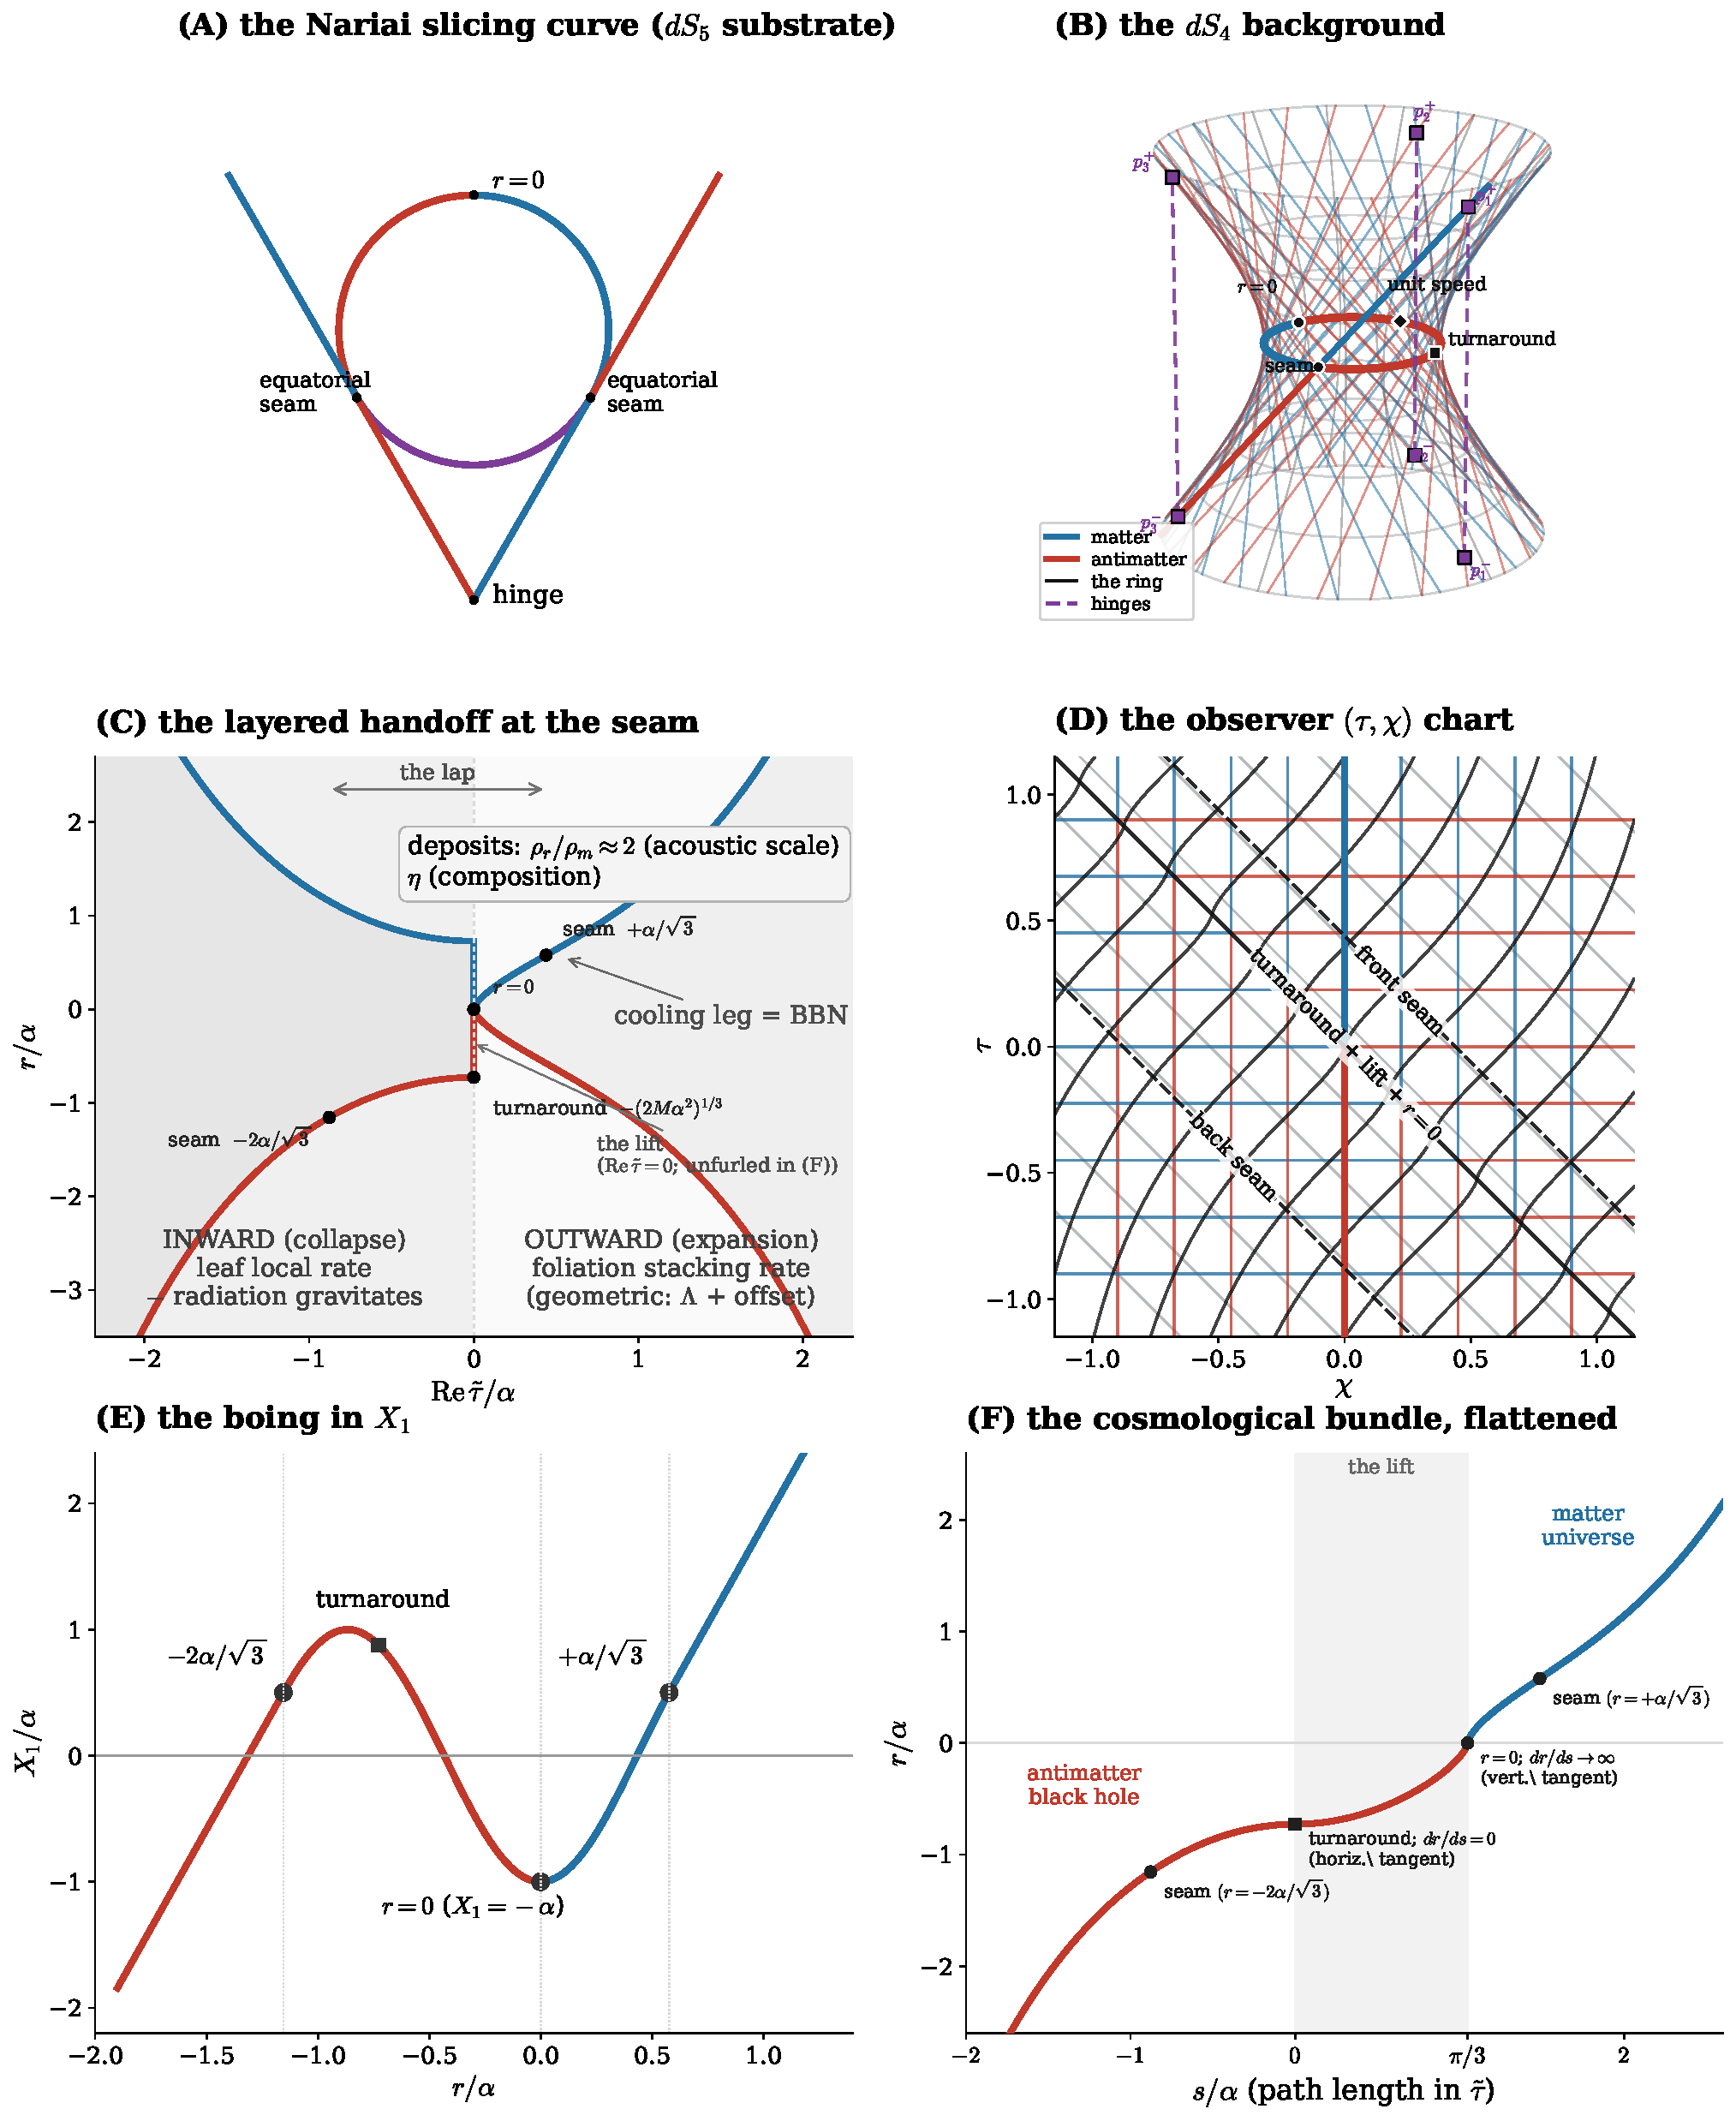
\includegraphics[width=\textwidth]{dS-SdS-synthesis.pdf}
    \caption{\textbf{The cosmogenetic bead, in six panels.} \emph{Colour code:} blue $=$ matter ($r>0$), red $=$ antimatter ($r<0$), the two exchanged at the branch point $r=0$. Where both $R$-conjugate null frames are drawn together---the $A$ worldline congruence and its $B$ synchronous-space dual---they read in opposite senses, each matter (blue) on its own $r>0$ side. Purple marks where the two conjugate readings run together over the same arc carrying opposite species, so that both colours are laid on one curve---in panel \textbf{(A)}, the hinge-side third of the equator. Black $=$ the photon congruence (the at-rest worldlines / null geodesics); grey $=$ the $S^3$ layers (the universe). Where a panel draws none of these, its curves are neutral light grey.
\textbf{(A)}~The Nariai slicing curve, the cut of the $dS_5$ substrate, seen from overhead (North-pole projection), with both conjugate bundles drawn. Each bead swings in from the hinge along a ruling, meets the equator at its tangent point---the equatorial seam---wraps, and exits along the other ruling; the two ruling lines cross at the hinge. Each bead splits its wrap $120^\circ$ before its turn at $r=0$ and $240^\circ$ after, and the two beads turn at the same $r=0$: one carries its blue $120^\circ$ arc up the right of the equator and its red $240^\circ$ arc back around, the other its red $120^\circ$ arc up the left and its blue $240^\circ$ arc back. The two therefore agree in colour over the upper two thirds---blue on the right third, red on the left---and differ only on the hinge-side third, where the two $240^\circ$ arcs overlap carrying opposite species: that third is drawn purple.
\textbf{(B)}~The $dS_4$ background: the two null ruling bundles, reassigned and spun about the axis as the representative bundle that generates the one-sheeted hyperboloid, one thick representative bead drawn over it. The reassignment promotes one bundle to the fundamental timelike congruence; matter (blue, $r>0$) and antimatter (red, $r<0$) are the two ends of the standing $R$-conjugation, the conjugate bundle read in the opposite sense. The photon congruence (black) and the $S^3$ layers (grey) complete it.
\textbf{(C)}~The layered handoff at the seam: the signed areal radius $r$ against the real part of cosmic time. The two $R$-conjugate bead readings---the matter reading $r(\tilde\tau)$ and its mass-reflected dual $-r(\tilde\tau)$---cross at $r=0$, each changing colour there (one running red\,$\to$\,blue, its conjugate blue\,$\to$\,red). Each reading is the theorem's own continuation (Thm.~\ref{thm:bead}): outward, $r=(2M\alpha^2)^{1/3}\sinh^{2/3}(3\tilde\tau/2\alpha)$ on the real axis; inward, $r=-(2M\alpha^2)^{1/3}\cosh^{2/3}(3\operatorname{Re}\tilde\tau/2\alpha)$ with $\operatorname{Im}\tilde\tau$ held at $-\pi\alpha/3$; and between them, where the radicand is negative, $\operatorname{Re}\tilde\tau$ does not advance at all---so the lift from the comoving turnaround $r=-(2M\alpha^2)^{1/3}$ (square) up to $r=0$ collapses here onto the single vertical segment at $\operatorname{Re}\tilde\tau=0$, and is drawn out in \textbf{(F)}. Circles mark the slicing roots $\pm$; the square marks the comoving turnaround, which is a $1-f=0$ point and not a root of the slicing (Lemma~\ref{lem:twoturnings}). On both legs alike the two rates are the one decomposition $H_{\text{leaf}}^{2}=H_{\text{stack}}^{2}+H_0^{2}\Omega_r(1+z)^{4}$ (Eq.~\ref{eq:two-rate}): content processes---the cooling leg's nucleosynthesis, the plasma's sound horizon and diffusion---run on the leaf's rate, where radiation gravitates, and comoving separations read across leaves run on the stacking rate, which the vacuum kernel fixes from $\Lambda$ and the cut's offset alone, radiation being a bend of the cut and no part of it; the $S^3$ layers (grey) pile onto the branch point, depositing $\rho_r/\rho_m\approx2$ (the acoustic scale) and $\eta$ (composition).
\textbf{(D)}~The observer's proper $(\tau,\chi)$ chart---panel \textbf{(B)} flattened. The $A$ congruence appears as the constant-$\chi$ worldlines (blue above the seam, red below); the $B$ congruence as the flat synchronous space (constant $\tau$, its conjugate dual, read in the opposite sense---red on the $r>0$ side, blue on the $r<0$); the photons as the null geodesics (black) crossing the branch point $\tilde\tau=\tau+\chi=0$ (the locus $r=0$, the diagonal $\tau=-\chi$) into the collapse side; the $S^3$ layers as the constant-$r$ diagonals (grey).
\textbf{(E)}~The boing in $X_1$---the geometry $r$ traces, of which \textbf{(F)} is the cosmic-time reading. $X_1=-\alpha\cos(2\pi r/\sqrt3\,\alpha)$ on the lap, through the roots $+\alpha/\sqrt3$, $0$, $-2\alpha/\sqrt3$ (trough $X_1=-\alpha$ at $r=0$), running straight on the ruling legs, in from and out to infinity; in the phase $\varphi=2\pi r/\sqrt3\,\alpha$ the three roots sit at $\varphi=+2\pi/3$, $0$ and $-4\pi/3$---the clean $120^{\circ}/240^{\circ}$ split---while the comoving turnaround falls at $\varphi=-2\pi\sqrt[3]{2}/3\approx-151.2^{\circ}$, off the lattice by exactly the $\sqrt[3]{2}$ that is the other cubic's signature, so the turnaround cannot be read as a fourth root of this one; red for $r\le0$, blue for $r\ge0$. The roots are the turning points of the \emph{slicing} ($f=0$) and are marked with circles; the comoving turnaround $r=-(2M\alpha^2)^{1/3}$, where the \emph{cosmic-time} reading turns ($1-f=0$), is marked with a square---the two parametrisations turn at different radii (Lemma~\ref{lem:twoturnings}), and the square is on the curve without being a turning point of it.
\textbf{(F)}~The cosmological bundle, flattened: the single privileged worldline of \textbf{(A)} and \textbf{(B)}---the antimatter black hole collapsing (red, $r<0$) through $r=0$ and continuing as our matter universe (blue, $r>0$)---as \emph{one} 2-D curve, the signed areal radius $r$ against the arc length $s$ along the bead's path in complex cosmic time $\tilde\tau$ (collapse at $\operatorname{Im}\tilde\tau=-\pi\alpha/3$; the lift at $\operatorname{Re}\tilde\tau=0$, $\operatorname{Im}\tilde\tau$ running $-\pi\alpha/3\to0$; expansion at $\operatorname{Im}\tilde\tau=0$). Nothing is projected and no $r$ value flattened---only $\tilde\tau$'s phase---so the whole bead runs single-valued and monotonic from $-\infty$ to $+\infty$ and the two bends read directly: the comoving turnaround at $r=-\sqrt[3]{2}\,\alpha/\sqrt3$, where $dr/ds=0$ (a horizontal tangent, the collapse stops), and the branch point $r=0$, where $dr/ds\to\infty$ (a vertical tangent, the bounded non-barrier crossing of the second structural fact). The shaded band is the lift, the $\pi\alpha/3$ stretch of path where $\operatorname{Re}\tilde\tau$ does not advance, across which $r$ climbs from the turnaround through $r=0$; the two seams sit at $r=-2\alpha/\sqrt3$ and $r=+\alpha/\sqrt3$, the $120^\circ/240^\circ$ split of \textbf{(A)} reappearing as their $2{:}1$ spacing along $s$. Both bends are legible and nothing is hidden behind a viewing angle.\rcpt{F_flat}}
    \label{fig:dS_SdS}
\end{figure*}

Four-dimensional de~Sitter space \cite{deSitter1917} may be represented as a one-sheeted hyperboloid embedded in five-dimensional Minkowski space, and its null geodesics are straight null lines of the embedding that lie on the hyperboloid (each spanned, with the origin, by a null $2$-plane). In the CR framework a single future-directed congruence of these null lines plays the structural role: the family whose causal sense matches the event-horizon generators arising during gravitational collapse. This bundle of future-directed null curves on the de~Sitter hyperboloid is the one reassigned to timelike to define the fundamental congruence in the Schwarzschild--de~Sitter (SdS) projection.

The complementary congruence used in the reassignment is \emph{not} another family of null lines. Instead, it is the congruence of \emph{at-rest comoving worldlines}---those that remain fixed on the expanding 3-spheres, each at a fixed point of the $3$-sphere with $3$-sphere radius $X=\alpha\cosh(T/\alpha)$ growing as the slices expand. These are the closed-slicing comoving geodesics, \emph{timelike} in de~Sitter space, but in the SdS projection they are reinterpreted as null geodesics and serve as the photon congruence. This exchange of causal roles---the two congruences trading their timelike and null characters, the null rulings becoming timelike and the timelike at-rest worldlines becoming null---is an instance of the representational freedom of \S\ref{sec:reassignment}, where distinct Lorentzian metrics on the same manifold encode different causal assignments while preserving the underlying foliation. Thus the causal reassignment proceeds as follows:
\begin{itemize}
    \item The future-directed null generators associated with the collapse-induced horizon structure are reinterpreted as the \emph{timelike} worldlines of fundamental observers.
    \item The at-rest comoving worldlines, which trace points that remain at fixed locations on each 3-sphere (the closed-slicing comoving geodesics, \emph{timelike} in de~Sitter), are reinterpreted as the \emph{null} trajectories of photons.
\end{itemize}

This reassignment preserves the foliation by evolving 3-spheres while altering the causal roles of the two congruences. The resulting projection remains fully diffeomorphism invariant and yields the Schwarzschild--de~Sitter spacetime as the unique vacuum representation compatible with the reassigned causal structure. The geometric structure underlying this reassignment is illustrated in Fig.~\ref{fig:dS_SdS}.

\subsection{Construction of the Schwarzschild--de~Sitter Representation}

To represent this causal reinterpretation, we take the radius of the expanding 3-sphere as a timelike coordinate $r$. Since each spatial slice is a 3-sphere orthogonal to $r$, the remaining spatial dimensions are spherically symmetric. A general line element consistent with these conditions takes the form
\begin{equation}
    \mathrm{d}s^2=-B(r,t)\,\mathrm{d}r^2
    +A(r,t)\,\mathrm{d}t^2+r^2\,\mathrm{d}\Omega^2.
\end{equation}

Imposing the vacuum Einstein equations with a positive cosmological constant selects the Schwarzschild--de~Sitter (SdS) metric \cite{Kottler1918}:
\begin{equation}
    \mathrm{d}s^2
    =-\frac{r}{\frac{\Lambda}{3}r^3+\frac{2GM}{c^2}-r}\,\mathrm{d}r^2
    +\frac{\frac{\Lambda}{3}r^3+\frac{2GM}{c^2}-r}{r}\,\mathrm{d}t^2
    +r^2\mathrm{d}\Omega^2.
    \label{eq:SdS-static}
\end{equation}
The coordinate $r$ is timelike when
\begin{equation}
    \frac{\Lambda G^2 M^2}{c^4}\geq\frac{1}{9},
    \label{eq:SdS-cosmology-condition}
\end{equation}
with the boundary value
\begin{equation}
    \frac{\Lambda G^2 M^2}{c^4}=\frac{1}{9}
    \label{eq:Nariai-condition}
\end{equation}
defining the \emph{Nariai configuration}, at which the two positive roots of the metric function coincide, at $r_{N}=1/\sqrt{\Lambda}$, and the mass is fixed to
\begin{equation}
    M=\frac{c^2}{3\sqrt{\Lambda}\,G}.
    \label{eq:Nariai-mass}
\end{equation}

The cosmological reassignment selects this boundary case, and the selection is geometric rather than a tuning\rcpt{P07_nariai_selection}. The de~Sitter hyperboloid is ruled by null generators; the reassignment promotes one such bundle to the fundamental timelike congruence (Fig.~\ref{fig:dS_SdS}). A comoving worldline of this congruence runs along a null generator of the embedding, and it is the only worldline of the SdS family that encounters no horizon along its length: every configuration with $\Lambda G^2M^2/c^4<1/9$ has its fundamental curve cross the embedding's symmetry structure transversally, and that transverse crossing is precisely what produces the finite-mass black-hole and cosmological horizons of a localized source. Only the Nariai tilt---the self-dual null direction at which the two positive horizons merge---gives a comoving curve that produces no such horizon, and so only the Nariai configuration admits a reading as a cosmology rather than as the field of a localized mass. The cosmology is therefore not one member of an overcritical family selected by fitting a mass; it is the unique non-pivoting member, fixed by $\Lambda$ alone. The geometric construction underlying this selection---in which the SdS horizons are the turning points of a single radial slicing curve and Nariai is the fixed point of that curve's root-exchange involution, the configuration of maximal mass any slicing of a given de~Sitter geometry can carry---is developed in the companion paper \cite{JanzenSlicing}, and the same uniqueness is obtained algebraically in the description groupoid: the generic vantages fall into two-cycles of that involution and Nariai is its one fixed point, so the reassignment---forbidden by the two-cycle structure at every generic vantage---selects it and no other, a structural fact about the groupoid rather than a fitting \cite{JanzenGroupoid}. Here we take the Nariai configuration as the cosmological case the reassignment picks out and read off its consequences.

This selection is not merely internal to the reassignment; it is forced by the limiting causal structure of gravitational collapse. The companion causality paper establishes that the future event horizon $\mathcal{H}^+=\partial J^-(\mathscr{I}^+)$ is approached by every exterior-adapted slicing only in the limit of infinite exterior time, the slices becoming \emph{asymptotically tangent} to a single horizon generator and meeting $\mathcal{H}^+$ at no finite time \cite{JanzenBHcausality}. The limiting orientation the collapse selects is therefore a null direction \emph{grazing} the horizon---tangent to it, never transverse. Promoting that direction to the fundamental timelike congruence, as the reassignment does, and classifying the family by how a null-generator congruence meets the horizon, yields a trichotomy: transverse crossing ($\Lambda G^2M^2/c^4<1/9$, two distinct positive horizons), tangency at a merged double root ($\Lambda G^2M^2/c^4=1/9$, \eqref{eq:Nariai-condition}), or no real horizon ($\Lambda G^2M^2/c^4>1/9$). A collapse forms a horizon, excluding the horizonless overcritical case; the limiting orientation is tangent rather than transverse\ldg{figure_theorem}, excluding the undercritical case; and the unique member whose null-generator direction is tangent to its horizon is the Nariai configuration, the self-dual direction at the merged root. The asymptotic alignment of collapse therefore forces the Nariai member. This supplies the identification deferred in \cite{JanzenBHcausality}, where the null direction the horizon selects is promoted to the fundamental congruence and the external universe is named the unique non-pivoting (Nariai) member: that promotion is here shown to be not merely admissible but selected by the limiting structure of the horizon the cosmology continues.

The forcing fixes the Nariai \emph{member}---the self-dual null direction, the double root---and what is metrically true at the seam follows from the double root itself. At Nariai the two positive roots of the horizon cubic \emph{merge}: the black-hole horizon and the cosmological horizon coincide, both at the areal radius $r_{N}=\alpha/\sqrt3$, with equal areas $4\pi\alpha^2/3$. (This is the $M>0$ member of a parity-conjugate pair. The three horizon roots sum to zero, so they cannot share a sign: for $2M>0$ two are positive and one negative, and for $2M<0$ one positive and two negative---two critical Nariai configurations, at $r_0^2=1/3$ and $r_0^2=4/3$, exchanged by the backward-radial reflection $r\mapsto-r$ that reverses the mass. The cosmology selects the $M>0$ member; the full root structure and its fundamental ellipse $r^2+rr_0+r_0^2=1$ are developed in the companion papers~\cite{JanzenSlicing,JanzenGroupoid}.) At the occurrence the two horizons are therefore one, and the null-boundary correspondence between them is \emph{metric} there---the identity on a single coincident horizon---not merely causal. This corrects a reading on which the two are held metrically apart. The areas $16\pi G^2M^2/c^4$ and $4\pi\alpha^2$ that differ are the family's two \emph{limits}---the Schwarzschild ($\Lambda\to0$, horizon $2GM/c^2$) and the empty de~Sitter ($M\to0$, horizon $\alpha$)---and equivalently the generic pre-seam correspondence, in which the collapsing horizon is still small and the cosmological horizon large and the two are mapped causally; neither is the seam, where the configuration is Nariai and the horizons are one. What the forcing does \emph{not} give is the identity $r_{N}=\alpha$, nor $\alpha$ as an output of the collapse: the merged seam horizon sits at $\alpha/\sqrt3$, a fixed fraction of the de~Sitter scale, and $\alpha=\sqrt{3/\Lambda}$ is fixed by $\Lambda$ alone. The de~Sitter scale $\alpha$ is the \emph{size} of the throat $3$-sphere, a distinct quantity from the areal radius $\alpha/\sqrt3$ of the merged horizon carried on it---conflating the two is the crossing this paragraph is at pains to prevent. The forcing determines which member of the family occurs, and that at the occurrence the two horizons coincide; it does not set the value of the invariant.

The locus $r=0$ in Eq.~\eqref{eq:SdS-static} is a genuine curvature singularity for the massive\rcpt{P07_sds_kretschmann} ($M\neq0$) Nariai configuration: the Kretschmann scalar diverges as $48G^2M^2/c^4r^6$ there. Consistent with the companion papers~\cite{JanzenBHcausality,JanzenCircle}, it is a real metric singularity, not a coordinate artefact; what the causal reassignment alters is the causal role of the congruences threading the geometry, not the reality of the singularity. This construction exemplifies how a change of metric on a fixed manifold, subject to compatibility with the underlying foliation, produces a distinct but admissible Lorentzian representation of the same ontological evolution.

\subsection{Fundamental Observers and the Induced Metric}

Fundamental observers correspond to worldlines comoving with the spatial 3-spheres of constant $r$ (fixed $\chi,\theta,\phi$); on account of the non-synchrony these are orthogonal to the constant-$\tau$ rest-frame slices rather than to the constant-$r$ slices themselves. In their proper frame, the line element becomes \cite{Janzen2015}
\begin{equation}
    \mathrm{d}s^2=-\mathrm{d}\tau^2
    +(\partial_{\chi} r)^2\mathrm{d}\chi^2
    +r^2\mathrm{d}\Omega^2,
    \label{eq:SdS-fundamental}
\end{equation}
where
\begin{equation}
    r(\tau,\chi)
    =\left(\frac{6GM}{\Lambda c^2}\right)^{1/3}
    \sinh^{2/3}\!\left(
        \frac{3}{2}\sqrt{\frac{\Lambda c^2}{3}}\,(\tau+\chi)
    \right),
    \label{eq:r-SdS-solution}
\end{equation}
defined on $\tau+\chi>0$.

The quantity $\tilde{\tau}=\tau+\chi$ defines the parameter along which the 3-sphere radius evolves. Since this parameter is tilted relative to the fundamental rest frame, the universe is \emph{non-synchronous}: spatial slices of constant $\tau$ are Euclidean but do not coincide with cosmological spatial slices.

\subsection{What this cosmology opens onto}

The framework laid out in this paper---the layered ontology, the projection principle, and the causal reassignment that selects the Nariai member---finds its final application in a complete physical cosmology, of which the construction to this point fixes the geometric core: the proper-frame line element~\eqref{eq:SdS-fundamental} carries the exact $\sinh^{2/3}$ law~\eqref{eq:r-SdS-solution} of flat $\Lambda$CDM, and the Null--Boundary Correspondence proved below (\S\ref{sec:null-boundary-correspondence}) fixes that cosmological future at the collapse horizon. The physical theory this determines is developed in full across the companion arc; we describe it here, as the synthesis the framework culminates in, with the forward references that make that synthesis coherent. The descriptions that follow deliberately overlap the companion papers---each develops formally what is synthesised here---because the theory is one, and is read off a single $\Lambda$-set de~Sitter geometry.

\emph{The expansion history and the contents.} The areal radius~\eqref{eq:r-SdS-solution} is not merely \emph{like} the flat-$\Lambda$CDM scale factor; at the Nariai member it \emph{is} that scale factor, with both the rate $\tfrac12\sqrt{3\Lambda}\,c$ and the amplitude---a length set by $\Lambda$ alone, distinct from the de~Sitter $3$-sphere size $\alpha=\sqrt{3/\Lambda}$ and from the merged-horizon areal radius $\alpha/\sqrt3$---fixed by the cosmological constant, with no parameter left to tune. The Friedmann densities are then bookkeeping for one $\Lambda$-set geometry rather than its drivers: the matter fraction is not an independent amplitude but the reading of a clock, so that the present value $\Omega_{m,0}$ records the cosmic epoch $\tilde\tau_0$ at which we observe, and the so-called coincidence problem dissolves into the observation that we exist at a time of order the single timescale the geometry possesses, $\sim\!1/(\sqrt\Lambda\,c)$. The expansion law, the density bookkeeping, and the dissolution of the apparent Hubble and acoustic tensions are developed in full in the companion cosmology paper~\cite{JanzenCRcosmology}, which carries the cosmology through to the microwave background; the early-universe divergence from standard $\Lambda$CDM is treated below (\S\ref{sec:null-boundary-correspondence}).

\emph{The tensions, dissolved.} Because radiation carries no term in the rate at any epoch, the two frameworks part before recombination, and the apparent tensions of the standard model become consequences of that one structural fact rather than puzzles to be fitted. There is no second Hubble rate to reconcile: the directly measured $H_0$ is the geometry read at the present epoch, while the lower value inferred from the microwave background rests on a radiation-governed sound horizon the construction does not share, so the Hubble tension dissolves. The acoustic scale is then met at the directly measured rate by a single inherited datum (\S\ref{sec:inherited-datum})---the radiation amplitude at the branch point, $\rho_r/\rho_m\approx2$, a measured matter content and the structural analogue of the baryon-to-photon ratio that flat $\Lambda$CDM itself carries from outside its own model. \emph{The fitted quantity is the onset redshift and it does not move with $H_0$ at all}---which is what makes it a datum rather than a knob for the tension---\emph{while the ratio is that redshift re-expressed in units of a physical matter density the construction does not itself determine, and is accordingly an order-unity band ($1.7$--$2.0$ across the Hubble range) rather than a determined number}~\cite{JanzenCRcosmology}. This resolution is developed in full in the companion cosmology paper~\cite{JanzenCRcosmology} and carried into its microwave-background sector; we synthesise it here as one consequence of the geometric rate. The same handover fixes the light-element composition, produced on the cooling leg by a genuine nuclear network: helium-4, helium-3 and deuterium at their observed values (deuterium and helium-4 within $1\sigma$ of the measured primordial values), the near-zero metallicity of the oldest systems from the handover, and lithium-7 carrying the standard threefold over-prediction---the lithium problem shared with flat $\Lambda$CDM rather than dissolved, the cooling leg being a standard nucleosynthesis---all developed in the cosmogenesis paper~\cite{JanzenCosmogenesis}.

\emph{The recovered cosmic time.} The same non-orthogonal foliation the reassignment installs resolves the canonical problem of time. With the cosmic clock supplied by the existent---the comoving congruence whose rest frame the redshift isotropy measures~\cite{JanzenModernParallax}---rather than by the bare geometry, the scalar constraint deparametrizes to a true Hamiltonian generating the layers' advance, and the frozen Wheeler--DeWitt dynamics stand revealed as the symptom of granting the four-manifold an existence the layered ontology withholds. The objective cosmic ``now'' and the relativity of synchrony are thereby reconciled rather than opposed (\S\ref{sec:CR-axioms}); the canonical structure is developed in the companion canonical-time paper~\cite{JanzenCanonicalTime}.

\emph{The matter dynamics.} What sets a given epoch's contents is the bend of the spatial cut: the matter density is the cut's deviation from the empty-de~Sitter slicing, forced by the same empirical foliation that forces the rate, not by a separate dynamical input~\cite{JanzenModernParallax}. The dynamics of that bend---the slicing operator whose generative boundary is the wall at which free gravitational radiation switches on, and the chiral matter the seam continuation carries onto the cosmological side---are the subject of the dynamics paper~\cite{JanzenDynamics} and its operator and range companions~\cite{JanzenOperator,JanzenRange}. In the linear regime the leaf's transverse-traceless shear is the gravitational wave (\S\ref{sec:CR-applications}), returning the standard graviton as the projection-dependent representation of a spatial-metric perturbation.

\emph{The perturbation spectrum.} Finally, the de~Sitter substrate fixes the \emph{structure} of the primordial spectrum while the progenitor handover supplies its \emph{content}. The sharp acoustic coherence is itself substrate-fixed---the null boundary sets one phase per mode, the common phase computed to yield the regular comb that randomized phases wash out, where the sub-horizon seam admits no super-horizon freeze-out---and the source spectrum is that of a closed $S^3$, discrete by degree, but projected to the sky through the \emph{flat} distance slicing rather than a closed one---the flat/closed decoupling carried by the non-synchrony. The flat projection of the discrete source leaves a parameter-free low-multipole \emph{deficit}: the lowest physical mode, fixed by $\Lambda$ through the present curvature radius, lands near $\ell\approx8$ with no power below it. On a genuine Boltzmann transfer the deficit is mild and shaped---a dip bottoming at $\ell=4$ ($\approx0.47$, $0.41$, $0.36$, $0.68$ of the expectation at $\ell=2,3,4,5$), its shape cross-validated between two independent transfers---and non-discriminating, consistent with the standard model within the lowest multipoles' cosmic variance; the confrontation is developed in the cosmology paper. The degenerate cosmological-horizon seam, in turn, transmits the inherited content faithfully rather than imprinting a scale of its own. The decomposition of the observed spectrum into substrate-fixed structure and handover-fixed content, and its consequences for the microwave background, is the work of the cosmology paper~\cite{JanzenCRcosmology}, which opens with the cosmological theory synthesised here and closes it by developing that sector.

\emph{The economy of assumption.} Read as one theory, this cosmology reaches the observations the standard model reaches, and the substance of the comparison is what each must assume to do so. The standard model \emph{assembles} the observed universe---a dark-energy component for the acceleration~\cite{Riess1998,Perlmutter1999}, an inflationary sector for the causal contact, flatness, coherence, and near-scale-invariance its background dynamics do not supply, added early-universe physics where the sound horizon and the rate come into tension---a dedicated part per phenomenon. This construction adds none: those same phenomena are read off structure the single $\Lambda$-set geometry already carries---the isotropizing throat, the coherence-fixing null boundary, the exactly Euclidean slice, the degenerate horizon that transmits rather than imprints---each fixed by $\Lambda$ alone, with no parameter free to produce it. That is the distinction between a structure that \emph{requires} a phenomenon and one that merely \emph{permits} it through adjustable apparatus---the criterion by which competing frameworks are rightly weighed ahead of the measurement that will decide between them~\cite{JanzenShadowExistence}, the same the programme applies in reading the cosmic foliation as forced rather than chosen~\cite{JanzenModernParallax}. Drawn in full in the cosmology paper~\cite{JanzenCRcosmology}, that reckoning falls to this construction on the theory-choice axis now---and the data axis has begun to move with it. The geometric rate resolves the Hubble tension across the acoustic scale and the baryon-acoustic distance ladder together, at the directly measured $H_0$ where the standard model cannot~\cite{JanzenCRcosmology}; and the forced cooling leg produces the light-element abundances, deuterium and helium-4 within $1\sigma$ of the measured primordial values~\cite{JanzenCosmogenesis}. So two of the discriminators once owed are returned in this construction's favour---a data result, not a tie, and on the baryon-acoustic ladder now confirmed against the state-of-the-art DESI~DR2 dataset at $\chi^2/\text{dof}\simeq1$---with the low-multipole comparison now a mild deficit consistent with the standard model within cosmic variance, and the $8.2\%$ damping-\emph{scale} signature a computed, non-reabsorbable CR-specific effect whose observable consequence awaits the full high-$\ell$ acoustic transfer, genuinely open. And the reading makes falsifiable commitments---no inflationary scale-invariant attractor, no consistency relation, no substrate-sourced primordial $B$-modes---exactly where the standard picture keeps its freedom.

These developments are not appendices to the construction but its point. The layered ontology was introduced to render the observed universe intelligible, and the cosmology, the dissolved tensions, the recovered cosmic time, the matter dynamics, and the perturbation spectrum are the one physical theory it determines---each a face of a single $\Lambda$-set de~Sitter geometry read through the reassigned causal structure. The geometric result this paper proves is that theory's foundation; the companion arc is its development; the observed universe is its Nariai reading.

\subsection{The inherited datum}\label{sec:inherited-datum}

\emph{Inherited boundary data, derived rather than measured.} The acoustic scale is met at the directly measured $H_0$ by a single inherited datum, the branch-point radiation amplitude $\rho_r/\rho_m\approx2$ (the structural analogue of the baryon-to-photon ratio), so it stands as a one-parameter accommodation rather than a parameter-free prediction. \emph{The datum proper is the onset redshift, which is $H_0$-independent; the ratio is its restatement in an imported density, so what a derivation must land is an order-unity number in the band $1.7$--$2.0$ and not the figure two to two places.} The open work is the baryogenesis-analogue derivation of the progenitor handover---the composition, and the primordial amplitude and tilt $A_s,n_s$~\cite{JanzenCRcosmology}---with the consistency target the measured primordial abundances (deuterium, the helium-4 fraction, the near-zero metallicity of the oldest systems). The composition half of that target is carried in the cosmogenesis paper~\cite{JanzenCosmogenesis}: the progenitor handover heats the infalling matter above the deuterium bottleneck and re-expands through it at the standard rate, so the cooling leg is a standard nucleosynthesis that \emph{produces} helium-4 and deuterium at their observed values and shares the standard lithium problem---the light-element consistency target met, the derivation of the single inherited datum remaining the open work. Like $\eta$, the datum may remain empirical at no cost to the dissolution; deriving it is the eager target.

\emph{The frontier is two data and not one, and the papers should be read together on this.} The handover
supplies the radiation amplitude $\rho_r/\rho_m$, which fixes the acoustic \emph{spacing} and is the datum the
one-parameter accommodation turns on; and it supplies the baryon-to-photon ratio $\eta$, which fixes the
light-element abundances and the acoustic peak \emph{heights}~\cite{JanzenCosmogenesis}. \emph{These are not, on inspection, distinct data}, and the correction runs in the
construction's favour. Given $\eta$ and the measured matter-to-baryon ratio, the radiation amplitude at
onset is fixed by the onset temperature alone---$\rho_r/\rho_m=[1+\nu](\pi^4/30\zeta_3)T_{\mathrm{onset}}
/[\eta\,(\omega_m/\omega_b)m_N]$, returning $1.99$ at $T_{\mathrm{onset}}=1.6\,$eV, which is the quoted
value to one per cent from standard thermodynamics and nothing else. \emph{So the ``single inherited
datum'' of the acoustic-scale statement above is the fitted onset restated, not a number standing beside
$\eta$}: what the handover supplies is one composition datum, and what the cosmology fits is one
parameter~\cite{JanzenCRcosmology}. The composition half of the consistency target is met with $\eta$
inherited, exactly as flat $\Lambda$CDM inherits it; \emph{what the eager target asks is a derivation of
$\eta$ and of the onset}. \emph{And a derivation of $\eta$ is constrained in kind, not merely in difficulty.} The cosmogenesis account has the infall thermalize four orders above the deuterium bottleneck, so the progenitor's composition is erased and the abundances are synthesized in the window rather than inherited; what survives that passage is baryon number, which no dissociation destroys, and $\eta$ is a ratio of baryon number to photon number~\cite{JanzenCosmogenesis}. \emph{So $\eta$ is inherited because it is protected by a conservation law, and the abundances are predicted because they are not.} \emph{A derivation of $\eta$ must therefore reach a conserved charge of the progenitor}, and can draw on nothing the peak erases---which excludes the entire nuclear history and leaves the baryon asymmetry itself as what would have to be explained.

\emph{The discrete side of that frontier stands across three papers.} The skeleton the programme reads off the horizon cubic is $\mathrm{Aut}(A_2)$, of order twelve. The residue pairing which the
horizon roots' surface gravities place on the root triple has a holonomy about the Nariai points---a Klein
four-group, arising as the per-root resolution of the same $\sqrt{\Delta}$ whose non-squareness fixes the Galois
group---and adjoining it closes the Weyl group of $\so(6,\mathbb{C})$, the complexification of the substrate's
own isometry algebra~\cite{JanzenGroupoid, JanzenAlgebroid}. \emph{So the sector's discrete group is the
substrate's own}, and what was being used is the sub-root-system obtained by reading only the cubic.

\emph{Two consequences bear on this section's accounting.} The generation count acquires a protection it did not
have: the holonomy changes the walls' chiralities only in pairs, so $\dim\ker_-$ cannot be reached from
$\dim\ker_+=3$ by any number of loops, and the observed uniform-chirality configuration is the unique member of
its orbit~\cite{JanzenMatter}. And the continuous question is closed on both real forms rather than one: the
substrate's canonical connection is genuinely non-abelian, with holonomy in $\so(4,1)$, and neither $\su(3)$ nor
$\mathfrak{su}(2,1)$ embeds---on the tangent bundle because both require six real dimensions where five are
available, and on the spinor bundle because a compact algebra of dimension eight cannot sit in a group whose
maximal compact is six-dimensional---\emph{that six being the fixed-point set of $\so(4,1)$'s Cartan
involution $\theta(X)=\eta X\eta$, which is what a maximal compact subalgebra
is}\rcpt{I1_so6C_has_five_real_forms_and_the_omitted_one_admits_su3}---while the non-compact form
founders on the quaternionic structure
$\mathfrak{sp}(1,1)$ preserves. \emph{The wall reported in the boundary paper is therefore not particular to the
compact form}, and the frontier's continuous half stands where that paper places it. \emph{And the two are not free of one another, though the relation between them is not a further datum.}
They are quantities of different kinds: $\rho_r/\rho_m$ is a ratio of \emph{energy densities} taken over the
matter as a whole, while $\eta$ is a ratio of \emph{numbers} taken over the baryons alone. \emph{Passing between
them requires knowing what the matter is}---which fermions the handover delivers, in what numbers, and at what
masses. That the two are not the same quantity is not a modelling choice but a fact about the world: matter is
not baryons, a neutral hydrogen plasma carrying one electron for every proton, so a count by baryon number
omits half its particles.

\emph{So the composition frontier and the fermion-sector frontier are one frontier read at two ends.} The
matter sector supplies the number of generations, their chirality and the family symmetry relating them, and
declares the representation content---which species, in which multiplets, with which masses---not
delivered~\cite{JanzenMatter, JanzenBoundary}. \emph{That undelivered content is exactly what stands between the
two composition data.} A derivation of either therefore waits on the same thing, and the appearance of two
independent empirical inputs is the appearance the missing sector presents from the cosmological side.
\emph{We claim no derivation here and record only the identification}: the target of this item and the
unbuilt route of the matter sector are not separate debts.  \emph{Two constraints on that derivation are now established, and both narrow it rather than advance it.}
The first fixes the \emph{class} of what can be inherited: the segment preceding the branch point acts on
perturbations as a filter that damps oscillatory content and leaves frozen content untouched, and every mode
has exited the shrinking comoving horizon before the crossing, so what crosses is non-oscillatory---an amplitude
and a tilt, never a phase (\S\ref{sec:lift-quantum}). \emph{The scope of that constraint should be stated exactly.} It is an argument about perturbation modes, so it binds the primordial amplitude and tilt: $A_s$ and $n_s$ are of the frozen class, and a candidate derivation producing a phase-carrying primordial datum is excluded on that ground alone. \emph{It does not bind the composition}: $\rho_r/\rho_m$ is a background ratio, not a mode, and the filter argument says nothing about it. \emph{So the frontier's two halves are constrained differently}---the spectrum's by the crossing's selection rule, the composition's not at all by it---and a derivation of the composition must be sought on other grounds.

The second excludes the mechanism one would try first. \emph{The crossing itself cannot supply an asymmetry}:
the imaginary segment's action has integrand $r[f(r)-1]=-2M-r^{3}/\alpha^{2}$, odd under the standing
conjugation acting on offset and mass together, so the two branches carry equal and opposite action summing to
zero identically~\cite{JanzenCosmogenesis}. \emph{The balance is exact and is traced to the same oddness that
fixes the chirality parity and the progenitor's antimatter identity}, so it cannot be lifted by refining the
crossing---what would have to fail is the relation that makes the progenitor antimatter at all. Whatever
supplies the datum must therefore be carried by the matter field or be genuinely inherited as content, and not
produced by the geometry of the handover. \emph{Neither constraint is a step toward the derivation}; together
they remove the most natural place to look and fix the shape an admissible answer can take.
%  REGISTER NOTE: the inherited datum was P7's frontier item 1 and register row `PO-16`; the row is
%  STRUCK -- the item is worked, and deriving the datum is a bonus rather than a debt -- so it no longer
%  stands in the frontiers list and lives here instead, as this section.

\section{Null--Boundary Correspondence and SdS Entry Geometry}
\label{sec:null-boundary-correspondence}

In Cosmological Relativity (CR), the ontological structure of the universe is encoded in a layered family of spatial manifolds
\[
\mathcal{U}=\{\mathcal{S}_t \mid t\in\mathbb{R}\},
\]
while Lorentzian spacetime metrics $(M,g)$ arise as representational projections of this evolving geometry. The causal structure of such projections may vary, provided the layered ontology and its cosmic foliation remain fixed. This freedom permits distinct spacetime metrics---including Schwarzschild, de~Sitter, and Schwarzschild--de~Sitter (SdS)---to represent the same underlying geometry through different causal assignments, as shown in the SdS construction above.

The purpose of this section is to establish a structural correspondence between two geometric objects:
\begin{enumerate}
    \item a null hypersurface arising as the limit of infalling timelike worldlines in a Lorentzian projection of CR, and
    \item the initial representational slice of an SdS cosmology obtained by causal reassignment.
\end{enumerate}

This correspondence is structural: it identifies a morphism between two projections of the same ontological layer. The theorem proved below establishes that the horizon event-of-events at the limit of collapse and the initial slice of an SdS cosmology represent the same ontological layer of CR under distinct causal assignments. What this identification implies for the post-horizon evolution---the dynamics on the cosmological side of the correspondence---is fixed by the SdS construction itself, whose expansion law is $\sinh^{2/3}$ as derived above; the transition of matter and observers across the branch point is not addressed in this section but is settled in \S\ref{sec:frontiers}, where the worldline side is computed: a comoving worldline reaches the branch point at finite proper time with divergent curvature and divergent tidal stretch and terminates there, what continues being the analytic continuation.  What \emph{is} settled about crossing concerns perturbation content rather than bodies: the cosmology paper gives a transmission mechanism at the branch point, on which the amplitude and tilt of a frozen mode cross unaltered while its oscillatory content does not~\cite{JanzenCRcosmology}.

\subsection{Horizon Null Structure and One-Way Causal Ordering}

Let $(M,g)$ be a Lorentzian manifold representing a gravitational collapse scenario. From the metric-singularity structure established in Ref.~\cite{JanzenBHcausality}, the event horizon $\mathcal{H}^+$ is a null hypersurface foliated by null generators $\gamma_\lambda$, where:
\begin{enumerate}
    \item each generator consists of topologically distinct, causally ordered, but metrically coincident events,
    \item successive infalling timelike worldlines accumulate asymptotically onto these generators, and
    \item the causal relation is one-way: earlier infalling worldlines lie in the past null boundary of later ones, but not conversely.
\end{enumerate}

Topologically, the horizon has the structure
\[
\mathcal{H}^+ \cong S^2 \times \mathbb{R}_{\ge 0},
\]
with $S^2$ the cross-sectional sphere and $\mathbb{R}_{\ge 0}$ parametrizing the null ordering along generators. This structure is what Theorem~\ref{thm:null-boundary} maps.

\subsection{SdS Cosmology and Causal Reassignment}

In the SdS construction above, we showed that by preserving the cosmic foliation while reassigning the causal roles of null and timelike congruences in de~Sitter space, one obtains a Schwarzschild--de~Sitter representation of the same layered ontology. The geometric legitimacy and structural meaning of this reassignment are clarified in the following subsection. In this construction:
\begin{equation}
    \mathrm{d}s^2
    = -\frac{r}{\frac{\Lambda}{3}r^3 + \frac{2GM}{c^2} - r}\,\mathrm{d}r^2
    + \frac{\frac{\Lambda}{3}r^3 + \frac{2GM}{c^2} - r}{r}\,\mathrm{d}t^2
    + r^2 \mathrm{d}\Omega^2,
\end{equation}
where $r$ is a timelike coordinate aligned with the cosmic foliation, and the spatial slices are 3-spheres of radius $r$.

In this representation:
\begin{enumerate}
    \item the fundamental cosmological rest frame is defined by one bundle of null generators of the de~Sitter hyperboloid;
    \item the complementary congruence becomes the null (photon) congruence in the SdS projection;
    \item the foliation by 3-spheres is preserved;
    \item the evolution of $r$ follows the $\sinh^{2/3}$ law matching flat $\Lambda$CDM.
\end{enumerate}

\subsection{Metric Reassignment and Representational Freedom on a Fixed Manifold}\label{sec:reassignment}

The causal reassignment employed in the SdS construction rests on a structural distinction that is standard in differential geometry yet rarely articulated in the relativistic literature. A smooth manifold $M$ is, by definition, a topological space equipped with a differentiable atlas; it carries no intrinsic geometric or causal structure. Lorentzian geometry arises only after the choice of a metric, that is, after specifying a smooth assignment to each tangent space $T_pM$ of a symmetric bilinear form of signature $(-,+,+,+)$. The null cones, causal relations, and classification of tangent directions as timelike, null, or spacelike are therefore features of the metric $g$, not of the manifold itself.

For a fixed Lorentzian metric $g$, the null directions at each point are invariant under coordinate transformations: changing charts cannot alter the light cone defined by $g$. However, there is no requirement that a given manifold admit only one such metric. Replacing $g$ with a distinct Lorentzian metric $g'$ on the same manifold $M$ alters the causal structure while leaving the underlying topology and differentiable structure unchanged. The pairs $(M,g)$ and $(M,g')$ thus represent the same manifold endowed with inequivalent Lorentzian geometries. This is entirely orthodox: the freedom to equip a single manifold with distinct Riemannian or Lorentzian metrics is foundational in differential geometry, and no part of the manifold structure is affected by such a replacement.

The causal reassignment carried out in this work is a highly constrained instance of this general freedom. Rather than introducing an arbitrary new metric, we consider two Lorentzian structures $g$ and $g'$ that share the same foliation by spacelike hypersurfaces corresponding to the layered ontology $\{\mathcal{S}_t\}$. The foliation is held fixed, while the causal classification of certain congruences threading this foliation is altered. Specifically, a congruence that is null with respect to $g$ may become timelike with respect to $g'$, and a congruence that is timelike in one representation may serve as the null (photon) congruence in another, provided the resulting $(M,g')$ retains smoothness and Lorentzian signature. In this sense, the SdS construction implements a reassignment of causal roles among congruences while preserving the manifold and the ontological layering.

This has a straightforward geometric reading. Altering the causal roles of congruences corresponds to selecting a different Lorentzian structure on the same underlying manifold, one that remains compatible with the same foliation. The transition from the de~Sitter metric to the SdS metric is such a selection: the manifold, its differentiable structure, and the ontological layering are held fixed, and only the metric assignment of null and timelike directions to the threading congruences is changed.

This perspective also clarifies the conceptual economy of the construction. The reassignment does not invoke higher dimensions, additional fields, or modifications of Einstein's equations. The manifold $M$ remains fixed; only the metric chosen to represent the causal structure is changed. From this viewpoint, the question addressed in the SdS construction is simply: given a manifold equipped with a fixed layered ontology, how many physically distinct Lorentzian metrics $g$ are compatible with that ontology and its cosmic foliation? More than one are admissible in general; the SdS metric arises as the choice selected by requiring compatibility with the horizon-induced temporal orientation identified in gravitational collapse, and the cosmological case among the SdS family is the Nariai configuration singled out above.

In this sense, a Lorentzian metric is equivalently understood as a choice of equivalence class of coordinate charts related by local Lorentz transformations, and replacing $g$ with $g'$ is a change of that equivalence class. The manifold itself is indifferent to which metric it carries; what changes is the causal projection of the underlying ontology that the metric encodes. The SdS cosmology therefore exemplifies how distinct Lorentzian representations of the same underlying manifold may encode different but admissible causal assignments, while preserving the ontological content encoded in the cosmic foliation.

\subsection{Null-Boundary Correspondence}

We now formalize the relationship between the null horizon structure and the SdS cosmic entry slice.

\begin{theorem}[Null-Boundary Correspondence in CR]
\label{thm:null-boundary}
Let $(M,g)$ be a Lorentzian projection of a CR ontology in which a null hypersurface $\mathcal{H}^+$ arises as the limit of infalling timelike worldlines. Let $(M',g')$ be an SdS representation of the same ontology obtained via causal reassignment while preserving the cosmic foliation.

Each comoving geodesic $p$ of the underlying de~Sitter background geometry---a point of the waist $3$-sphere of $\mathrm{dS}_4$---has an oriented future cosmological horizon $\mathcal{H}_c^{+}(p)$. In the static slicing adapted to $p$, in which $p$ is the worldline $r=0$ of
\[
ds^2 = -\Bigl(1-\tfrac{r^2}{\alpha^2}\Bigr)dt^2 + \Bigl(1-\tfrac{r^2}{\alpha^2}\Bigr)^{-1}dr^2 + r^2\,d\Omega^2,
\]
$\mathcal{H}_c^{+}(p)$ is the null hypersurface $r=\alpha=\sqrt{3/\Lambda}$ of the de~Sitter background geometry $(M,g)$, ruled by the generators that asymptote to but never meet $p$, with bifurcation $2$-sphere the equatorial $S^2$ of $p$ in the waist $3$-sphere; $\mathcal{H}_c^{+}(p)\cong S^2\times\mathbb{R}$.

Then there exists a correspondence
\[
\mathcal{N}:\mathcal{H}^+ \longrightarrow \mathcal{H}_c^{+}(p),
\]
\emph{canonically constrained} in that both are the oriented future horizon of a worldline---the collapse worldline on the left, $p$ on the right---so that $\mathcal{N}$ is fixed up to a reframing of the generator-labelling $2$-sphere, far from an arbitrary isomorphism of like-typed boundaries, by:
\begin{enumerate}
    \item $\mathcal{N}$ maps each collapse-horizon generator $\gamma_\lambda$ to a unique generator of $\mathcal{H}_c^{+}(p)$;
    \item the celestial $S^2$ cross-section of $\mathcal{H}^+$ maps onto the bifurcation $S^2$ of $\mathcal{H}_c^{+}(p)$, matching the observer-pole of each;
    \item the null affine ordering along the generators of $\mathcal{H}^+$ corresponds to that along the generators of $\mathcal{H}_c^{+}(p)$, with future orientation preserved;
    \item by Diffeomorphic Representability and the Non-Identity of Ontology and Representation, the layer represented along $\mathcal{H}^+$ and the layer represented along $\mathcal{H}_c^{+}(p)$ are one ontological layer: $\mathcal{H}^+$ and $\mathcal{H}_c^{+}(p)$ are distinct spacetime representations of the same existing 3-space.
\end{enumerate}
$\mathcal{N}$ preserves the null fibration, the affine ordering, and the future orientation, but is \emph{not} in general an isometry: the horizon areas ($16\pi G^2M^2/c^4$ for the collapse horizon, $4\pi\alpha^2$ for $\mathcal{H}_c^{+}(p)$) and the surface gravities differ. The identification is causal and structural, not metric. One residual freedom remains: $\mathcal{H}_c^{+}(p)$ carries a canonical labelling $2$-sphere (its bifurcation sphere, the boost fixed-point set), whereas the collapse horizon---not a bifurcate Killing horizon---carries no such distinguished cross-section, so the matching of generator labels in (ii) is fixed only up to a reframing of that $S^2$. The worldline role and future orientation thus constrain $\mathcal{N}$ to a single causal type, not to a unique map; this suffices for the correspondence, whose content is carried by the reassignment rather than by any metric identity.

The unequal areas and surface gravities here are those of the family's limiting members---the Schwarzschild ($\Lambda\to0$) collapse horizon, area $16\pi G^2M^2/c^4$, and the empty-de~Sitter ($M\to0$) cosmological horizon, area $4\pi\alpha^2$---and of the generic, pre-occurrence correspondence, in which the collapsing horizon is still small and the cosmological horizon large. At the occurrence itself the forced member is the Nariai double root (the alignment selection of \S\ref{sec:sds-cosmology}): there the two positive roots of the horizon cubic coincide, the collapse and cosmological horizons merge at the common areal radius $\alpha/\sqrt3$ with equal area $4\pi\alpha^2/3$, and $\mathcal{N}$ reduces to the identity on that single coincident horizon---metric at the seam. The causal-and-structural reading is the statement of the generic map; the seam is its metric coincidence, not a counterexample to it.

The residual labelling freedom is, in the same way, a feature of the generic map and not of the seam. It rests on $\mathcal{H}_c^{+}(p)$ being a \emph{non-degenerate} bifurcate Killing horizon---the de~Sitter horizon $r=\alpha$, surface gravity $1/\alpha\neq0$---whose bifurcation $2$-sphere, the boost fixed-point set, supplies the canonical labelling the collapse horizon lacks. At the occurrence the merged horizon is the Nariai double root, where $f=f'=0$ and the surface gravity vanishes: a degenerate horizon, which carries no bifurcation $2$-sphere (the bifurcation surface recedes in the degenerate limit). The canonical labelling sphere on which the reframing was defined therefore does not exist at the seam; with the two horizons coincident and $\mathcal{N}$ the identity on the single horizon, there are no longer two distinct cross-sections to reframe between, and the generic freedom does not carry over. At the seam $\mathcal{N}$ is thus metric \emph{and} rigid---the identity---whereas the reframing freedom is carried entirely by the generic, non-degenerate map. (Whether the single degenerate horizon retains a residual generator gauge of its own is a separate question of degenerate-horizon structure, immaterial to the present point: the asymmetry on which the reframing freedom was defined is absent at the seam.)

Moreover, the assignment $p\mapsto\mathcal{H}_c^{+}(p)$ is a \emph{bijection} between the comoving geodesics---the waist $3$-sphere, hence the full $S^3$ family filling the upper sheet---and the oriented future de~Sitter cosmological horizons. The de~Sitter-to-SdS reassignment of \S\ref{sec:CR-SdS} promotes, for each $p$, the generators of $\mathcal{H}_c^{+}(p)$ to the timelike worldline $p$; the $S^3$ of comoving worldlines that fills the upper sheet of $\mathrm{dS}_4$ with the $\sinh^{2/3}$ expansion is therefore the $S^3$ of reassigned horizons---no single horizon seeds the congruence, the family of horizons \emph{is} the congruence. The collapse horizon and the de~Sitter cosmological horizon are thus the null and timelike seams of one manifold under distinct causal assignments---inequivalent Lorentzian geometries representing the one ontological layer (\S\ref{sec:reassignment})---and the cosmological future is fixed at the event horizon: its causal structure is the horizon's null direction reassigned as non-orthogonal cosmic time, with the scale set by $\Lambda$. Concretely, it is the family $\{\mathcal{H}_c^{+}(p)\}$, each member the null counterpart under $\mathcal{N}$ of a collapse horizon, reassigned to the timelike congruence whose expanding $S^3$ slices are the SdS cosmology.
\end{theorem}

\begin{proof}
Both $\mathcal{H}^+$ and $\mathcal{H}_c^{+}(p)$ are oriented future null hypersurfaces of the structure $S^2\times\mathbb{R}$, and each is the future horizon \emph{of a worldline}: $\mathcal{H}^+$ is the future horizon of the collapse worldline, the limit onto which infalling timelike worldlines accumulate \cite{JanzenBHcausality}; $\mathcal{H}_c^{+}(p)$ is the future cosmological horizon of the comoving geodesic $p$, ruled by the de~Sitter generators that asymptote to but never meet $p$. This shared role---future-horizon-of-an-observer---constrains $\mathcal{N}$: the observer worldline on one side corresponds to $p$ on the other, the celestial $S^2$ of the collapse horizon to the bifurcation $S^2$ that is the equatorial $S^2$ of $p$, and the future-directed affine ordering to the future-directed affine ordering. $\mathcal{N}$ is therefore fixed to a single causal type---an oriented future-horizon-of-an-observer identification, far from one isomorphism among the many that any two $S^2\times\mathbb{R}$ null boundaries would admit---rather than uniquely determined: it does \emph{not} carry metric data (the areas $16\pi G^2M^2/c^4$ and $4\pi\alpha^2$ and the two surface gravities are unequal in general), and the collapse horizon supplies no canonical labelling $2$-sphere to match the bifurcation sphere of $\mathcal{H}_c^{+}(p)$, so a reframing of that $S^2$ remains free. The dimensions agree throughout: $3=3$, null boundary to null boundary, with no spacelike slice entering the map.

Property (iv) is not a further geometric claim but an instance of the framework's axioms applied to (i)--(iii): given that $\mathcal{H}^+$ and $\mathcal{H}_c^{+}(p)$ are two spacetime representations related by causal reassignment, Diffeomorphic Representability and the Non-Identity of Ontology and Representation make them representations of one ontological layer---the same existing 3-space---without identifying that layer with either representation.

The bijection $p\mapsto\mathcal{H}_c^{+}(p)$ is what carries the cosmological content, and it is exact rather than a seeding. A comoving geodesic $p$ is a point of the waist $3$-sphere; its static patch is generated by the de~Sitter boost whose fixed-point set on the waist is the equatorial $S^2$ of $p$, the bifurcation sphere of the horizon. The unoriented bifurcate horizon is shared by $p$ and its antipode $-p$ and so corresponds to the axis $\{p,-p\}$; but the \emph{oriented future} horizon $\mathcal{H}_c^{+}(p)$---the future sheet---distinguishes $p$ from $-p$, so $p\mapsto\mathcal{H}_c^{+}(p)$ is one-to-one. The map is also onto the comoving congruence, by the ruling structure of the hyperboloid. The null geodesics of de~Sitter space are straight null lines of the flat embedding $\mathbb{R}^{1,4}$ that lie on the hyperboloid. Of these, \S\ref{sec:CR-SdS} selects a single future-directed congruence---the family whose causal sense matches the collapse-horizon generators---and reassigns it to timelike to furnish the fundamental comoving worldlines. That this selection is a genuine congruence---exactly one member through each point---is not a consequence of straightness (through each point of $\mathrm{dS}_4$ runs an $S^2$ of null directions); it holds because the reassigned family is, by construction, the fundamental congruence of \S\ref{sec:CR-SdS}---a comoving congruence carrying exactly one worldline per comoving point (fixed $\chi,\theta,\phi$) of the expanding $3$-sphere [Eq.~\eqref{eq:SdS-fundamental}], and so foliating the upper sheet one-per-point---the null rulings being its pointwise reassignment-preimage. Straightness then supplies the complementary fact that each such member, being a straight null line, meets the waist $3$-sphere in exactly one point. The waist $3$-sphere and the $S^3$ of comoving worldlines are thus one and the same $S^3$, labelled by $p$.

The areal radius read along a reassigned ruling is the $\sinh^{2/3}$ law of Eq.~\eqref{eq:r-SdS-solution}---\emph{not} the $\cosh(t/\alpha)$ of the closed orthogonal de~Sitter slicing, whose comoving geodesics are a different family; it is the reassigned rulings, not the closed-slicing geodesics, that are the fundamental worldlines of the cosmology. As $p$ ranges over the waist $3$-sphere, $\{\mathcal{H}_c^{+}(p)\}$ is an $S^3$ family of oriented future cosmological horizons indexed by that same label. The de~Sitter-to-SdS reassignment of \S\ref{sec:CR-SdS} promotes, for each $p$, the generators of $\mathcal{H}_c^{+}(p)$ to the timelike worldline $p$. Since $p\mapsto\mathcal{H}_c^{+}(p)$ and $p\mapsto(\text{worldline }p)$ are both bijections of the one labelling $S^3$, their composite---reassignment, carrying each horizon to its worldline---is a bijection of the horizon family onto the comoving congruence. The resulting $S^3$ of comoving worldlines, the expanding spatial layers $\{\mathcal{S}_t\}$ of the upper sheet evolving by the $\sinh^{2/3}$ law of Eq.~\eqref{eq:r-SdS-solution}, is therefore exactly the $S^3$ of reassigned horizons---not merely covered by it. No single $2$-sphere of generators is extended to fill the $S^3$; the family of horizons, one per comoving geodesic, \emph{is} the congruence. The collapse horizon, mapped by $\mathcal{N}$ onto a member $\mathcal{H}_c^{+}(p)$ of that family, is therefore the null boundary whose reassignment generates the SdS cosmological future (the surface the Null--Boundary Correspondence promotes to the initial layer; not the equatorial seam at $X=\alpha$, which is the lap's unit-speed locus). This establishes the listed properties and the \emph{Moreover}.
\end{proof}

\begin{corollary}
Under the mapping of Theorem~\ref{thm:null-boundary}, the SdS timelike radius $r$ evolves along the reassigned null direction of $\mathcal{H}^+$, recovering the $\sinh^{2/3}$ expansion law for $r(\tilde{\tau})$ as shown in Eq.~\eqref{eq:r-SdS-solution}.
\end{corollary}

\begin{remark}
The correspondence identifies two distinct Lorentzian metrics as projections of the same underlying ontological layer of CR. The result demonstrates that the collapse null boundary and the cosmological null boundary of an SdS projection are corresponding representations of the same ontological state under different causal assignments. In particular, the layered ontology established as property (iv) of the theorem identifies the horizon event-of-events at the limit of collapse with the oriented future de~Sitter cosmological horizon $\mathcal{H}_c^{+}(p)$ of a comoving geodesic $p$---and, through the bijection $p\mapsto\mathcal{H}_c^{+}(p)$ and the reassignment of each horizon's generators to timelike, with the $S^3$ family of horizons that \emph{is} the fundamental SdS congruence---structurally rather than as a separate metaphysical claim: the same ontological layer of CR carries both representations. The companion papers' singularity taxonomy~\cite{JanzenBHcausality,JanzenCircle} places this seam exactly. The event-of-events is the \emph{finite-curvature} metric singularity---the event horizon's own species, a substrate-regular null boundary at which the comoving ruler collapses while the curvature stays finite, reached coincidentally by the whole infalling congruence only in the infinite-cosmic-time limit. It is \emph{not} the infinite-curvature singularity at $r=0$, which no finite-time layer $\mathcal{S}_t$ ever reaches: the cosmological future is seeded at the finite-curvature horizon seam, never at a curvature singularity. The horizon and the centre are the two species of one genus---here the cosmogenetic seam and the never-actualised endpoint---and reading the cosmological beginning as a curvature singularity is the cosmological face of the doubled category error the circle paper identifies in the static hole. The dynamics on the cosmological side is then determined by the SdS construction proved above, recovering the $\sinh^{2/3}$ expansion law of flat $\Lambda$CDM as an algebraic identity. The mechanism by which matter and observers transition through this shared ontological layer is advanced in the Frontiers section below (\S\ref{sec:frontiers}): the crossing is well posed at the branch point---the substrate's curvature finite there whatever the chart-borne geometry does, and $r_*$ convergent so the crossing carries no scale---isotropizing and scale-free, and structurally governed---the reassignment fixing the $\Lambda$-set rate while the density crosses as inherited content---and the worldline side computed there too: a comoving worldline reaches the branch point at finite proper time with divergent curvature and divergent tidal stretch and terminates, what continues being the analytic continuation, so the crossing is lossless for content and fatal for bodies.
\end{remark}

\begin{remark}[Perspectival Singularity and the Continuity of the Collapse--Cosmology Transition]
The transition is settled on both halves in \S\ref{sec:frontiers}; its underlying \emph{geometric} continuity is stated here. The $r=0$ curvature singularity of the massive configuration is carried entirely by the mass term: the Kretschmann scalar of the static metric~\eqref{eq:SdS-static} is $48G^2M^2/c^4r^6+24/\alpha^4$, whose divergence at $r=0$ is the $M$-contribution alone, the $M\to0$ de~Sitter remainder being the constant $24/\alpha^4$, regular there. Decomposed into even and odd parts under the backward-radial reflection $r\mapsto-r$---the de~Sitter part $1-r^2/\alpha^2$ invariant, the Schwarzschild part $-2M/r$ reversed~\cite{JanzenGroupoid}---the singularity is a feature of the perspectival (odd) mass reading, not of the invariant (even) geometry, consistent with the singularity taxonomy of the companion papers~\cite{JanzenBHcausality,JanzenCircle}. Because the areal radius is a \emph{signed} coordinate, this slicing does not merely meet at the seam but \emph{closes}: the curve runs in along a null ruling, through the equatorial seam at $X=\alpha$---the rotation across the throat $3$-sphere at which the two-dimensional slice's signature turns over, $\sin\theta\to\cosh\psi$~\cite{JanzenSlicing,Janzen2012}---around the throat through $r=0$---a branch point, not a barrier: the substrate is smooth across the locus the chart labels $r=0$, the curvature divergence there being the perspectival mass reading named above---and out onto the conjugate ($r<0$) branch, closing into one object~\cite{JanzenSlicing}.

\emph{And the reading is analytic and not only geometric, because the divergence is of finite order.} The companion circle paper classifies it: in the cycloid parameter the Kretschmann invariant has a twelfth-order pole, generated by the chain rule at a non-degenerate critical point of $r(z)$~\cite{JanzenCircle}. What that classification needs to license a crossing is the exclusion of the one case that would forbid it, and the exclusion holds in both parametrisations: $r(z)=M(1+\cos z)$ and $\sinh$ are entire, so the invariant is meromorphic and the bead's radius carries only algebraic branch points---no essential singularity anywhere in the finite plane\rcpt{X4r_no_essential_singularity}. A pole continues as a map to the sphere and a finite-order branch point onto a cover; an essential singularity would continue as neither, and by Picard's theorem~\cite{Ahlfors1979} nothing could be said of the values beyond it. The throat seam ($X=\alpha$), the back of the lap ($r=0$), and the merged-horizon radius ($\alpha/\sqrt3$, at which the Nariai member is seeded) are \emph{distinct turning points of this one closed curve}---at distinct radii, $\alpha$ the size of the throat $3$-sphere and $\alpha/\sqrt3$ the areal radius of the merged horizon, quantities never to be conflated---rather than separate crossings with unrelated destinations.

Two levels must be held apart, and conflating them reads a discontinuity into what is one smooth curve. \emph{Geometrically}, the slicing curve is one closed bead and passes through $r=0$; the substrate is $C^\infty$ across the locus the chart labels $r=0$ and the radial null congruence is continuous across it~\cite{JanzenCircle,JanzenSlicing}. \emph{Physically}, the actualised expanding layers of the cosmology are seeded at the finite-curvature horizon seam (preceding remark), whose evolution no finite-cosmic-time layer carries back to $r=0$: the geometric closure of the slicing curve through $r=0$ and the physical seeding of the layers at the finite-curvature horizon are claims at different levels, not competing ones.
\end{remark}

\begin{theorem}[The cosmogenetic bead]\label{thm:bead}
Complete gravitational collapse in a prior universe and expansion in ours are the two readings of one continuous closed slicing curve of the de~Sitter substrate---a single closed \emph{bead}. In the signed areal radius $r$, the slicing curve $dr/d\ell=\sqrt{|f|}$ ($f=1-2M/r-r^2/\alpha^2$, $\ell$ the proper radial distance), run in through the equatorial seam at $X=\alpha$ and backward through the $r=0$ branch point onto the conjugate ($r<0$) branch, closes on the backward-radial root: one closed object on one smooth manifold, its turning points $+\alpha/\sqrt3$, $0$, $-2\alpha/\sqrt3$ for the Nariai member (Fig.~\ref{fig:dS_SdS}(E)). Read inward it is the collapsing leaf, read outward the expanding cosmology---one congruence crossing one seam. The observer's cosmic time reads this closed geometry through the flat-$\Lambda$CDM law $r=(2M\alpha^2)^{1/3}\sinh^{2/3}(3\tilde\tau/2\alpha)$ [Eq.~\eqref{eq:r-SdS-solution}] analytically continued: along the lap $r$ stays real and signed while $\tilde\tau$ traces a \emph{bounded} excursion off the real axis, $|\!\operatorname{Im}\tilde\tau|\le\pi\alpha/3$, reaching $\pi\alpha/3$ at the comoving turnaround $r=-(2M\alpha^2)^{1/3}$ and holding it along the collapse leg. The phase is carried by cosmic time; the areal radius is real throughout.
\end{theorem}

\begin{proof}
The geometric closure is the companion slicing construction~\cite{JanzenSlicing}: $g_{\theta\theta}=r^2$ is insensitive to $\operatorname{sign}r$, so the curve continues through $r=0$ as a branch point---the substrate is $C^\infty$ across the locus the chart so labels---and the seam continuation $\theta\mapsto\pi/2+i\psi$ ($\sin\to\cosh$) is an invertible join of the Riemannian ($r<\alpha$) and Lorentzian ($r>\alpha$) pieces of one analytic curve, closing on the backward-radial root the horizon cubic always supplies. For the cosmic-time reading, the $E{=}1$ comoving congruence gives $(dr/d\tilde\tau)^2=1-f=2M/r+r^2/\alpha^2$~\cite{JanzenOperator,JanzenCanonicalTime}, with $r>0$ solution the stated $\sinh^{2/3}$ law. Continuing $r$ onto the signed lap, $\tilde\tau(r)=\int dr\,(2M/r+r^2/\alpha^2)^{-1/2}$ is real for $r>0$; for $0>r>-(2M\alpha^2)^{1/3}$ the radicand is negative, so $\tilde\tau$ leaves the real axis, its imaginary part reaching $(2\alpha/3)(\pi/2)=\pi\alpha/3$ at $r=-(2M\alpha^2)^{1/3}$, where $1-f=0$; for $r<-(2M\alpha^2)^{1/3}$ the radicand is again positive and $\operatorname{Im}\tilde\tau$ is fixed at $\pi\alpha/3$ while $\operatorname{Re}\tilde\tau$ advances. Equivalently $\sinh(3\tilde\tau/2\alpha)=(r/(2M\alpha^2)^{1/3})^{3/2}$ gives $\tilde\tau=-i\pi\alpha/3$ at $r=-(2M\alpha^2)^{1/3}$, the bound $\pi\alpha/3=(2/3)(\pi/2)$ fixed by the exponent and independent of $M$. Hence the collapse and expansion legs and the lap joining them are one curve---closed in the geometry, read by cosmic time through a bounded contour with $r$ real throughout.\rcpt{bead_contour}
\end{proof}

\noindent\emph{Scope.} The closure is that of the slicing curve on the substrate; that the slicing curve and the cosmic-time reading turn at different radii (the horizons $f=0$ versus the comoving turnaround $1-f=0$) is the ordinary difference of two parametrisations of one geometry, the geometry closing while cosmic time reads it as the two legs joined through the imaginary turnaround. The spacetime extends through $r=0$ with the curve, and this is established rather than open: the substrate is $C^{\infty}$ across the locus the chart labels $r=0$, the radial null congruence continuous across it, and the divergence of the curvature \emph{reading} there is a perspectival artefact of the areal coordinate---so the lap is a passage through a branch point, not across a boundary~\cite{JanzenSlicing,JanzenCircle}. A consequence of the law's amplitude is worth recording here, since it is the theorem's and not the
companion's: the outward branch carries $r\propto M^{1/3}$, so that $r^{6}\propto M^{2}$ and the \emph{perspectival} Kretschmann scalar $K=48M^{2}/r^{6}$ near the origin reduces to $64/27\tilde\tau^{4}$---free of the progenitor mass and
of $\alpha$ alike, since $6\times\tfrac13=2$ exactly. Two collapses of different mass therefore reach the same
curvature at the same proper interval from the origin, where the interior cycloid parametrisation, whose
amplitude carries $r\propto M$, gives $K\propto M^{-4}$~\cite{JanzenCircle}. The map from the geometric lap to the physical seeding of the expanding layers at the finite-curvature horizon, where matter and observers cross, is settled on both halves in \S\ref{sec:frontiers}; its specific home is the companion cosmology that owns the seam~\cite{JanzenCRcosmology}, and its first concrete matter model is carried in the cosmogenesis paper~\cite{JanzenCosmogenesis}, with the full worldline-and-field development of the matter sector continuing there~\cite{JanzenDynamics}.

\begin{lemma}[Two turnings]\label{lem:twoturnings}
The $E{=}1$ comoving cosmic time obeys $(\mathrm{d}r/\mathrm{d}\tilde\tau)^2=1-f$ while the radial slicing obeys $(\mathrm{d}r/\mathrm{d}\ell)^2=|f|$; the cosmic-time reading therefore turns where $1-f=0$ and the slicing where $f=0$---\emph{and the first of those conditions is not merely algebraic}: $f=1$ is exactly where the field potential vanishes and the metric reduces to Minkowski, so the comoving turning is \emph{the locus that defines the fundamental rest frame}, the place a particle of unit specific energy would be at rest in the absence of gravity. \emph{That is what fixes $E=1$ rather than stipulating it}, and it fixes the sign as well, since $t=\tau$ there if and only if $E=+1$~\cite[App.]{JanzenFQXi2012} (in units $\alpha{=}1$, the cubics $r^3+2M=0$ and $r^3-r+2M=0$ respectively). In the complex $r$-plane the comoving turning roots form an equilateral triangle, permuted by $r\mapsto e^{2\pi i/3}r$, whereas the horizon turning roots are colinear and real (casus irreducibilis); the two cubics are affinely inequivalent. Hence no affine change of variable identifies the two root sets, and the cosmic-time cube-root order-three and the horizon order-three the groupoid analysis carries~\cite{JanzenGroupoid} agree only as abstract $\mathbb{Z}/3$'s. The obstruction is to an identification at fixed energy; the two cubics are nonetheless the two ends of a single family of turning points, as Remark~\ref{rem:tworealisations} draws.\rcpt{order3_bridge}
\end{lemma}

\begin{remark}[The two threes are not related as covers]\label{rem:twocovers}
Lemma~\ref{lem:twoturnings} is a statement about \emph{roots}: no affine change of variable identifies the two
root sets. The same conclusion holds in the stronger form, about \emph{covers}, and the computation is one
line\rcpt{P14_the_two_threes_are_not_related_as_covers}. Read the horizon turning as a cover of the $2M$-plane
whose fibre is the roots of $r^{3}-\alpha^{2}r+2M\alpha^{2}$ with monodromy $S_{3}$, and the comoving turning as a
cover of the $r^{D-1}$-plane whose fibre is the cube roots, with deck the $\mathbb{Z}_{3}$ generated by
$\tilde\tau\mapsto\tilde\tau+2\pi i\alpha/(D-1)$---which fixes $2M$. In the gauge $\alpha=1$, with $r$ a root
of $r^{3}-r+2M$ and $\omega^{3}=1$,
\[
(\omega r)^{3}-\omega r+2M \;=\; r^{3}+2M-\omega r \;=\; r-\omega r \;=\; r\,(1-\omega),
\]
\emph{which vanishes only at $r=0$}. So the turnaround deck carries a root of the horizon cubic to a root of the
same cubic only at the branch point: \emph{it fixes the root cover's base and does not permute its fibre at
all}. \emph{That is strictly stronger than the affine statement}, which rules out one family of maps; this rules
out any covering-space relation between the two threes over the $2M$-plane. A companion fact, at lower weight:
their branch sets are $\{\pm\alpha/\sqrt3\}$ and $\{0\}$ and are disjoint---\emph{which are exactly the two
loci this paper insists on holding apart, so that naming guard has an analytic cause}: conflating them
identifies a point where one cover is branched with a point where the other is not. \emph{What this does not
say is that the covers share no structure}: they share $r$ and $2M$, and both count three because $f=0$ has
degree $D-1$.
\end{remark}

\begin{remark}[The two turning cubics are two energies of one congruence]\label{rem:tworealisations}
The inequivalence of Lemma~\ref{lem:twoturnings} is not the absence of a relation between the two cubics but the signature of a specific one. A radial timelike geodesic of the Schwarzschild--de~Sitter metric \eqref{eq:SdS-static} obeys $(\mathrm{d}r/\mathrm{d}\tau)^2=E^2-f$ and turns where $E^2=f$, that is on
\[
r^{3}+(E^{2}-1)\,\alpha^{2}r+2M\alpha^{2}=0 ,
\]
one family indexed by the conserved energy---the family the companion slicing-operator paper reads as \emph{one congruence at three energies}, with the Friedmann curvature constant $-k=E^{2}-1$~\cite{JanzenOperator}. Its two ends are exactly the cubics of Lemma~\ref{lem:twoturnings}: the marginally bound member $E=1$ ($k=0$, the flat leaf the observed cosmology selects) gives $r^{3}+2M\alpha^{2}=0$, the comoving-turnaround cubic; and $E=0$ ($k=+1$, the maximally bound member) gives $r^{3}-\alpha^{2}r+2M\alpha^{2}=0$, the horizon cubic $f=0$. So the flat/de~Sitter term separating them, $H-T=-\alpha^{2}r$, is not an unexplained difference of two cubics but the coefficient $E^{2}-1$ evaluated at the two ends---the spatial curvature the congruence slices.

What separates the two root configurations is then a discriminant crossing \emph{inside} that family. For the family above
\[
\Delta(E)=4\alpha^{4}\!\left(\alpha^{2}(1-E^{2})^{3}-27M^{2}\right),
\]
vanishing where $1-E^{2}=3(M/\alpha)^{2/3}$. For $M$ below the Nariai value that critical energy lies strictly between the two ends, so the turning configuration deforms from the equilateral triple of the pure cube at $E=1$, through the crossing, to the three colinear real roots of the casus irreducibilis at $E=0$; and at the Nariai mass the crossing arrives exactly at $E=0$, which is the same statement as the horizon cubic's double root there. The obstruction Lemma~\ref{lem:twoturnings} records---that no affine map of $r$ carries colinear-real roots to equilateral ones---is thus the crossing seen from its two ends, and the two three-folds also sit in different variables: the horizon's is equally spaced by $120^{\circ}$ in the sky angle, $r_k=(2/\sqrt3)\,\alpha\sin w_k$ with $w_k=w,\,w\pm2\pi/3$ and $2M=(2/3\sqrt3)\,\alpha\sin 3w$, which is the route by which the companion groupoid analysis obtains the $A_2$ root system and $\mathrm{Aut}(A_2)=S_3\times\mathbb{Z}_2\cong D_6$~\cite{JanzenGroupoid}, while the turnaround's is equally spaced in the complex $r$-plane itself, of modulus $(2M\alpha^{2})^{1/3}$. The mass-reflection acts on each: on the horizon roots $R:2M\mapsto-2M$ sends them to their negatives and, because $-1\notin W(A_2)$, induces the diagram automorphism conjugating $\mathbf 3\leftrightarrow\bar{\mathbf 3}$~\cite{JanzenGroupoid}; on the turnaround configuration the same $r\mapsto-r$ carries the $+M$ equilateral triangle rigidly onto the $-M$ one.\rcpt{two_realisations}

\emph{What the family settles.} The two ends carry the Weyl group $W(A_2)=S_3$ in \emph{complementary} realisations, and one condition governs which. Write the family in depressed form $r^{3}+pr+q$ with $p=(E^{2}-1)\alpha^{2}$ and $q=2M\alpha^{2}$. The three roots form an equilateral triangle exactly when $p=0$; and since $p$ is independent of $M$ while $q$ is linear in it, the discriminant $-4p^{3}-27q^{2}$ is a square in $M$ exactly when $p=0$ also. The two are therefore the \emph{same} condition, met at $E=1$ alone. So for every $E<1$ the roots are colinear and real, carrying no symmetry as a figure, while the cover of the mass line has full monodromy $S_3$, branching at the two masses where two roots collide---and it is through that realisation that the companion groupoid analysis obtains the $A_2$ root system and $\mathrm{Aut}(A_2)=S_3\times\mathbb{Z}_2\cong D_6$~\cite{JanzenGroupoid}. At $E=1$ the position is exactly reversed: the roots are the equilateral $A_2$ weight triangle and carry $S_3$ as their own symmetry, while the cover branches only at $M=0$ and its monodromy is the rotation subgroup $\mathbb{Z}/3$. Neither end lacks the $S_3$. The deformation exchanges the manner in which it is carried---from monodromy of the cover to symmetry of the figure---and the exchange is governed by $p=0$ alone.\rcpt{order3_bridge}

Two scope notes. This concerns the relation between these two three-folds and says nothing about the separate question,
treated elsewhere, of a realised colour isometry on the Lorentzian substrate, $\mathfrak{su}(3)\not\subset\mathfrak{so}(5,1)$, or whether that located $\mathfrak{su}(3)$ is the physical
colour~\cite{JanzenGroupoid,JanzenBoundary}. And that the exchange occurs at $E=1$---the flat leaf $k=0$, the member the observed cosmology selects~\cite{JanzenOperator}---is recorded as a fact about the family, with no significance claimed for the coincidence.

\emph{The family also reads the lap's own critical loci, and it takes a third member to do it.} The two ends above are $E=0$ and $E=1$; the unbound member $E^{2}=2$, $k=-1$, turns on $r^{3}+\alpha^{2}r+2M\alpha^{2}=0$, and its turning radius is the lift's Euclidean null. The marginal congruence does not turn at the other members' turning loci---it crosses them, and its speed there is fixed by which member it is crossing: at the $k'$ member's turning radius $f=E'^{2}$, so $(\mathrm{d}r/\mathrm{d}\tilde\tau)^{2}=1-E'^{2}=k'$ and the speed is $\sqrt{k'}$ exactly. \emph{So the three causal characters the lap carries---real at the seam, zero at the turnaround, imaginary on the lift---are the three curvature classes $k'=+1,0,-1$ read at their own turning radii}, and the linear coefficient $(E^{2}-1)\alpha^{2}$ running $-\alpha^{2},0,+\alpha^{2}$ is why the turnaround separates the two null passes rather than joining them: the family is symmetric about the marginal member.\rcpt{L8_the_pencil}
\end{remark}

\begin{remark}[The two critical points of the lap, and where our branch begins]\label{rem:twocritical}
The two turnings of Lemma~\ref{lem:twoturnings} are inequivalent as cubics; on the bead they are also two physically distinct events, and holding them apart states the cosmogenesis in a form Fig.~\ref{fig:dS_SdS}(F) exhibits but the prose has not drawn. The two cubics differ by exactly the flat/de~Sitter term, $H-T=-\alpha^2 r$ (writing $H=r^3-\alpha^2r+2M\alpha^2$ and $T=r^3+2M\alpha^2$), so they meet at one locus only: imposing the comoving-turnaround condition $T=0$ on the horizon relation leaves $-\alpha^2r$, whence $r=0$. The comoving turnaround at $r=-(2M\alpha^2)^{1/3}$ is where the \emph{worldline} turns---the $E{=}1$ radial kinetic term $1-f$ vanishes, $\mathrm{d}r/\mathrm{d}\tilde\tau=0$, and the collapse dynamically reverses; $r=0$ is where the \emph{areal coordinate} degenerates and the branch point exchanges the species (\S\ref{sec:central}, Theorem~\ref{thm:antimatter-progenitor}). For any $M\neq0$ these are distinct radii, coinciding only in the massless de~Sitter limit---so their separation is a mass effect, and it is what makes a massive cosmogenesis more than empty de~Sitter. It follows that our expanding branch begins not at the turnaround but at an instant \emph{after} the conjugation: the collapse stops on the conjugate ($r<0$) leg, sweeps through $r=0$ where the species reverses, and only then re-expands as our matter cosmos. And the stretch joining those two events can be given exactly. It is the lift, along which $\operatorname{Re}\tilde\tau$ \emph{does not advance}: the contour turns through the purely imaginary length $\pi\alpha/3$, which is half the period $2\pi i\alpha/3$ whose deck action is the turnaround cubic's own $\mathbb{Z}_3$~\cite{JanzenSlicing}. So the collapse's stopping and the species reversal are separated by no advance of the real part of cosmic time, and the whole excursion off the real axis is bounded by that one length.\rcpt{P07_lap_timeline} \emph{Read at the right level, and not past it.} The areal radius is real and signed throughout and the curve passes \emph{through} $r=0$ --- a branch point, not a barrier --- so this is a statement about where the contour runs, not a claim that the crossing fails to occur. The exterior static reading, in which no horizon completes at finite time~\cite{JanzenBHcausality}, is a different clock. And the imaginary length is a length of contour, not of history: it makes nothing periodic.

The rate along the lap carries the same distinction, and the derivatives separate all four loci (Fig.~\ref{fig:F-triptych}). Since $(\mathrm{d}r/\mathrm{d}\tilde\tau)^2=1-f=2M/r+r^2/\alpha^2$, the rate vanishes at the turnaround, diverges as $r\to0$ (the bounded vertical-tangent crossing of the second structural fact below), and passes a minimum at $r=(M\alpha^2)^{1/3}$, the locus $f'=0$---which on the Nariai member, where the horizon cubic's double root makes $f$ and $f'$ vanish together, is the front seam $r=+\alpha/\sqrt3$ itself, so that there the re-expansion is slowest exactly at the seam.

That minimum has a reading the rate alone does not give. Since $(\mathrm{d}r/\mathrm{d}\tilde\tau)^{2}=E^{2}-f$ on the energy family, differentiating gives $\mathrm{d}^{2}r/\mathrm{d}\tilde\tau^{2}=-f'/2=rK_{G}$ with $K_{G}$ the slicing surface's Gaussian curvature~\cite{JanzenSlicing}: \emph{the comoving acceleration is the slice's own intrinsic curvature}, up to the positive factor $r$. The three-level distinction earns its keep quantitatively in that sector: the driving is set on the leaf's own rate where radiation gravitates, the readout runs on the foliation's stacking rate, and keeping them apart is what makes the acoustic envelope computable in closed form on the collapse leg while the diffusion length is computed on the expansion one~\cite{JanzenCRcosmology}. So the locus is not merely where the rate is least but where the expansion turns from decelerating to accelerating, and in the standard reckoning it is where $\rho_{m}=2\rho_{\Lambda}$---the same condition, since $\rho_{m}/\rho_{\Lambda}=\operatorname{csch}^{2}(3c\tilde\tau/2\alpha)$ equals $2$ at $\sinh=1/\sqrt2$, the seam's own phase. \emph{Note that this is the acceleration in cosmic time, and is distinct from the arc-length acceleration $\mathrm{d}^{2}r/\mathrm{d}s^{2}$ the triptych plots}: the first is a statement about the expansion, the second about the contour.\rcpt{P03_acceleration_is_slice_curvature} (On non-Nariai members the two loci separate with the roots, as Lemma~\ref{lem:twoturnings} and the static radius of the companion slicing paper require~\cite{JanzenSlicing}.) Taken against the bead's path length $s$ in complex cosmic time, and on the Nariai member throughout, the four loci are then distinguished as follows, each exact. At the comoving turnaround $\mathrm{d}r/\mathrm{d}s=0$ while $\mathrm{d}^2r/\mathrm{d}s^2$ jumps between $\mp\tfrac32(2M\alpha^2)^{1/3}$: the acceleration reverses sign through a finite corner, which is the $\tilde\tau$ contour's own right-angle turn from the collapse leg to the lift---the collapse stopping is the contour ceasing to advance in $\operatorname{Re}\tilde\tau$. At $r=0$ the rate diverges and the acceleration diverges \emph{with a sign reversal}, the signature of the areal coordinate's degeneracy rather than of any dynamical turning.

At the front seam the rate attains its minimum, exactly $\mathrm{d}r/\mathrm{d}s=1$, where $\mathrm{d}^2r/\mathrm{d}s^2=0$: the bead's unique inflection.\footnote{Exactly: $\mathrm{d}^2r/\mathrm{d}s^2=0$ on the expansion leg requires $\cosh 2v=2$ with $v=3(s-\pi\alpha/3)/2\alpha$, hence $\sinh v = 1/\sqrt2$, giving $r=(2M\alpha^2)^{1/3}2^{-1/3}=\alpha/\sqrt3$ and $\mathrm{d}r/\mathrm{d}s=1$.} And at the back seam $r=-2\alpha/\sqrt3$ the derivatives show \emph{no} feature at all---the collapse leg sweeps through it monotonically. So the two seams are kinematically unalike, and the dynamical turning, the coordinate degeneracy, and the inflection are three distinct events on one curve.

One consequence is worth drawing, because it settles a relation between two readings the programme elsewhere pries apart. The displacement of the turnaround from the origin and the curvature divergence at $r=0$ are carried by \emph{the same} term. The metric function splits under the backward-radial reflection into an $R$-even part $1-r^{2}/\alpha^{2}$, the invariant de~Sitter geometry, and an $R$-odd part $-2M/r$, the perspectival Schwarzschild mass the reflection reverses~\cite{JanzenGroupoid}; the Kretschmann scalar of the same geometry is $K=48M^{2}/r^{6}+24/\alpha^{4}$, whose divergence at $r=0$ is carried by that odd term alone, the massless remainder being the regular constant $24/\alpha^{4}$.\rcpt{P07_sds_kretschmann} And it is the same odd term that displaces the turnaround, $r_{\mathrm{TA}}=-(2M\alpha^{2})^{1/3}$. Hence the two conditions are one:
\[
r_{\mathrm{TA}}\neq0
\quad\Longleftrightarrow\quad
M\neq0
\quad\Longleftrightarrow\quad
K\to\infty \text{ as } r\to0 .
\]
So identifying the collapse's dynamical stop with the origin is a genuine conflation \emph{exactly} when the origin carries a curvature divergence---the two readings are equivalent, both being switched by the one perspectival term. The massless member is the degenerate case in which both lapse together: there the turnaround \emph{is} the origin and the curvature there is finite, so the identification is not a conflation at all but an accident of the vanishing mass. What the standard reading takes for two independent features of a beginning---a singular origin, and a collapse that stops there---are on this geometry a single perspectival fact, present or absent together.

A third reading lapses with them, though by a structural argument rather than an identity, and it is worth recording because it is the one the framework leans on most. What disfavours the synchronous identification is not a general principle but a selection: the limiting causal direction a collapse's horizon fixes is generically non-orthogonal to any spacelike slice (\S\ref{sec:CR-FLRW}), and by the trichotomy of \S\ref{sec:sds-cosmology} that orientation meets its horizon \emph{tangentially}, which is what picks the merged double root. The massless member fails that condition---its horizon cubic has discriminant $4\alpha^{6}$ and three distinct roots $0,\pm\alpha$, so the crossing is transverse and no collapse is in question---and with no collapse to fix an orientation, nothing there selects against orthogonality. The mass that separates the two critical points and sources the curvature divergence is thus also what makes synchrony a commitment rather than a truth; all three lapse together in the massless limit, and are alike readings of the one $R$-odd term.
\end{remark}

\begin{figure}[ht]
\centering
    
\includegraphics[width=0.62\textwidth]{F_triptych.pdf}
\caption{\textbf{The lap in position, speed and acceleration}, against the path length $s$ along the bead's contour in complex cosmic time, on the Nariai member. Panel \textbf{(a)} is panel \textbf{(F)} of Fig.~\ref{fig:dS_SdS}; \textbf{(b)} and \textbf{(c)} are its first and second derivatives, taken analytically on the same three closed-form segments (collapse, lift, expansion). Colour as throughout: red $=$ antimatter ($r<0$), blue $=$ matter ($r>0$); the shaded band is the lift, along which $\operatorname{Re}\tilde\tau$ does not advance. The dashed verticals mark the four loci. Their derivative signatures are all distinct (Remark~\ref{rem:twocritical}), and the panels are to be read for the \emph{whole} structure they carry, not only for the four marked loci. At the comoving turnaround the speed vanishes and the acceleration jumps sign through a finite corner, $\mp\tfrac32(2M\alpha^2)^{1/3}$---the contour's right-angle turn. At $r=0$ both diverge, the acceleration reversing sign; this is the areal coordinate degenerating rather than a dynamical turning. $r=0$ is the \emph{branch point} at the close of the lift, where the conjugate branch becomes the matter branch; the lap's seams are the two unit-speed loci $r=-2\alpha/\sqrt3$ and $r=+\alpha/\sqrt3$. The organising feature of the lap is instead the \emph{null condition} $\dd r/\dd s=1$, drawn as the dashed level in panel~\textbf{(b)}, and it is met \emph{three} times. \emph{Both seams sit on it exactly}: at the back seam $r=-2\alpha/\sqrt3$ (where $\cosh(3s/2\alpha)=2$) the collapse leg crosses it \emph{transversally}, the acceleration finite and non-zero ($-1.299$); at the front seam $r=+\alpha/\sqrt3$ the expansion leg touches it \emph{tangentially}, the speed attaining its minimum of exactly $1$ and the acceleration vanishing. The two seams are therefore distinguished from one another not by the presence or absence of a feature but by \emph{order of contact}---they share the null value that makes each a seam, and their radii stand in the exact ratio $2{:}1$ about the branch point. Between them lies the third crossing, \emph{interior to the lift}, at $s/P=0.78899$, $r=-0.3441\alpha$, transversal with acceleration $+1.969$ (marked $\Diamond$): \emph{the Euclidean null}, the locus $f=2$ at which the E$=1$ congruence has $\dd r/\dd\tilde\tau=\pm i$. Since $(\dd r/\dd\tilde\tau)^{2}=1-f$, every unit-speed locus is a root of $f(f-2)=0$, one cubic family $r^{3}-cr+2M=0$ in $c=1-f$: $c=+1$ gives the three-root Weyl triple whose real members are the seams, $c=0$ the turnaround, and $c=-1$ the Euclidean null---whose cubic has discriminant $-4-27(2M)^{2}<0$, so it is unique. \emph{The seams are the Lorentzian nulls of the bead and this is its Euclidean one}; what it governs along the lift is worked in \S\ref{sec:lift-initial-rate}: the lift carries a unit-speed crossing and terminates at the branch point where the conjugate branch becomes the matter branch, and the positive account follows from Theorem~\ref{thm:bead}'s own continuation. \emph{(Receipt: \texttt{F\_triptych.py}.)}}
\label{fig:F-triptych}
\end{figure}

\medskip
\noindent The bead admits three complementary readings, panels (B), (D) and (F) of Fig.~\ref{fig:dS_SdS}: the doubly-ruled de~Sitter hyperboloid carrying the matter and dual bundles ($A$, $B$), the at-rest photon congruence, and the $S^3$ layers; the observer's $(\tau,\chi)$ chart into which these reassign; and the single privileged worldline flattened to one curve, the signed areal radius $r$ against the arc length along the bead's path in complex cosmic time, where the lap that \textbf{(C)} collapses to an instant is drawn out as the curve's central stretch. Three structural facts follow, each verified on the Nariai member.

\medskip
\noindent\emph{Before those, one radius drawn in every panel deserves naming, because five independent readings
of the construction meet at it and the coincidence is exact.} On the forced member the front seam sits at
$r=\alpha/\sqrt3$, and that radius is:
\begin{itemize}
\item the \emph{Hubble--Eddington radius} $r_{\mathrm{HE}}=(M\alpha^{2})^{1/3}$, since $M=\alpha/3^{3/2}$---the
boundary between a structure's local gravitational hold and the cosmic expansion~\cite{JanzenSlicing};
\item the \emph{flat locus} of the slicing surface's intrinsic curvature, where the local bend of the cut
cancels the substrate's cosmological term~\cite{JanzenSlicing};
\item the \emph{handover} from the sub-marginal bound orbits to the marginally-bound congruence that \emph{is}
the cosmology~\cite{JanzenOperator};
\item the exact locus at which the areal acceleration changes sign: $\dd^{2}r/\dd\tilde\tau^{2}=-f'/2$ and
$f'=2M/r^{2}-2r/\alpha^{2}$ vanishes precisely at $r^{3}=M\alpha^{2}$, so the areal radius decelerates inside
and accelerates outside---generally in the mass, not only here;
\item the unique fixed point of the vantage involution $\sigma$, at which the horizon cubic's two non-fixed
roots collide and the reassignment is uniquely available~\cite{JanzenGroupoid}.
\end{itemize}
\emph{And the bead's amplitude---the comoving turnaround at which the collapse's areal radius stops
decreasing---stands at $2^{1/3}r_{\mathrm{HE}}$}, the two differing by exactly the cube root of two,
\emph{and the factor has a cause rather than being a coincidence}. 

The turnaround is the locus $1-f=0$,
that is $r^{3}=-2M\alpha^{2}$; the Hubble--Eddington radius is the locus $f'=0$, that is $r^{3}=M\alpha^{2}$.
The two conditions differ by the single factor of two that distinguishes $2M/r$ from the balance of
$2M/r^{2}$ against $2r/\alpha^{2}$, and one factor of two inside one cube root is the whole of the
$\sqrt[3]{2}$. \emph{That the amplitude is thereby tied to a horizon \emph{root} is particular to the
forced member}: only at the Nariai double root do $f$ and $f'$ vanish together, so only there is the
$f'=0$ locus also a root of $f$. On a generic member the ratio is unchanged---it is exact for every $M$
and $\alpha$---but the quantity it ties the amplitude to is the static radius and not a horizon.\rcpt{P07_cube_root_two_is_the_2M_over_M}\ldg{combinatorics} 

\emph{Two of the readings are the companion epistemic paper's and are not repeated in the list above}---the
radius as the local range of the substrate's single scale, and as a consequence of this framework's own
closure~\cite{JanzenShadowExistence}---so seven readings of that one radius stand across the corpus, of which
this list carries five.

\emph{And the stratification of Fig.~\ref{fig:stratification} sharpens what the coincidence is not.} That
figure marks the front seam as the one locus crossed at unit speed \emph{without} dividing two causal regions:
on both sides $r$ is timelike and the marginal rate real, because the seam is the horizon cubic's double root
and $f$ touches zero there without changing sign. \emph{So at $r_{\mathrm{HE}}$ the areal acceleration changes
sign and the causal character does not.} The two sign-questions are independent and answered oppositely at the
same radius---which is why the turn is invisible to the causal stratification and why an observer crossing it
records a change in their expansion history and none in the character of their own radial coordinate.

\emph{What that list is and is not should be said plainly.} It is not five derivations of one another: the
curvature statement is a fact about a surface, the acceleration statement about a second derivative on a curve,
the fixed-point statement about a groupoid, and none entails the others. \emph{It is five readings of one
radius, and the epistemic companion counts exactly this as its evidence}---appearances read for the world that
casts them, converging where nothing arranged them to~\cite{JanzenShadowExistence}. \emph{The fourth is the one
that exhibits the projection rather than redescribing it}: nothing accelerates anything at that radius, the
sign of $\dd^{2}r/\dd\tilde\tau^{2}$ being a property of a fixed curve read where $f'$ crosses zero, so what an
observer records as the onset of cosmic acceleration is the second derivative of a fixed function changing sign
along the path they are carried on. \emph{The universe accelerates when it reaches its own Hubble--Eddington
radius}---and that sentence is a statement about a curve, not about a force.

First, \emph{the two cosmic-time legs are complex conjugates}. Continuing $r$ from Eq.~\eqref{eq:r-SdS-solution} onto the signed lap, the two readings of a given real $r$ are related by $\tilde\tau\mapsto\bar{\tilde\tau}$: they coincide on the real expansion leg and separate into a $+\pi\alpha/3$ wing and its $-\pi\alpha/3$ mirror. The full imaginary period is $2\pi\alpha/3$---the shift $\tilde\tau\mapsto\tilde\tau+\tfrac{2\pi i\alpha}{3}$ multiplies $r$ by $e^{2\pi i/3}$, a cube-root order-three distinct from the horizon-cubic order-three the companion groupoid analysis carries (Lemma~\ref{lem:twoturnings})~\cite{JanzenGroupoid}---and the turnaround bound $|\!\operatorname{Im}\tilde\tau|=\pi\alpha/3$ is exactly half of it.\rcpt{bead_conjugate}

Second, \emph{the null congruence crosses the seam}. Because the areal radius is signed and $g_{\theta\theta}=r^2$ is insensitive to $\operatorname{sign}r$, the radial null geodesics continue through $r=0$ onto the conjugate ($r<0$) branch rather than terminating there; integrated in $\tilde\tau$ the passage is a bounded, vertical-tangent crossing, not a barrier---the cosmological face of the branch-point reading of the preceding remark. Read as light propagation, the photon congruence does not end at the seam but is continuous across it. \emph{(Receipt: \texttt{photon\_cross\_test.py}.)}

Third, \emph{the three readings collapse in the $(r,\tilde\tau)$ frame}. Since $r$ is a function of $\tilde\tau=\tau+\chi$ alone, every real curve---each of the two null rulings and the photon congruence alike---projects onto the single graph $r(\tilde\tau)$; the three congruences are distinguished on the substrate (where the hyperboloid is doubly ruled, $A$ and $B$ two genuinely distinct null-line families, the photon congruence the at-rest worldlines, a third object that is no ruling) and in the $(\tau,\chi)$ chart, and coincide in the $(r,\tilde\tau)$ frame, separating only off the real axis. One assignment is derived: the photon---the at-rest congruence reassigned to null---rides the real ($\operatorname{Im}\tilde\tau=0$) crossing, integrated as the branch-point crossing null geodesic of the second structural fact\rcpt{photon_cross_test}. The two $\pm\pi\alpha/3$ wings are the $\tilde\tau\mapsto\bar{\tilde\tau}$ conjugate pair of the \emph{one} cosmic-time continuation of the first structural fact; which physical congruence each wing carries---the map from the two distinct substrate rulings $A$, $B$ to the two conjugate sheets---is closed in the synthesis (\S\ref{sec:two-sided-closure}): the rulings are borne on the mass-reflection $R$'s real ($r$) axis and the wings on the reality involution $K$'s ($\tilde\tau$) axis, so they are not two candidates for a single assignment but the linear and antilinear faces of the one analytic plate. The conjugate ($r<0$) branch is the areal reflection $r\mapsto-r$ of the expansion leg, and under the mass-reflection $R=\gamma^5$ (the $A_2$ diagram automorphism, $2M\mapsto-2M$) it is the antifundamental $\bar{\mathbf 3}=R(\mathbf 3)$ of the matter branch: within CR it is \emph{antimatter}, at the same weight the fundamental branch is matter, the discrete skeleton (representation, chirality, mass-sign) geometric on both and the charge field-level on both, the world-correspondence the data's to judge on both~\cite{JanzenMatter,JanzenBoundary}. This naming of the branch is independent of that sheet-to-ruling face-structure.

\begin{theorem}[The antimatter progenitor: our universe from an antimatter black hole]\label{thm:antimatter-progenitor}
The gravitational collapse whose completion is our expanding cosmology sits on the antimatter branch of the one bead: in the signed-radius continuation that closes the bead (Theorem~\ref{thm:bead}), the black hole from which our universe issued is the antifundamental $\bar{\mathbf 3}=R(\mathbf 3)$ of our matter---an antimatter black hole. Equivalently, our matter and the progenitor's are the two ends of one $R=\gamma^5$ conjugation across the $r=0$ branch point; by the discrete CPT structure of the substrate~\cite{JanzenBoundary} this is the same statement its own observers would make of us. ``Antimatter'' is meant here at the level the substrate carries it---the $R=\gamma^5$ ($r\mapsto-r$, $2M\mapsto-2M$; the $A_2$ diagram automorphism) reflection, geometric in representation, chirality, and mass-sign on both branches, with the charge field-level on both---and not as a claim of a geometric charge conjugation, which is antilinear and closes from the matter field~\cite{JanzenBoundary}. \emph{The reciprocity just stated is representational, and it can be strengthened to a dynamical one.} The
segment along which the conjugate branch is reached is a solution of a variational principle, and the integrand
of its action, $r[f(r)-1]=-2M-r^{3}/\alpha^{2}$, is \emph{odd} under the same reflection $R$---which acts on the
offset and the mass together---so the two branches carry equal and opposite action, summing to zero
identically~\cite{JanzenCosmogenesis}. \emph{Neither branch is therefore weighted above the other by the
geometry that joins them.} That is more than the labels being relational: a construction could make each branch
call the other antimatter while still preferring one dynamically, and this one does not. \emph{The oddness
doing the work is the same oddness that fixes the chirality parity and the progenitor's identity}, so the
balance cannot be lifted by refining the crossing---what would have to fail is the relation that makes the
progenitor antimatter in the first place. Any observed asymmetry accordingly enters through the charge sign
carried by the matter field, which the geometry does not supply~\cite{JanzenRange}.
\end{theorem}

\begin{proof}
Three established facts share one object. \emph{(i)} By the third structural fact of Theorem~\ref{thm:bead}, the conjugate ($r<0$) branch is the areal reflection $r\mapsto-r$ of the expansion leg, and under the mass-reflection $R=\gamma^5$ ($2M\mapsto-2M$, the $A_2$ diagram automorphism) it is the antifundamental $\bar{\mathbf 3}=R(\mathbf 3)$ of the matter branch---within CR, antimatter at the weight the fundamental branch is matter. \emph{(ii)} By the proof of Theorem~\ref{thm:bead} and the companion slicing construction~\cite{JanzenSlicing}, the bead closes through the $r=0$ branch point ($g_{\theta\theta}=r^2$ sign-insensitive, the substrate $C^\infty$ across it, the radial null congruence continuous across it), and the inward reading of the closed curve---``read inward it is the collapsing leaf''---is the conjugate ($r<0$) branch: the collapse and expansion legs are one curve joined through the $r=0$ branch point. \emph{(iii)} By Theorem~\ref{thm:cosmogenesis}, on the augmentation gravitational collapse cannot terminate but continues as a cosmology, so the collapse whose future is our expansion \emph{is} that collapsing leaf. Combining, the collapse whose future is our expansion lies on the conjugate branch, which by \emph{(i)} is the antimatter branch: the progenitor is, in the signed-radius geometry, an antimatter black hole. The conjugation is carried entirely by that geometry, which closes through $r=0$; the argument uses nothing beyond that geometry---in particular not the sheet-to-ruling ($A,B\to$ wing) face-structure the synthesis closes (\S\ref{sec:two-sided-closure}). The closure through $r=0$ is the theorem's own: the substrate is $C^\infty$ across the locus the chart so labels and the radial null congruence is continuous across it, so the branch is antimatter as a fact of the signed-$r$ geometry.
\end{proof}

\begin{remark}[What the theorem does and does not settle]
The theorem fixes the \emph{identity} of the progenitor branch---antimatter, at the $R=\gamma^5$ representation level---as a consequence of the bead geometry and the cosmogenesis theorem, and it does so independently of the sheet-to-ruling map the synthesis closes (\S\ref{sec:two-sided-closure}). What it does \emph{not} settle is the field-level charge structure, which rides on both branches by the ordinary route; the dynamics of the matter crossing is settled separately in \S\ref{sec:frontiers}, on both the field and the worldline sides. In particular it makes no baryogenesis claim: the matter/antimatter relation it fixes is the $R$-conjugation of the two branches across the bead, a relational fact between the progenitor cosmos and ours, not an asymmetry generated at either seam. The reckoning of this relational reading with the matter sector's own account of the crossing, where the crest is a fixed point of the family symmetry but not of $R$~\cite{JanzenMatter,JanzenBoundary}, is carried in those companions. That standing $R$-conjugation is, in the boundary paper's positive closure, the \emph{linear} face of a geometric factorisation of charge conjugation: composed with the reality involution $\tilde\tau\mapsto\bar{\tilde\tau}$ of the first structural fact---the antilinear geometric face---it reproduces charge conjugation's kinematic (Feynman--St\"uckelberg) content, only the electric-charge sign closing from the field, so the cosmogenetic bead's own $r=0$ crossing carries $C$'s kinematic face~\cite{JanzenBoundary,JanzenMatter}.
\end{remark}

\begin{remark}[Horizon-Selected Temporal Orientation and Closure of the CR Framework]
The SdS construction developed above shows that the fundamental timelike congruence of the cosmology is precisely the causal image of the null direction selected by the event horizon in gravitational collapse. In the accompanying work on the metric-singularity structure of the event horizon, it was shown that every valid spacelike slicing reaches the horizon only in the infinite-time limit, even though all infalling observers arrive there in finite proper time. The horizon therefore determines a unique limiting temporal orientation that is generically non-orthogonal to any spacelike hypersurface. 

Within CR, this very orientation becomes the timelike direction of cosmic evolution in the SdS representation, and the metric reassignment described in the preceding subsection provides the technical mechanism by which this causal direction is promoted to the fundamental congruence of the cosmology. Thus the SdS cosmology is not merely compatible with the horizon structure proved in GR, but is in fact the natural ontological outcome of it: the causal structure of the horizon motivates the non-orthogonal, non-synchronous cosmic time that CR introduces. This establishes the SdS cosmology as the natural ontological outcome of the horizon-selected causal structure.
\end{remark}

\begin{remark}[No-Hair Structure at Null Boundaries]
The correspondence established in Theorem~\ref{thm:null-boundary} aligns naturally with the structural content of the classical no-hair theorem for stationary black holes \cite{Israel1967,Carter1971,Robinson1975}. In any Lorentzian projection of CR, a stationary exterior region is fully characterised---up to diffeomorphism---by the invariants $(M,J,Q)$, and the event horizon appears as a null $S^{2}$ endowed with a single degenerate causal direction. All infalling timelike worldlines asymptotically accumulate along this generator structure, and no additional free data are encoded on the null boundary. Under CR's causal reassignment, these same invariants determine the fundamental congruence and large-scale parameters in the SdS cosmological projection. The no-hair property therefore provides a structural explanation for why the SdS representation depends only on these global quantities: they are precisely the diffeomorphism-invariant data encoded on the null boundary of the exterior spacetime. Read forward through the reassignment, this is a \emph{cosmological} no-hair statement: the universe the collapse becomes carries no more free data than the black hole it came from---exactly the progenitor's $(M,J,Q)$, the invariants the null boundary encodes, and nothing else, everything not written on that boundary absent from the world on the far side of the seam.
\end{remark}

\begin{remark}[The early-universe divergence and the dissolved tensions]
The SdS cosmological model reproduces the late-time expansion history of flat $\Lambda$CDM exactly, and the two frameworks diverge in the early universe: the expansion is fixed by $\Lambda$ alone, radiation playing no role in the rate at any epoch, and $H_0$ is not a free parameter but the one $\Lambda$-set geometry read at the observed epoch. The Null--Boundary Correspondence above fixes the cosmological beginning at the branch point, whose finite substrate curvature and convergent tortoise measure make the early-universe sector well posed, the divergence there belonging to the geometry read over the chart; the cosmology this determines dissolves the apparent Hubble tension---there is no second $H_0$ to reconcile, the microwave background's lower inference resting on a radiation-governed sound horizon the construction does not share---and meets the acoustic scale at the directly measured $H_0$ by a single inherited datum, the branch-point radiation amplitude $\rho_r/\rho_m\approx2$, the structural analogue of the baryon-to-photon ratio. The load-bearing, falsifiable claim is that radiation carries no term in the expansion rate; the dissolution and the one-parameter acoustic calibration are its consequences. This is developed in full in the companion cosmology paper~\cite{JanzenCRcosmology}.
\end{remark}

\begin{remark}[Positive Curvature and Intrinsic Lorentzian Structure]
Among the maximally symmetric solutions of $R_{\mu\nu}=\Lambda g_{\mu\nu}$, only the case $\Lambda>0$ yields a four-dimensional manifold whose Lorentzian signature and null-cone structure arise intrinsically from its curvature without analytic continuation. The de~Sitter hyperboloid is therefore the unique maximally symmetric Lorentzian manifold with a real coordinate basis, whereas the cases $\Lambda=0$ or $\Lambda<0$ require an imposed identification of time to obtain Lorentzian signature. This geometric fact underlies the role of de~Sitter space in the CR/SdS construction and clarifies why the causal reassignment procedure naturally employs positive curvature in generating the SdS representation. This maximal-symmetry result---that de~Sitter is the unique four-dimensional maximally symmetric manifold carrying Lorentzian signature intrinsically---is established in \cite{Janzen2012}, where the maximally symmetric solutions are analysed in detail. It is stated for the four-dimensional case, and so is a result about the \emph{background} $\mathrm{dS}_4$ of the geometric core's ladder of symmetry; the property it establishes is the substrate's, and the substrate proper is $\mathrm{dS}_5=SO(5,1)/SO(4,1)$, of which the four-geometries are cuts~\cite{JanzenGeometricCore,JanzenAlgebroid}. It is developed as the geometric--ontological core of the substrate---its everywhere-real character (the imaginary embedding coordinate no coordinate of the real manifold) and the maximal-symmetry unification it grounds---in the companion paper \cite{JanzenGeometricCore}; it is the foundation on which the de~Sitter substrate of the present framework rests.

The mechanism is the substrate's ruling geometry. A one-sheeted hyperboloid of revolution $R^2/a^2 - X_0^2/b^2 = 1$ is doubly ruled; its asymptotic cone has tilt $\tan\theta = a/b$, and its two rulings cross at the throat with $\cos\phi = (a^2-b^2)/(a^2+b^2)$, perpendicular precisely at the equilateral member $a=b$. Maximal symmetry forces that member: the de~Sitter substrate is $R^2/\alpha^2 - X_0^2/\alpha^2 = 1$ with $a=b=\alpha$, so its asymptotic cone \emph{is} the null light cone and its null rulings---the generators reassigned above (Theorem~\ref{thm:null-boundary})---meet perpendicular at the throat. The light-cone structure is therefore not imposed but is the locked asymptote of the single $\alpha$-scaled waist, $\alpha=\sqrt{3/\Lambda}$ the sole remaining scale: the signature (the null cone) and the curvature ($\Lambda$) are the asymptote and the waist of one equilateral pseudo-sphere, which is why the former is intrinsic to the latter. In physical coordinates $X_0=ct$ the tilt is the light-cone slope, $\tan\theta = c$, and the equilateral condition reads $c=1$; $c$ enters as the substrate's null-ruling gauge and meets $\Lambda$ dimensionally only in the expansion rate $H=c\sqrt{\Lambda/3}$, there being no dimensionless relation between a slope and an inverse area. That $c$ is here a geometric feature of the substrate---the null-ruling slope---rather than a free dial is the model instance of the substrate's constant ledger, in which the fundamental constants enter as unit gauges over the single scale $\Lambda$; that ledger---and the reading that each gauge is pinned to a geometric feature of this determined geometry, so the sector carries no free dimensionless constant---is consolidated in the companion core~\cite{JanzenGeometricCore}. This equilateral-pseudo-sphere mechanism, its straight null-ruling ancestry, and its reading as one everywhere-real geometry are developed there~\cite{JanzenGeometricCore,Janzen2012}.
\end{remark}

\section{The lift, and the explanation of the initial rate}\label{sec:lift-initial-rate}\ldg{combinatorics}

The lap---from the back seam through turnaround, lift and branch point to the front seam---is the
portion of the history the $dS_4$ background represents on a single minimal $S^3$ at the throat. It is
therefore precisely the region in which the background's null rulings, and with them the synchronous
reading built on the second ruling~\cite{JanzenOperator}, are \emph{not} available as they are on the
horns.

Theorem~\ref{thm:bead} establishes the contour; this section reads the physics of its most exotic segment, and
the reading answers a question the standard beginning has never answered. The contour is not free-standing: it runs on the ring the companion circle paper exhibits, whose two poles are the horizon and the conjugate critical point at $r=0$, and whose smoothness there is what permits the passage this section reads~\cite{JanzenCircle}. The seams are that ring's outer roots met a lap apart---one substrate point, since in the phase $\varphi=2\pi r/\sqrt3\alpha$ they sit at $+120^\circ$ and $-240^\circ$---and the branch point is its second pole.

The excursion's three critical loci are moreover three equally spaced \emph{values} of the structure function, a triple independent of its roots. Since $(\dd r/\dd\tilde\tau)^{2}=1-f$ for the marginal congruence, the seam sits at $f=0$ with $\dd r/\dd\tilde\tau=\pm1$ real, the turnaround at $f=1$ with it vanishing, and the Euclidean null at $f=2$ with it $\pm i$; that is, $1-f\in\{+1,0,-1\}$, \emph{the three causal characters}. The excursion is stratified by that character, and the stratification is worth setting out because its
arithmetic is not the obvious one. Two characters are in play and must be kept apart: the sign of $f$, which
decides whether $r$ is timelike or spacelike, and the sign of $1-f$, which decides whether the marginal
congruence's radial rate is real or imaginary. Reading both along the contour gives five spans---the collapse
horn, the seam-to-turnaround stretch, the lift, the branch-point-to-front-seam stretch, and the cosmological
horn---but only \emph{four} distinct characters, because the fourth and fifth spans share one: on both sides of
the front seam $r$ is timelike and the rate is real. \emph{The front seam does not divide two causal regions.}
Three joints therefore carry all the character changes: the back seam (timelike to spacelike), the turnaround
(real rate to imaginary), and the branch point (spacelike to timelike and imaginary to real together, through
infinity rather than through zero).

\begin{figure}[t]
\centering
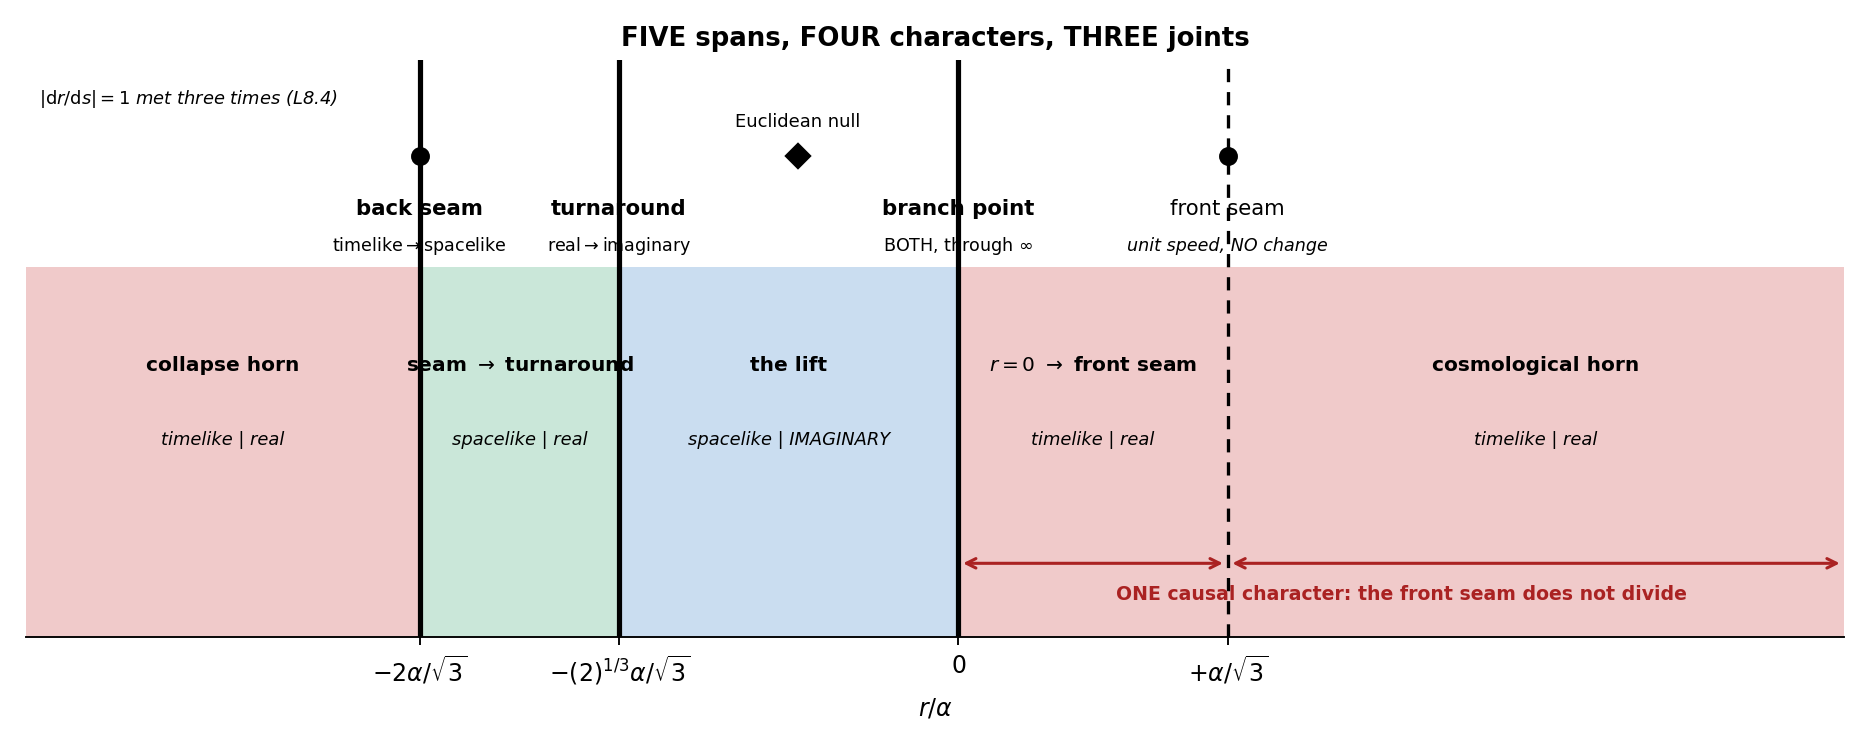
\includegraphics[width=\textwidth]{F_stratification.png}
\caption{\textbf{The causal stratification of the cosmogenetic contour.} Five spans in the signed areal radius,
carrying only \emph{four} distinct causal characters: the sign of $f$ decides whether $r$ is timelike or
spacelike, the sign of $1-f$ whether the marginal congruence's radial rate is real or imaginary. Three joints
carry every change---the back seam (timelike to spacelike), the turnaround (real rate to imaginary), and the
branch point (both at once, through infinity rather than through zero). \emph{The front seam carries none}: on
both sides $r$ is timelike and the rate real, so it is crossed at unit speed without dividing two regions,
which is the geometric face of its being the fixed point of the root-exchange involution~\cite{JanzenGroupoid}.
Marked above: the three passes of the null condition $|\dd r/\dd s|=1$---the two seam passes and the interior
Euclidean null---a \emph{different} triple from the three joints, overlapping them only at the back seam.}
\label{fig:stratification}
\end{figure}

\emph{And the front seam's failure to divide is not an accident of the arithmetic; it is a fixed-point
statement, and the companion groupoid paper has already proved it.} The front seam is the Nariai locus, and
Nariai is the unique fixed point of the root-exchange involution $\sigma$ on the sky-angle circle---the unique
vantage at which the two non-fixed roots of the horizon cubic collide, so that the involution acts trivially
there~\cite{JanzenGroupoid}. A fixed point induces the identity rather than a passage between distinct objects.
That the seam is met at unit speed while changing nothing is the geometric face of that algebraic fact, and it
is the same degeneracy---the double root---that makes the member Nariai, that makes the surface gravity and the
photon orbit's Lyapunov exponent vanish there, and that leaves the degenerate horizon without a bifurcation
sphere. \emph{One degeneracy, read four ways.}

\emph{And these are not three unrelated markings: they are the three solutions of one condition, and together
they are what makes the causal character of the excursion well defined.} In the contour's own path-length
parameter the null condition is $|\dd r/\dd s|=1$, a single equation with no free input, and on the lap it is
met exactly three times---at the seam on the way in, at the interior Euclidean null, and at the seam again on
the way out (Fig.~\ref{fig:F-triptych}, panel \textbf{b}). The turnaround is not among them: there
$\dd r/\dd s=0$, and it \emph{separates} the three. The count is a count of \emph{passes} rather than of
places, since the two seam passes are one substrate point met a lap apart, so the null condition is met three
times at two loci, the Euclidean null being the one met once.

That structure carries the causal reading of the whole excursion, and it is worth saying why the arrangement is
not merely tidy. The lap is the stretch the background represents on a single minimal $S^{3}$ at the throat:
the entire worldline bundle---matter on $r>0$, antimatter on $r<0$, and the photon congruence---is gathered at
the equatorial joint where the two null rulings cross, so one might expect the causal character along it to be
ill defined or to require a choice. It is neither. The character is fixed pointwise by $1-f$, and the three
passes of the null condition are exactly the loci at which it changes: real speed on the lap's real segments,
zero at the turnaround, imaginary on the lift. \emph{And the third pass exists only because the excursion
leaves the real axis.} A contour confined to real cosmic time meets the null condition twice, at the seam's two
passes, and has no way to carry a well-defined causal character across the interval between the turnaround and
the branch point; it is the imaginary excursion---available because the substrate's two real forms are real
forms of one complex group~\cite{JanzenGeometricCore,JanzenBoundary}---that supplies the third pass and closes
the reading. The Euclidean null is therefore not an incidental feature of the lift but the condition on which
the lift's causal well-definedness rests\rcpt{EUCNULL_continuous_null_definition}.

The root triple grades position on the ring---and, read on a fermion sector, the generations~\cite{JanzenMatter}---while these values grade causal character along it. \emph{That the two are one structure is not claimed}: no derivation producing $\{0,1,2\}$ from a single condition with no new input has been exhibited, and the claim is held open\rcpt{LAP_complete_account}.

The lift is the stretch of the contour, of path length $\pi\alpha/3$, along which $\operatorname{Re}\tilde\tau$
does not advance while the areal radius climbs from the comoving turnaround $|r|=(2M\alpha^{2})^{1/3}$ to the
branch point $r=0$. Since $\tilde\tau=is$ there, $\sinh(3is/2\alpha)=i\sin(3s/2\alpha)$, and on the branch
joining the collapse leg the bead's own law reads
\[
r(s)=-(2M\alpha^{2})^{1/3}\bigl\lvert\sin(3s/2\alpha)\bigr\rvert^{2/3},
\]
monotonic from the turnaround to the branch point. With $\dd\tilde\tau=i\,\dd s$ the conformal time
$\dd\eta=\dd\tilde\tau/a$ is \emph{purely imaginary}: the lift is the Euclidean segment of the bead, and the
interior unit-speed locus at $f=2$---the Euclidean null---is the unit-speed condition realised on the imaginary
branch exactly as the seams realise it on the real ones.

\emph{What the segment does is visible in the derivatives.} Along it (Fig.~\ref{fig:F-triptych}, panels
\textbf{b} and \textbf{c}) the rate $\dd r/\dd s$ is carried continuously from \emph{zero} at the turnaround,
through unity at the Euclidean null, to \emph{divergent} at the branch point, with the acceleration growing
without bound over the same interval. And because cosmic time is $\operatorname{Re}\tilde\tau$, which is frozen
there, \emph{the entire process occupies no cosmic time at all}. The lift is not a gap in the cosmic-time
evolution but a single instant of it---a forced phase shift of finite path length and zero duration---which is
why the deparametrized Hamiltonian evolution~\cite{JanzenCanonicalTime} passes from the collapse leg to the
expansion leg with no interval in which to act. A sharp separation follows and is worth recording for the matter
sector: any quantity whose value depends on elapsed cosmic time is necessarily continuous across the lift,
having no time in which to change, while quantities depending on path length or on $\operatorname{Im}\tilde\tau$
may differ across it.

\emph{The universe therefore arrives at $r=0$ carrying exactly the initial data the Friedmann equations require
of it}: vanishing areal radius, divergent expansion rate, and divergent deceleration, the last working against a
rate already large enough to absorb it. This is not a restatement of the standard initial condition but an
account of where it comes from. Eddington pressed the objection against the Einstein--de~Sitter model in 1933,
and pressed it precisely: rival accounts that dispense with a driving force ``necessarily\ldots postulate that
the large velocities have existed from the beginning. This might be true; but can scarcely be called an
\emph{explanation} of the large velocities''; and of the model itself, that it ``leaves me cold. One cannot deny
the \emph{possibility}, but it is difficult to see what mental \emph{satisfaction} such a theory is supposed to
afford''~\cite{Eddington1933}. The objection was never answered; it was retired with its
advocates~\cite{JanzenEinsteinConsiderations}. \emph{The lift answers it.} And in the same passage Eddington set
down, in a footnote, the structure that would supply the requirement---``the system once extended much further
than now, that it collapsed, and is now on the rebound\ldots the inward velocities being turned into outward
velocities by passage through the centre. So far as I know, this is not advocated by anyone''---his stated
reservation being the distribution of velocities, a quantity no one could then compute. What the footnote could
not anticipate is that the passage through the centre is not a point but an interval.

\emph{The explanation is moreover of this framework's characteristic kind, and that is the substance of it rather
than a gloss.} The divergent rate and the divergent deceleration are not dynamical causes acting at a first
instant; they are \emph{effective}---perspectival consequences of continuous parametric motion in $r$ along the
bead, read in a coordinate that is itself a projection. Nothing is driven; the geometry is traversed, and the
dynamics are what that traversal looks like from within. The equations are read leftward from the geometry, and
the beginning ceases to be a mystery requiring new physics at a first moment. That matters independently of this
construction, because the alternative route is closed on general grounds: the decelerative force grows without
bound towards $r=0$, so a quantum-gravitational modification of that point is not a plausible source of an
enormously repulsive first instant~\cite{JanzenEinsteinConsiderations}. \emph{If the initial rate is to be
explained rather than postulated, the explanation must be structural}---and this one is.

\subsection{The quantum reading of the segment}\label{sec:lift-quantum}

The account above is classical, and the same fact that gives it its classical form gives it a quantum one.
Because cosmic time does not advance along the lift, the kernel carrying a state across is not the unitary
$e^{-i\hat{H}\Delta\tau}$ but the Euclidean $K=e^{-\hat{H}\lvert\Delta\eta\rvert}$---consistent with the
evolution operator being the identity, since no cosmic time elapses and the kernel is not an evolution in
cosmic time~\cite{JanzenCanonicalTime}. That kernel damps a mode of frequency $\omega$ by
$e^{-\omega\lvert\Delta\eta\rvert}$, which is the classical selection rule of this section term for term, and
it supplies what the classical reading cannot---it acts on \emph{oscillatory} content only, a frozen,
zero-frequency mode being a fixed point of the kernel. And at the crossing no mode is oscillating---on the contracting leg $aH$ grows without bound as $r\to0$, so the comoving horizon shrinks to zero and every mode exits it and freezes first~\cite{JanzenCRcosmology}---so what the segment removes is the sub-horizon oscillation, that is the acoustic phase, and not the frozen amplitude that crosses. The state it
selects is the one the canonical companion had already fixed on independent grounds---the regular Euclidean
state at the de~Sitter horizon's surface gravity $\kappa=1/\alpha$, used there to close a one-parameter family
of self-adjoint extensions---so the condition closing that quantization and the condition governing the
beginning are one requirement met twice.

The segment is a solution of a variational principle, an instanton in the inverted potential, and in the
gravitational normalisation its Euclidean action is finite and negative,
$S_{E}=-0.0481\,\alpha^{2}/G$: the Hartle--Hawking sign, an enhanced rather than suppressed weight, obtained
from a contour this construction already possessed rather than from a boundary condition imposed to secure it. \emph{The register is worth marking}: the segment's parametrisation runs imaginary, but the continuation is a real analytic one on a spacetime Lorentzian throughout, not a Wick rotation---distinct in kind from the de~Sitter horizon's Gibbons--Hawking continuation, in which $\hbar$ is fixed by the period $\beta=2\pi\alpha$~\cite{JanzenGeometricCore}. \emph{The comparison with the no-boundary sign is therefore a comparison of signs and magnitudes, not an identification of frameworks}, and the action is a real integral along a real curve rather than an exponent awaiting a quantum of action.
The adiabatic correction to the projection is likewise finite---the tower's frequencies diverge at the branch
point but only as $s^{-2/3}$---and larger than the constant-frequency estimate by a factor $2.32$, so the
suppression is stronger than the naive reading gives. \emph{Its adiabaticity is controlled by the harmonic index
alone}, the parameter being $C/\mu_{n}$ with $C\le1.72$, which is of order unity only at $n=2$ and $n=3$.

\section{The central theorem: the augmentation general relativity requires, and the cosmogenesis it forces}\label{sec:central}

The construction to this point has proceeded piece by piece---the horizon's causal structure imported from general relativity, the empirically forced foliation, the layered ontology, the causal reassignment, and the null--boundary correspondence built upon them. We now state, in summation, what those pieces compose: three results, landed together. First, that the CR augmentation is the \emph{necessary and sufficient} completion under which general relativity describes a world that exists and evolves at all---a required augmentation, not an optional interpretation, with its necessary half measured. Second, that on that augmentation gravitational collapse cannot terminate but must continue as a cosmology---collapsed matter becomes a universe, the collapse horizon and the cosmological seam one ontological layer. Third, that this holds for gravitational collapse of \emph{any} symmetry, non-spherical collapse dissolved rather than deferred. The section closes by isolating the one datum these leave open.

We fix the foundational data as established results of the programme's papers (their dependency structure---two streams from the wedge, converging on this framework---is shown in Fig.~\ref{fig:dependency-structure}, and counted in Table~\ref{tab:dependency-matrix}).
\begin{itemize}
\item[(F1)] \emph{The horizon's causal structure}~\cite{JanzenBHcausality}. The event horizon is a metric singularity: no slicing adapted to a finite cosmic time intersects it, every infalling timelike worldline accumulates asymptotically onto its null generators, and it fixes a unique limiting null direction, generically non-orthogonal to any spacelike slice. The horizon is a null hypersurface of topology $S^2\times\mathbb{R}$ foliated by generators that carry a one-way affine ordering. These follow from the Lorentzian causal structure alone and make no use of spherical symmetry.
\item[(F2)] \emph{The singularity taxonomy}~\cite{JanzenCircle,JanzenBHcausality}. The event horizon and the $r=0$ curvature singularity are two species of one genus; the horizon is the finite-curvature species, a substrate-regular null boundary, while the infinite-curvature locus is reached on no finite cosmic layer.
\item[(F3)] \emph{The slicing curve}~\cite{JanzenSlicing}. De~Sitter and Schwarzschild are two readings of one slicing curve on a single de~Sitter substrate, horizons are its turning points, and the Nariai configuration $\Lambda G^2M^2/c^4=1/9$ is the fixed point of the curve's root-exchange involution---the unique tilt whose fundamental worldline meets no horizon.
\item[(F4)] \emph{The reassignment groupoid}~\cite{JanzenGroupoid}. The causal reassignments relating these readings are morphisms of a description groupoid, the discrete symmetry of the solution space, each altering the causal reading of one fixed geometry rather than the geometry.
\item[(F5)] \emph{The forced foliation}~\cite{JanzenModernParallax}. The isotropy of the cosmological redshift measures an objective cosmic rest frame, forcing a cosmic foliation and a uniform expansion from the bottom up; a differential expansion set by the inhomogeneous matter is excluded at the observed level.
\item[(F6)] \emph{The existent}~\cite{JanzenShadowExistence,JanzenCanonicalTime}. Existence is what endures: the evolving spatial layer is the primary existent, and the four-manifold is the representational record of the events that occur as it exists, not an existent of the same kind. The competing readings are closed---``no objective present'' as a modal fallacy, falsified outright by (F5), and ``the block is the existent'' as a category error whose canonical symptom is the frozen problem of time---so that theory-choice, weighing a required structure against a merely permitted one, selects the layered reading.
\end{itemize}

By the \emph{CR augmentation} we mean the single addition these motivate: the primary existent is the evolving spatial layer $\{\mathcal{S}_t\}$, a spacetime $(M,g)$ is its representation under a causal assignment, distinct Lorentzian metrics on one manifold are projections of one layer, and the admissible causal reassignment preserves the cosmic foliation---Einstein's field equations, the Lorentzian metric, and the causal structure left unchanged.

\begin{theorem}[The necessary and sufficient augmentation]\label{thm:augmentation-p7}
Given \textup{(F5)} and \textup{(F6)}, the CR augmentation is necessary and sufficient for a coherent description of a world that exists and evolves---a description of \emph{structural existence}---and it alters no equation of general relativity.
\begin{enumerate}
\item[\textup{(i)}] \emph{Necessary.} A description lacking the ontological lapse collapses existence into occurrence: it grants the four-manifold the existence that belongs to the evolving layer, which on analysis smuggles a fifth, meta-temporal dimension general relativity does not contain and is incoherent as a basic description---the block reading, whose canonical symptom is the frozen problem of time \textup{(F6)}.
\item[\textup{(ii)}] \emph{Sufficient.} Fixing the one physical foliation and reading it ontologically---the lapse the existent's rate of advance, the shift the relativity of synchrony---closes the only coherent escapes: the ``events exist'' horn as that category error, and the ``no objective present'' horn as a modal fallacy, the latter falsified outright by the measured redshift isotropy \textup{(F5)}. No alternative survives.
\end{enumerate}
The necessity is not merely conceptual but \emph{measured}: the physical foliation the lapse requires is not posited but read directly off the redshift isotropy \textup{(F5)}, so that the augmented sub-region of general relativity and the empirically forced foliation are one and the same circle (Fig.~\ref{fig:cr-gr-venn}). The augmentation is thus the structure the world is found to realize, not merely one it may coherently take. This is the theorem of the foundational companion~\cite{JanzenModernParallax}, restated here as the ground of what follows: general relativity becomes a description of structural existence \emph{only} as Cosmological Relativity, and it is forced to.
\end{theorem}

\begin{figure}[ht]
\centering
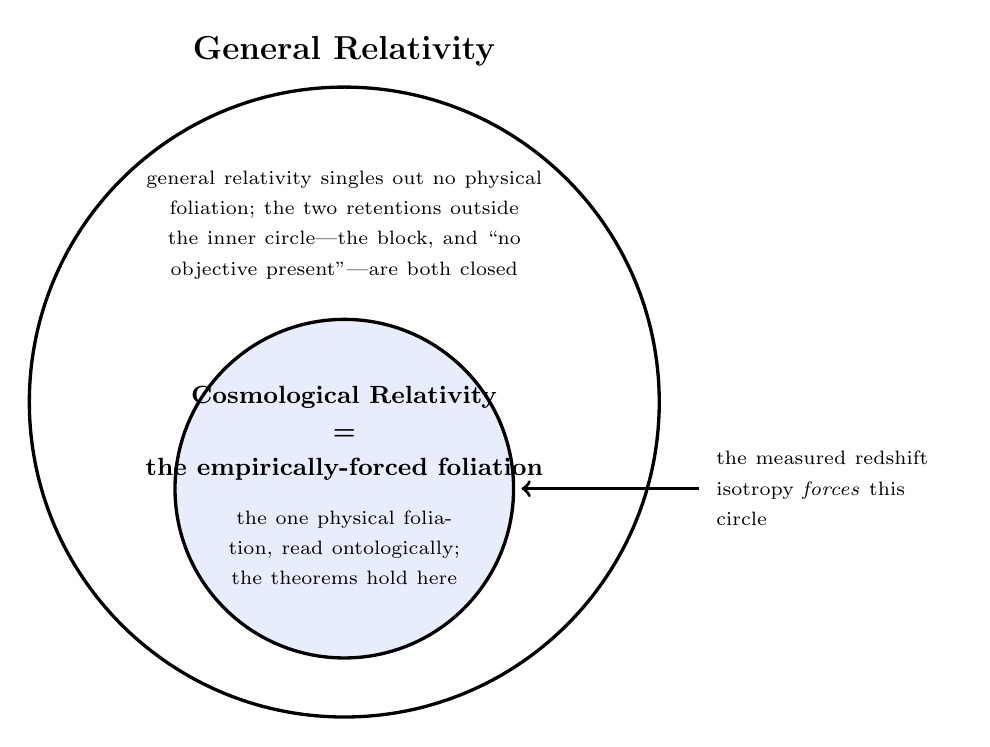
\begin{tikzpicture}[font=\small]
  \draw[very thick] (0,0) circle (4);
  \node at (0,4.45) {\large\textbf{General Relativity}};
  \node[align=center,text width=5.2cm] at (0,2.25)
    {\scriptsize general relativity singles out no physical foliation; the two retentions outside the inner circle---the block, and ``no objective present''---are both closed};
  \draw[very thick,fill=RoyalBlue!12] (0,-1.1) circle (2.15);
  \node[align=center] at (0,-0.4)
    {\textbf{Cosmological Relativity}\\[2pt]$\boldsymbol{=}$\\[2pt]\textbf{the empirically-forced foliation}};
  \node[align=center,text width=3.8cm] at (0,-1.85)
    {\scriptsize the one physical foliation, read ontologically; the theorems hold here};
  \draw[->,very thick] (4.5,-1.1) -- (2.25,-1.1);
  \node[align=left,text width=3cm,anchor=west] at (4.6,-1.1)
    {\scriptsize the measured redshift isotropy \emph{forces} this circle};
\end{tikzpicture}
\caption{Cosmological Relativity as the necessary and sufficient augmentation of general relativity for a description of structural existence (Theorem~\ref{thm:augmentation-p7}). General relativity admits many foliations and singles out none; the augmentation fixes the one physical foliation and reads it ontologically, and by the redshift-isotropy forcing that foliation is measured rather than chosen~\cite{JanzenModernParallax}---so the augmented sub-region of general relativity and the empirically forced foliation are the same circle, and ``CR'' and ``empirically-forced'' are two names for it. The alternatives that would retain general relativity outside the circle are both closed: the block reading as a category error, ``no objective present'' as a modal fallacy falsified by the measured isotropy. Within the circle the programme's theorems hold---the null--boundary correspondence, that collapsed matter must become a universe (Theorem~\ref{thm:cosmogenesis}), for gravitational collapse of any symmetry (Corollary~\ref{cor:nonspherical}).}
\label{fig:cr-gr-venn}
\end{figure}

\begin{figure}[ht]
\centering
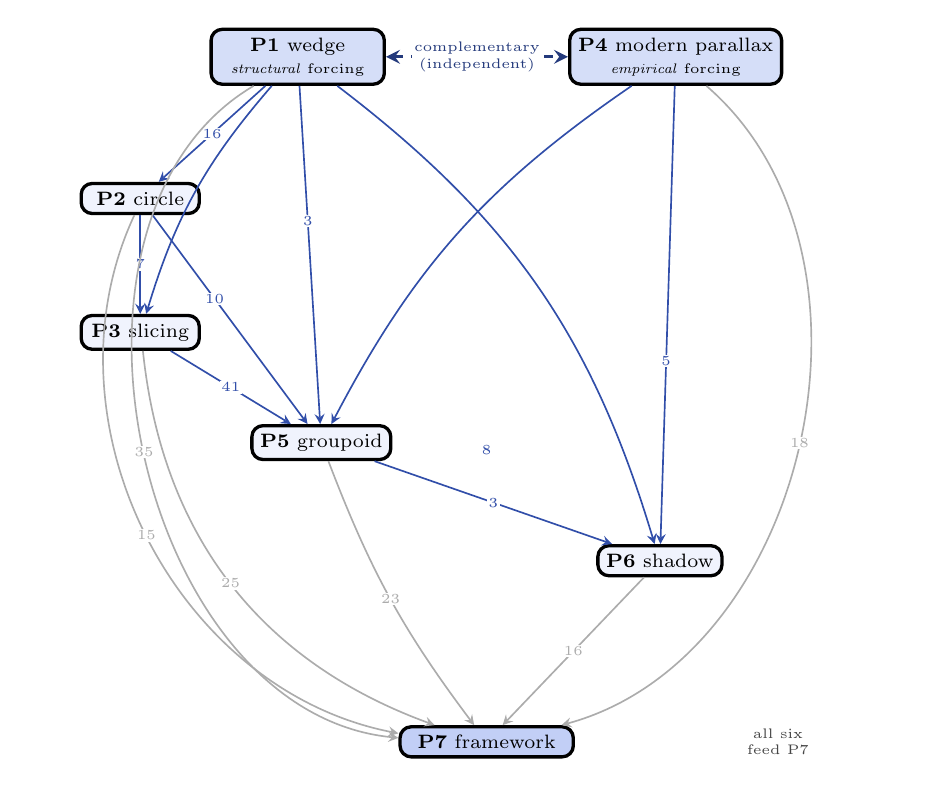
\begin{tikzpicture}[font=\scriptsize,>=stealth,
    pap/.style={draw,very thick,rounded corners,fill=RoyalBlue!8,align=center,inner sep=3pt,minimum width=15mm},
    root/.style={draw,very thick,rounded corners,fill=RoyalBlue!22,align=center,inner sep=3pt,minimum width=22mm},
    conv/.style={draw,very thick,rounded corners,fill=RoyalBlue!32,align=center,inner sep=3pt,minimum width=22mm},
    dep/.style={->,semithick,RoyalBlue!75!black},
    feed/.style={->,semithick,gray!65},
    comp/.style={<->,very thick,dashed,RoyalBlue!55!black},
    wt/.style={midway,fill=white,inner sep=0.6pt,font=\tiny}]

  % two co-equal roots
  \node[root] (P1) at (-2.4,5)  {\textbf{P1} wedge\\\tiny \emph{structural} forcing};
  \node[root] (P4) at (2.4,5)   {\textbf{P4} modern parallax\\\tiny \emph{empirical} forcing};
  \draw[comp] (P1) -- (P4) node[midway,align=center,fill=white,inner sep=1pt,font=\tiny,text=RoyalBlue!55!black]{complementary\\(independent)};

  \node[pap] (P2) at (-4.4,3.2) {\textbf{P2} circle};
  \node[pap] (P3) at (-4.4,1.5) {\textbf{P3} slicing};
  \node[pap] (P5) at (-2.1,0.1) {\textbf{P5} groupoid};
  \node[pap] (P6) at (2.2,-1.4) {\textbf{P6} shadow};
  \node[conv](P7) at (0,-3.7)   {\textbf{P7} framework};

  % --- inter-paper dependency edges (all of them) ---
  \draw[dep] (P1) -- (P2) node[wt]{16};
  \draw[dep] (P1) to[bend right=12] (P3) node[wt,pos=0.6]{3};
  \draw[dep] (P1) -- (P5) node[wt,pos=0.4]{3};
  \draw[dep] (P1) to[bend left=18] (P6) node[wt,pos=0.7]{5};
  \draw[dep] (P2) -- (P3) node[wt]{7};
  \draw[dep] (P2) -- (P5) node[wt,pos=0.4]{10};
  \draw[dep] (P3) -- (P5) node[wt]{41};
  \draw[dep] (P4) to[bend right=14] (P5) node[wt,pos=0.12]{8};
  \draw[dep] (P4) -- (P6) node[wt,pos=0.6]{5};
  \draw[dep] (P5) -- (P6) node[wt]{3};

  % --- all six feed the framework P7 (the compounding) ---
  \draw[feed] (P1) to[bend right=72] node[wt]{35} (P7);
  \draw[feed] (P2) to[bend right=52] node[wt]{15} (P7);
  \draw[feed] (P3) to[bend right=32] node[wt]{25} (P7);
  \draw[feed] (P5) to[bend right=8]  node[wt]{23} (P7);
  \draw[feed] (P6) -- node[wt]{16} (P7);
  \draw[feed] (P4) to[bend left=62]  node[wt]{18} (P7);
  \node[font=\tiny,text=gray!55!black,align=center] at (3.7,-3.7) {all six\\feed P7};
\end{tikzpicture}
\caption{The foundational structure the central theorem rests on (edge labels are citation multiplicities, a proxy for load-bearing weight---and a proxy this figure cannot itself test, its six feeds being too few: the correlation between a paper's feed count and its length is $r=+0.18$ with a $95\%$ interval running from $-0.74$ to $+0.87$, which excludes nothing\ldg{statistics_inference}). The construction stands on \emph{two co-equal foundational forcings, neither depending on the other}: the wedge P1---a \emph{structural} forcing (the event horizon as a metric singularity, local causal structure, proven from general relativity alone)---and modern parallax P4---an \emph{empirical} forcing (the redshift-isotropy floor, precision cosmology and its structural consequences). Their cross-references are \emph{complementary, not dependent}: each cites the other precisely to record that its own result ``stands on causal structure alone and needs none of'' the other's evidence~\cite{JanzenBHcausality,JanzenModernParallax}, P4 the empirical counterpart of P1's conceptual result. From the structural root the geometry chain descends (P1$\to$P2$\to$P3$\to$P5), but the structure is a \emph{dense weave, not a chain}: most papers feed several downstream directly (P2, for instance, into P3, P5, \emph{and} P7), and \emph{all six} feed the framework P7 (F1--F6 of Theorem~\ref{thm:augmentation-p7})---the compounding that makes the corpus a convergence rather than a line. Every dependency edge is drawn; blue arrows are inter-paper dependencies, grey the six feeds into P7, the dashed link the P1--P4 complementarity. P7 leans heaviest on the structural forcing (${\times}35$, reaching P7 both through the chain and directly via the horizon's null structure the null--boundary correspondence uses), with the empirical forcing at ${\times}18$. The framework is the convergence of two independent forcings, structural and empirical, of one cosmic foliation. [Full direct feed into P7: P1~${\times}35$, P3~${\times}25$, P5~${\times}23$, P4~${\times}18$, P6~${\times}19$, P2~${\times}15$.]}
\label{fig:dependency-structure}
\end{figure}

\begin{table}[ht]
\centering
\scriptsize
\setlength{\tabcolsep}{4pt}
\renewcommand{\arraystretch}{1.25}
\resizebox{\textwidth}{!}{%
\begin{tabular}{r|ccccccccccccccccc}
 & \multicolumn{17}{c}{\footnotesize\emph{$\cdots$ draws on (cited paper) $\to$}}\\[1pt]
\footnotesize\emph{paper} & P1 & P2 & P3 & P4 & P5 & P6 & P7 & P8 & P9 & P10 & P11 & P12 & P13 & P14 & P15 & P16 & p0\\
\hline
P1 \; wedge & -- & 5 & 2 & $\lozenge$2 & . & 2 & 11 & . & . & 2 & 2 & . & . & . & 5 & 2 & 2\\
P2 \; circle & 16 & -- & 28 & 2 & 2 & 4 & 11 & 5 & 4 & . & . & 1 & 3 & 4 & 1 & 3 & 6\\
P3 \; slicing & 3 & 7 & -- & . & 15 & 2 & 20 & 3 & 4 & . & . & 4 & 11 & 24 & 2 & 3 & 16\\
P4 \; mod.\ parallax & $\lozenge$4 & . & . & -- & . & 5 & 8 & 3 & 3 & 1 & . & . & . & . & . & 2 & 1\\
P5 \; groupoid & 3 & 10 & 41 & 8 & -- & 3 & 20 & . & 5 & . & 1 & 6 & 7 & 5 & . & 3 & 5\\
P6 \; shadow & 5 & 4 & 6 & 5 & 3 & -- & 11 & 1 & 1 & 3 & . & 2 & 1 & 4 & 3 & 3 & 4\\
\textbf{P7 \; framework} & \textbf{35} & \textbf{15} & \textbf{25} & \textbf{18} & \textbf{23} & \textbf{16} & -- & \textbf{15} & \textbf{11} & \textbf{20} & \textbf{13} & \textbf{13} & \textbf{21} & \textbf{29} & \textbf{31} & \textbf{12} & \textbf{14}\\
P8 \; operator & 2 & 7 & 8 & 2 & 2 & 4 & 16 & -- & 6 & 3 & 2 & 2 & . & 2 & 3 & 4 & 4\\
P9 \; range & . & 2 & 3 & . & 2 & 1 & 11 & 9 & -- & . & 6 & 3 & 3 & 1 & 2 & 3 & 3\\
P10 \; canon.\ time & 7 & 1 & 3 & 4 & 1 & 3 & 19 & 4 & 2 & -- & 2 & 2 & 1 & . & 2 & 2 & 8\\
P11 \; dynamics & 3 & 1 & 5 & 1 & 3 & 1 & 11 & 4 & 12 & 6 & -- & 4 & 4 & 3 & 2 & 2 & 3\\
P12 \; algebroid & 3 & . & 10 & 3 & 7 & 2 & 4 & 6 & 12 & 5 & 4 & -- & 2 & 4 & . & 2 & 7\\
P13 \; boundary & 1 & 1 & 8 & 1 & 5 & 2 & 13 & 5 & 6 & 6 & 3 & 15 & -- & 30 & 3 & 3 & 9\\
P14 \; matter & . & 3 & 16 & . & 4 & 3 & 10 & 3 & 1 & 2 & 3 & 9 & 23 & -- & 1 & 2 & 9\\
P15 \; cosmology & 4 & 3 & 8 & 8 & 3 & 4 & 19 & 12 & 4 & 4 & 3 & 1 & . & 3 & -- & 17 & 4\\
P16 \; cosmogenesis & 2 & 4 & 3 & 1 & 1 & 3 & 12 & 7 & 4 & 3 & 1 & 1 & 4 & 3 & 12 & -- & 2\\
\textbf{p0 \; core} & \textbf{2} & \textbf{2} & \textbf{25} & \textbf{7} & \textbf{10} & \textbf{4} & \textbf{17} & \textbf{6} & \textbf{5} & \textbf{6} & \textbf{5} & \textbf{13} & \textbf{20} & \textbf{14} & \textbf{10} & \textbf{3} & --\\
\end{tabular}%
}
\caption{The corpus's complete internal dependency matrix over all sixteen papers and the geometric core p0 (P1 wedge, P2 circle, P3 slicing, P4 modern parallax, P5 groupoid, P6 shadow, P7 framework, P8 operator, P9 range, P10 canonical time, P11 dynamics, P12 algebroid, P13 boundary, P14 matter, P15 cosmology, P16 cosmogenesis, p0 geometric core), extracted from citation counts (a proxy for load-bearing weight): entry $(i,j)$ is the number of times paper $i$ cites paper $j$; ``\,.\,'' is none, ``--'' the diagonal. \emph{Read a row} for what a paper rests on; \emph{read a column} for what it feeds. The two \emph{roots} P1 and P4 carry near-empty dependency rows, and the $\lozenge$ entries mark their relation as \emph{complementarity, not dependency} (\S\ref{sec:central}). The framework \textbf{P7} (bold) is the convergence---the single heaviest row, drawing directly on \emph{every} other document---and P3 (slicing) the most-drawn-on hub. \textbf{P16} (cosmogenesis) enters as the synthesis it names: its row draws on the whole spine it conjoins---leaning hardest on the cosmology P15 and the operator P8 (the leaf-carried density its rate-handoff rests on)---and its column shows the whole corpus now points into it, every paper P1--P15 citing it, the forward-pointers of the reciprocity pass. The geometric core p0 is the second synthesis pole: every paper feeds it and it points back into the corpus; and its own row is now current---it cites every paper, including its return of P16, the wrapper's collection of the whole corpus complete. The whole is a dense weave, not a line.}
\label{tab:dependency-matrix}
% MAINTENANCE: the matrix is 17x17 with alias-resolved counts recomputed from source by
% scripts/depmatrix.py (canonical resolver in BIBKEY_ALIAS_MAP.md). Re-run it after any
% citation change, and harmonise fig:dependency-structure's feeds and edges to match.
\end{table}

\begin{table}[ht]
\centering
\scriptsize
\setlength{\tabcolsep}{4pt}
\renewcommand{\arraystretch}{1.15}
\resizebox{\textwidth}{!}{%
\begin{tabular}{r|ccccccccccccccccc}
 & \multicolumn{17}{c}{\footnotesize\emph{$\cdots$ is drawn on by (paper) $\to$}}\\[1pt]
\footnotesize\emph{ledger} & P1 & P2 & P3 & P4 & P5 & P6 & P7 & P8 & P9 & P10 & P11 & P12 & P13 & P14 & P15 & P16 & p0\\
\hline
\textsf{algebraic geometry} & . & . & 1 & . & 1 & . & . & . & 1 & . & . & . & . & . & . & . & .\\
\textsf{cartan holonomy} & . & . & . & . & . & . & . & . & . & . & 1 & 1 & . & 2 & . & . & .\\
\textsf{catastrophe singularity} & . & 1 & . & . & . & . & 1 & 1 & . & . & . & . & . & . & . & . & .\\
\textsf{category theory} & . & . & . & . & 1 & . & . & . & . & . & . & 1 & . & . & . & . & 1\\
\textsf{combinatorics} & . & . & 1 & . & . & . & 2 & . & . & . & . & . & . & 1 & . & . & 1\\
\textsf{complex analysis} & . & 1 & . & . & 2 & . & . & . & . & . & . & 1 & . & . & . & 1 & .\\
\textsf{conformal geometry} & . & . & 2 & . & . & . & . & . & . & . & . & . & . & 1 & . & . & 1\\
\textsf{convexity optimisation} & . & . & . & . & . & . & . & . & . & . & . & . & . & . & . & . & .\\
\textsf{functional analysis} & 2 & . & . & . & . & . & . & . & 1 & 1 & 1 & . & . & 1 & . & . & 1\\
\textsf{harmonic analysis} & . & . & 1 & 1 & . & . & . & . & . & . & . & . & . & . & . & . & 1\\
\textsf{involution real forms} & . & . & . & . & . & . & . & . & . & . & . & . & 2 & . & . & . & .\\
\textsf{optics lensing} & . & . & . & . & . & . & 2 & . & . & . & . & . & . & . & 1 & . & .\\
\textsf{quadric geometry} & . & . & 1 & . & 1 & . & . & . & . & 1 & . & . & . & . & . & . & 2\\
\textsf{representation theory} & . & . & 2 & . & . & . & . & . & . & . & . & . & . & 1 & . & . & .\\
\textsf{spectral theory} & . & . & 1 & . & 1 & . & . & . & 1 & . & . & . & . & 2 & 1 & . & 1\\
\textsf{statistics inference} & . & . & . & 1 & . & . & 1 & . & . & . & . & . & . & . & . & 1 & .\\
\textsf{variational} & . & . & . & . & 1 & . & . & 1 & 1 & 1 & . & . & . & . & . & . & .\\
\textsf{figure theorem} & . & 1 & 2 & . & 1 & . & 1 & . & . & . & . & . & . & . & . & . & 6\\
\textsf{information theory} & . & . & . & . & . & . & . & . & . & . & . & . & . & . & 1 & 1 & 1\\
\textsf{number theory} & . & . & . & . & 1 & . & . & . & . & . & . & . & . & . & . & . & 1\\
\textsf{numerical analysis} & . & . & . & . & 1 & . & . & . & . & . & . & . & . & . & 2 & . & .\\
\textsf{probability} & . & . & . & 2 & . & . & . & . & . & . & . & . & . & . & . & . & .\\
\textsf{index theory} & 1 & . & . & . & . & 1 & . & 1 & . & . & . & 1 & . & 2 & . & . & 1\\
\textsf{integrable systems} & 1 & 1 & 1 & 1 & 1 & 1 & . & 1 & 1 & 1 & . & 1 & 1 & 1 & 1 & 1 & 1\\
\end{tabular}}
\caption{\emph{The worked mathematics the corpus draws on.} Rows are the programme's knowledge ledgers---seventeen field bakes and the figure--theorem bake---and entries count \ldgmarker\ markers, one per claim in that paper resting on that bake. Read beside Table~\ref{tab:dependency-matrix}, a column gives a paper's own sources and then the mathematics under them. \emph{A zero is a finding rather than a gap}: a field that legitimately gave a paper nothing must be legible as such, and each ledger's landing table carries the reason.}
\label{tab:ledger-block}
% MAINTENANCE: rows recomputed from source by scripts/depmatrix.py, which reads the ledger set from
% corpus/ledgers_registry.md at run time -- never hard-code the row count, more fields are queued.
\end{table}


\begin{theorem}[Collapsed matter must become a universe]\label{thm:cosmogenesis}
On the augmentation of Theorem~\ref{thm:augmentation-p7}, gravitational collapse cannot terminate; it continues as a cosmology. The limiting null direction of any collapse horizon \textup{(F1)}, reassigned on the forced foliation \textup{(F5)} by a foliation-preserving morphism \textup{(F3, F4)}, is the fundamental timelike congruence of a Schwarzschild--de~Sitter representation of the same ontological layer; its cosmological member is fixed to the Nariai configuration \textup{(F3)}, its evolution is the $\sinh^{2/3}$ law of flat $\Lambda$CDM, and the collapse horizon $\mathcal{H}^+$ and the de~Sitter cosmological horizon $\mathcal{H}_c^{+}(p)$ are one ontological layer under distinct causal assignments \textup{(Theorem~\ref{thm:null-boundary})}, the $S^3$ family of reassigned horizons being that congruence. The completion of collapse is therefore not an interior curvature singularity---which no finite cosmic layer ever reaches \textup{(F1, F2)}---but the finite-curvature cosmological seam: the future of the collapsed matter \emph{is} an expanding universe.
\end{theorem}

\begin{proof}
By Theorem~\ref{thm:augmentation-p7} the layered ontology and its forced foliation are in force. (F1) supplies the limiting null direction and the horizon's $S^2\times\mathbb{R}$ generator structure; the reassignment of \S\ref{sec:reassignment}, a foliation-preserving morphism of the groupoid (F4) on the forced foliation (F5), promotes that null congruence to the timelike fundamental congruence; the alignment selection (\S\ref{sec:sds-cosmology}, from F1 and F3) fixes the Nariai member; and Theorem~\ref{thm:null-boundary} establishes $\mathcal{N}:\mathcal{H}^+\to\mathcal{H}_c^{+}(p)$ with the bijection $p\mapsto\mathcal{H}_c^{+}(p)$ under which the $S^3$ of reassigned horizons is the comoving congruence carrying the $\sinh^{2/3}$ evolution [Eq.~\eqref{eq:r-SdS-solution}]. That the interior curvature singularity is reached on no finite cosmic layer is (F1)--(F2). The future of the collapse is therefore the cosmological seam, and the continuation of its matter is the expansion.
\end{proof}

\begin{remark}[The matter of the collapse]
The ``collapsed matter'' whose future is our expansion sits, by Theorem~\ref{thm:bead}, on the conjugate ($r<0$) branch of the one bead---the antimatter branch, the $R=\gamma^5$ reflection of our expansion leg. Read at the level of that signed-radius geometry the progenitor is therefore an antimatter black hole relative to the cosmos it seeds, our matter and its being the two ends of one conjugation across the $r=0$ branch point (Theorem~\ref{thm:antimatter-progenitor}); by CPT this is the same statement its own observers would make of us. The claim is carried by the branch geometry alone, and does not rest on the branch-point crossing dynamics of a concrete matter model, which \S\ref{sec:frontiers} settles separately.
\end{remark}

\begin{corollary}[Dissolution of non-spherical collapse]\label{cor:nonspherical}
The correspondence of Theorem~\ref{thm:cosmogenesis} holds for gravitational collapse of any symmetry that forms a horizon; non-spherical collapse is not a distinct case.
\end{corollary}

\begin{proof}
The correspondence $\mathcal{N}$ is causal and structural, not metric (Theorem~\ref{thm:null-boundary}): it maps the generator fibration, the affine ordering, and the future orientation, and carries no horizon area, surface gravity, or metric multipole. Its sole datum on the collapse side is the horizon's causal structure (F1)---a null hypersurface $S^2\times\mathbb{R}$ foliated by generators of one-way ordering onto which infalling worldlines accumulate---which is the general structure of any four-dimensional event horizon and holds independently of spherical symmetry. An aspherical progenitor radiates its higher multipoles as it settles, so its horizon carries only the diffeomorphism-invariant data $(M,J,Q)$ encoded on the null boundary (the no-hair structure, \S\ref{sec:null-boundary-correspondence}); the aspherical detail is absent from the boundary the correspondence reads. A non-spherical collapse therefore presents the same causally-typed null boundary as a spherical one and is carried to the same de~Sitter cosmological seam by the same $\mathcal{N}$. Of the invariants that do survive on the boundary, the symmetry-reducible ones---rotation and NUT charge---are already cuts of the substrate, members of the reachable Kerr--NUT--(A)dS kernel classified in the range~\cite{JanzenRange}, while genuinely inhomogeneous collapse lies past the wall of inhomogeneity, where the construction's generation-by-symmetry hands off to ordinary Einstein evolution~\cite{JanzenRange,JanzenDynamics}. In neither register is ``non-spherical collapse'' a separate correspondence to be built.
\end{proof}

\begin{remark}[The one open frontier]
The single datum Theorem~\ref{thm:cosmogenesis} does not fix is the \emph{irreducible} interior remainder---the Kerr-inner and Reissner--Nordstr\"om-interior reassignments---which lie across the matter side, in the interior geometry the exterior correspondence does not read. Corollary~\ref{cor:nonspherical} sharpens what that leaves: the exterior correspondence being symmetry-independent, what remains is not a wider class of collapses but the interior remainder alone. \emph{The crossing itself is not among it}---the matter branch-point crossing is settled on the field side and on the worldline side, and the two halves answer each other, as the frontiers section sets out; what stays open there is the interior reassignment, which is ordinary interior analysis rather than a frontier of this construction.
\end{remark}

\begin{remark}[Scope]
The two theorems are a necessity and sufficiency \emph{internal to the framework's foundations}: given (F1)--(F6), the CR augmentation is the required completion for a description of structural existence (Theorem~\ref{thm:augmentation-p7}), and on it collapse must continue as a cosmology (Theorem~\ref{thm:cosmogenesis}), with (F5) the empirical anchor of the necessary half. What is \emph{not} claimed is that the observed cosmos matches that cosmology in every measured detail; that soundness is held to the two tests the programme keeps open---the structural test of the metric-singularity result, that closed trapped surfaces do not form and collapse does not complete in finite cosmic time~\cite{JanzenBHcausality}, and the empirical test of the cosmology~\cite{JanzenCRcosmology}.
\end{remark}

\section{Synthesis and Structural Closure of the Programme}\label{sec:synthesis}

\subsection{Two crossable boundaries, of opposite type}\label{sec:two-boundaries}

One structural observation belongs at the head of the synthesis, because it is what several of the results
below have in common and it is not visible from any of them alone. The construction crosses two boundaries at
which the standard reading would stop, and \emph{it crosses them for opposite reasons}.

At the event horizon the curvature is finite while the tortoise measure diverges: $f\to0$, so
$r_{*}=\int\dd r/f$ grows without bound as the boundary is approached, and the crossing is licensed by the
geometry being regular there---the horizon is a \emph{metric} singularity, at which the spatial measure
collapses while the curvature does not~\cite{JanzenBHcausality}. At the branch point of the cosmogenetic
contour the reverse holds. There $f\to-2M/r$ diverges, so \emph{$r_{*}$ converges}---the crossing carries no
scale---while the areal curvature diverges without limit, and $r=0$ remains a genuine infinite-curvature
locus~\cite{JanzenCircle}. Each boundary is crossable; neither is crossable for the other's reason.

\emph{What this says about the standard verdict is the substance of it.} ``Singularity'' is habitually read as
a single condition, with curvature blow-up and geodesic incompleteness treated as two faces of one fact. They
are independent, and this construction realises each without the other: a boundary with finite curvature and
divergent measure, and a boundary with divergent curvature and finite measure. The singularity theorems'
criterion is the second of these---incompleteness in an affine measure---and it is the one the horizon fails to
meet while the branch point meets it in a form that continues rather than terminates. \emph{A boundary is
passable if either failure is absent, and the two failures do not coincide anywhere in this construction.}

That is also what makes the imaginary-time segment of the contour a well-posed object rather than a formal
manoeuvre. The segment terminates at the branch point, where the curvature diverges; but it is crossed over a
\emph{finite} imaginary interval with $r_{*}$ finite, so the divergence obstructs
nothing~\cite{JanzenCanonicalTime}. The same complementarity that lets the collapse be read as a cosmology lets
the beginning be read as a continuation.

The central theorem (\S\ref{sec:central}) established the collapse--cosmology closure formally: the augmentation general relativity requires for a description of structural existence is the one under which the horizon-selected null direction becomes the cosmic congruence, so that collapse continues as the Nariai Schwarzschild--de~Sitter cosmology and the expansion history of the real universe is set by the single scale $\Lambda$. Three consequences of that closure are worth recording before the reach is widened. First, because no finite ontological layer contains a point-mass configuration, density remains finite on every finite cosmic slice. Second, because the SdS expansion is observationally indistinguishable from flat $\Lambda$CDM at late times but differs at early times, the framework offers empirical avenues for distinguishing representational cosmologies while retaining full agreement with the tested predictions of general relativity---the discriminators the companion cosmology paper carries to the microwave background~\cite{JanzenCRcosmology}. Third, the single scale reaches down as well as out: the same $\Lambda$ that sets the expansion sets, for every mass, the local boundary at which a structure's gravitational hold gives way to the cosmic flow---the Hubble--Eddington radius~\cite{Eddington1933} $r_{\mathrm{HE}}=(M\alpha^{2})^{1/3}$, which the slicing geometry reads as the flat locus of the existent slice, the local bend of the cut cancelling the substrate's cosmological curvature~\cite{JanzenSlicing,JanzenOperator}. The long-standing local--cosmic boundary---whether and where structure partakes in the expansion---is thereby a per-structure geometric locus, one substrate $\Lambda$ read at two ranges.

\subsection{The general reach: the symmetry-reducible sector as one substrate's cuts}\label{sec:general-reach}

The closure above is drawn for the collapse--cosmology pair, but the same construction, developed in the companion papers, reaches the whole symmetry-reducible vacuum sector of general relativity, and it is worth setting out both what that reach amounts to and---as sharply---what it does not. The slicing operator promotes the de~Sitter slicing curve from a classifier of the SdS family to a generator of the static, spherically symmetric sector, with the vacuum solutions the kernel of the matter functional and matter the bend of the cut off that kernel~\cite{JanzenOperator}; the range of that operator is exactly the symmetry-reducible sector---a geometry is a cut of the substrate precisely when its isometry group contains a sweep-subgroup of the substrate's---filled across every Petrov type, the vacuum members the substrate's own families (from Schwarzschild--de~Sitter through the rotating Kerr--NUT--(A)dS family to the functional Weyl class) and matter the bend throughout, bounded by a wall at which continuous symmetry, and with it the generative reach, is lost~\cite{JanzenRange}. What general relativity holds as a catalogue of separate exact solutions is, in this reading, the family of cuts of one de~Sitter substrate whose only scale is the throat radius $\alpha=\sqrt{3/\Lambda}$: general relativity's own covariance---one geometry under change of chart---lifted one level, to one substrate under change of geometry, with the slicing curve the gauge object.

This reach answers, for the reducible sector, the classification question this programme places on the table (\S\ref{sec:frontiers}): how much of the standard catalogue of exact solutions is geometric multiplicity and how much is vantage. The apparent multiplicity of the reachable catalogue decomposes on three orthogonal axes. \emph{Vantage} multiplicity is a finite groupoid of causal readings of \emph{one} fixed cut---the backward-radial reflection $r\mapsto-r$ exchanging de~Sitter and Schwarzschild~\cite{JanzenSlicing,JanzenGroupoid}, the orientation parity $\pm M$ exchanging the black-hole and naked readings~\cite{JanzenAlgebroid}, the slicing reassignment relating the Kantowski--Sachs and flat-FLRW readings of one Schwarzschild--de~Sitter geometry (differing by the rest-energy term alone)~\cite{JanzenRange}, and the null$\leftrightarrow$timelike reassignment relating the collapse interior to the expanding cosmology~\cite{JanzenCRcosmology}---each changing the reading, not the geometry, and organised as the discrete symmetry of the solution space~\cite{JanzenGroupoid}. \emph{Geometric} multiplicity is the moduli of genuinely distinct vacuum cuts within the reachable classes: the vacuum kernels of the range---the one-parameter Schwarzschild--de~Sitter family, the separable Type-D family Kerr--NUT--(A)dS, the functional Weyl class, the homogeneous Bianchi families---with mass, rotation, and NUT charge the moduli transverse to the substrate's orbits~\cite{JanzenRange,JanzenAlgebroid}. And \emph{matter} enters on a third axis orthogonal to both: charge and acceleration are not vacuum cuts but bends off the kernel~\cite{JanzenRange}. The reducible catalogue is therefore \emph{one substrate read through a finite vantage groupoid, over a moduli family of vacuum cuts, with matter the bend}; algebraic type is no constraint on the reach (types O, D, I all filled), and Type~D is the separable corner where the substrate's symmetry surfaces as the Carter constant rather than the edge. The Friedmann initial singularity, on this classification, is the cosmogenesis branch point \emph{of} the degenerate Nariai member of the homogeneous kernel~\cite{JanzenRange}---a boundary of the cut, not a breakdown of the geometry, its curvature divergent but its tortoise measure finite, which is why the crossing carries no scale. \emph{The branch point and the Nariai member are not the same locus}: the branch point is at $r=0$ and the Nariai member is seeded at $\alpha/\sqrt3$, and this paper elsewhere lists those as quantities never to be conflated. What the reducible classification leaves open is the \emph{irreducible} interior remainder: the Kerr-inner and Reissner--Nordstr\"om-interior reassignments, which tie to the matter side and lie in the interior geometry the reducible classification does not reach.

These vantage readings are of one ontological layer, not autonomous geometries on distinct realities. By the ontological event individuation of \S\ref{sec:CR-hole} and the metric reassignment of \S\ref{sec:reassignment}, de~Sitter, Schwarzschild, and the Nariai cosmology are distinct Lorentzian geometries representing a single layer---the de~Sitter manifold and its invariant $\alpha$ themselves invariants of the representation, the individuating entity the layer, realised as readings of one slicing curve~\cite{JanzenSlicing}. Of the discrete relations among those readings, the within-geometry vantage-change is a Weyl reflection of the horizon triple fixed at the Nariai cosmology, while the de~Sitter$\leftrightarrow$Schwarzschild correspondence is the $A_2$ diagram automorphism, the backward-radial reflection under which the de~Sitter geometry is fixed and the Schwarzschild mass reversed; the two together generate the full discrete symmetry $\mathrm{Aut}(A_2)=D_6$~\cite{JanzenGroupoid,JanzenAlgebroid}. That symmetry is itself orthogonal in the sense this section's decomposition uses: $D_6=S_3\times\mathbb{Z}_2$ is a \emph{direct} product, its factors acting on independent structures---the Weyl $S_3$ on the three horizon roots, the reflection on the substrate's two null rulings---so the vantage axis carries two sub-axes rather than one graded list, and the independence is geometric: the roots are the three points \emph{on} the throat circle and the rulings the lines \emph{tangent} to it, and \emph{on} and \emph{tangent} are independent relations to one circle~\cite{JanzenGeometricCore,JanzenMatter}.

\subsection{The two-sided closure: matter and antimatter, and charge conjugation as the cosmogenesis's face}\label{sec:two-sided-closure}

The reflection factor just isolated---$R$ on the substrate's two null rulings, the $\mathbb{Z}_2$ of $\mathrm{Aut}(A_2)=D_6$---is the hinge of a closure the programme carries in full, and it is set down here as the result it is rather than deferred as a frontier. $R$ is the mass-reflection $r\mapsto-r$ ($2M\mapsto-2M$), a linear isometry whose sole fixed point is the bead's own $r=0$ crossing and which exchanges the two species-regions $r>0$ and $r<0$ bijectively; under $R=\gamma^5$ the collapse leg ($r<0$) is the antifundamental $\bar{\mathbf 3}=R(\mathbf 3)$ of the matter branch, so within CR it is antimatter at the weight the fundamental branch is matter, and the completed collapse whose future is our expansion is, in the signed-radius continuation, an antimatter black hole (Theorem~\ref{thm:antimatter-progenitor}). That is the real, linear face. The substrate carries a second, antilinear face of the same object: the reality involution $K:\tilde\tau\mapsto\bar{\tilde\tau}$ on complexified cosmic time---complex-analytic and geometric---which fixes the neutral real axis, the self-conjugate photon congruence, and swaps the two conjugate wings of the lap. $R$ and $K$ are the two axis-symmetries of one analytic object, the plate $\mathbb{C}_r\times\mathbb{C}_{\tilde\tau}$: the $r$-axis carrying $R$ with the $A_2$ hexad and the two rulings, the $\tilde\tau$-axis carrying $K$ with the cosmogenetic lap and its two wings. The substrate's two rulings and the lap's two wings are therefore \emph{not} two candidates awaiting a single assignment but the linear and antilinear faces of that one plate---the rulings borne on $R$'s $r$-axis, the wings on $K$'s $\tilde\tau$-axis---meeting at the $r=0$ crossing that is $R$'s fixed point and the branch point the cosmogenesis completes~\cite{JanzenBoundary}.

Their composite closes charge conjugation. $R\circ K$ is an antilinear involution reproducing $C$'s action on species, on $|2M|$, on the mass-sign, and on the Feynman--St\"uckelberg particle$\leftrightarrow$antiparticle wing structure, while being blind to the electric-charge sign---the metric carrying charge only through $Q^{2}$---so charge conjugation factorises, $C=(Q\mapsto-Q)_{\mathrm{field}}\circ(R\circ K)_{\mathrm{geometric}}$, the substrate supplying every kinematic ($CPT$/Feynman--St\"uckelberg) datum of $C$ and only the electric-charge sign closing from the matter field~\cite{JanzenBoundary}. The geometric factor's fixed point \emph{is} the bead's $r=0$ crossing, so the vertex on which charge conjugation's kinematic face turns is the very seam that completes collapse into our expansion: charge conjugation and the cosmology are one structure, read off the one plate, the discrete residue of matter and the conjugation of charge two faces of a single object. The built fermion sector realises that face on its actual zero-modes, $R$ carrying each generation's wall-mode to its bound opposite-chirality antimatter partner~\cite{JanzenMatter}. What the two-sided structure leaves genuinely open is narrow, and is the matter sector's rather than the framework's: the identification of a wing with a \emph{specific} charged particle, the full antilinear $C$ whose charge sign closes from the field, and the world-correspondence of the reading---each carried and weighed in the companion boundary and matter papers~\cite{JanzenBoundary,JanzenMatter}. The two-sided structure itself---rulings and wings, matter and antimatter, charge conjugation and cosmogenesis as the $R$ and $K$ faces of one plate---stands closed.

\subsection{Standing features of general relativity, recovered}

Three standing features of general relativity are recovered as consequences of that single structure rather than as separate inputs. The hidden symmetry of the Type-D family---the Killing tensor and Carter constant that render Kerr geodesics integrable, which general relativity carries without explanation---is the substrate's own maximal symmetry surfacing in the separable corner~\cite{JanzenRange}. The canonical problem of time---the frozen Hamiltonian constraint of the Dirac algebra---is not a defect awaiting a technical repair but the canonical face of reading the four-dimensional manifold as the existent; on the substrate's empirically forced cosmic foliation the same constraint deparametrizes to a true Hamiltonian generating the layer's advance, the two being one content under two readings, so the problem is dissolved rather than solved~\cite{JanzenCanonicalTime}. And the Dirac constraint algebra itself---famously not a Lie algebra, its normal--normal bracket closing on the tangential generators with the inverse spatial metric as a structure \emph{function}---is, on the symmetry-reducible sector, the symmetric-space grading of the substrate term for term: under the identification of the cut-deforming coset directions with the Hamiltonian constraint and the cut-fixing isotropy with the momentum constraint, the relation $[\mathfrak{m},\mathfrak{m}]\subset\mathfrak{h}$ of the symmetric space $SO(5,1)/SO(4,1)$ is the hypersurface-deformation bracket, the structure function is the substrate's own coset metric, and its base-variation across the cuts is the canonical root of the problem of time~\cite{JanzenAlgebroid}. The dynamics of the cut is, correspondingly, a true-Hamiltonian flow through the strata of this sector and ordinary Einstein evolution beyond its boundary---the wall the regular, radiative generative boundary at which generation-by-symmetry hands off to that evolution, distinct from the cosmogenesis branch point, whose curvature diverges, and no singularity of either species itself~\cite{JanzenDynamics}. These recoveries, together with the intrinsic-Lorentzian signature of the substrate (\S\ref{sec:null-boundary-correspondence}, the positive-curvature remark) and the constant ledger of the equilateral pseudo-sphere ($c,G,\hbar,k_B$ unit gauges over the single scale $\Lambda$, the gravitational--cosmological--quantum sector carrying no free dimensionless constant), are gathered as one reading in the companion geometric-core paper---the substrate's single maximal symmetry seen at several rungs, the same property that forbids the cosmology a free parameter and walls a continuous internal matter symmetry~\cite{JanzenGeometricCore}---held there at exactly the coherence weight the discipline below insists on.

\subsection{The scope of the unification}\label{sec:unification-scope}

It is worth stating plainly what the construction amounts to, for the scope is easily lost in the care of the parts. Three structures standard physics assigns to separate theories are read here as one substrate's. General relativity's vacuum solution space---its catalogue of exact geometries, carried as independent solutions---is the symmetry-reducible cut-family of the de~Sitter substrate (\S\ref{sec:general-reach}). The discrete $CPT$ and charge-conjugation structure---which quantum field theory carries with no tie to gravitation---is the substrate's own $R\circ K$, turning on the cosmogenesis bead's $r=0$ crossing (\S\ref{sec:two-sided-closure}). And the internal gauge algebra $\mathfrak{su}(3)$ with the quantum of action---the Standard Model's colour and its $\hbar$, carried as data external to spacetime---are borne on the substrate's conjugate (Euclidean) real form, the compact face of the one complex $\mathrm{SO}(6,\mathbb{C})$ whose Lorentzian face carries the gravitational physics~\cite{JanzenBoundary,JanzenAlgebroid}. \emph{That is where a continuous colour algebra can live, and it is no longer the only route the corpus has to $\su(3)$.} The matter sector reaches the same algebra on the \emph{real Lorentzian} side and without any isometry at all: no bundle of the substrate can carry it, every candidate being real; the module is the branching itself; the three wall monodromies together with the hinge $3$-cycle generate $SU(3)$; and second quantisation on the wall kernel returns the hadron channels and selects the configuration group uniquely~\cite{JanzenMatter}. \emph{The two routes deliver different things and the difference is the honest part}: the compact face is where a continuous algebra with a curvature could sit, while the Lorentzian route gives a \emph{flat} bundle---exact selection rules, the discrete content of colour, and no force. So the unification's third leg is a delivery of colour's \emph{structure} and not of its \emph{coupling}, and the geometry quantises without coupling. The gravitational solution space, the $CPT$ and matter/antimatter skeleton, and the gauge-and-quantum framework are then not three unifications owed but one maximally symmetric object read three ways---on its cuts, on its discrete residue, and on its two real forms.

And the recovery of general relativity's sector is not the inheritance of its troubles. The black-hole singularity and the whole family resting on a completed horizon---cosmic censorship, the information paradox, the laws of black-hole mechanics, the horizon-induced Hawking flux---together with closed timelike curves, the problem of time, and the hole argument, are on the layered reading not inherited but dissolved: each is the shadow of one category error, the granting to the four-manifold of the existence that belongs to the evolving layer (\S\ref{sec:applications-synthesis})~\cite{JanzenBHcausality}. Read as that existent cosmic-time layer---the foliation measured, not posited---the substrate is causally clean: every finite layer is smooth, carrying no completed horizon and no realised singularity, and its order on the layers is chronological by construction, so a chronology-violating solution represents no layered world. The consolidation is thus twofold: areas held apart are brought onto one substrate, and the pathologies those areas carry fall away with the manifold-reading that bred them---the unification reached not by adding structure to repair the troubles but by the reading under which they do not arise.

And the substrate is pinned as tightly as it is unified. The maximal symmetry that leaves it the single scale $\Lambda$ leaves the gravitational--cosmological--quantum sector \emph{no free dimensionless constant}: the fundamental constants enter as unit gauges over that one scale, each fixed to a feature of the determined geometry rather than dialed. $c$ is the null-ruling slope---the equilateral condition making the substrate's asymptotic cone the null light-cone (\S\ref{sec:null-boundary-correspondence}), a slope meeting $\Lambda$'s inverse-area in the rate $H=c\sqrt{\Lambda/3}$ and in no dimensionless relation. $G$ enters only as the gravitational radius $GM/c^{2}$, a mass$\leftrightarrow$length gauge on a mass that is itself the perspectival offset of the cut. And $\hbar$ is the sharpest instance: the lone place a free quantum parameter could sit---the self-adjoint-extension freedom of the scale-factor Hamiltonian---is closed \emph{without} a free parameter by the de~Sitter horizon's own Gibbons--Hawking thermal state, $\hbar$ entering scaled by $\Lambda$ alone and at every order of the coupling, with $k_B$ the temperature gauge of that same state~\cite{JanzenCanonicalTime}. So the substrate is not only maximally unifying but maximally unforced---one real scale, every place a free constant could have hidden either a unit gauge or locked by the geometry's own symmetry, the full ledger consolidated in the companion core~\cite{JanzenGeometricCore}. This economy---unification and pinning alike---is a structural fact about the framework, weighed and held to its earned altitude in what follows.

Weighed by the same economy of assumption that governs this paper's cosmological claim~\cite{JanzenShadowExistence}, the reach is a consolidation on the theory-choice axis. Where the standard treatment carries the vacuum catalogue as independent solutions, the Carter constant as an unexplained gift, the problem of time as an open obstruction, and the constraint algebra's structure function as a technical fact, the construction grows each from one substrate---required where the catalogue permits, one structure where the standard treatment carries many, a dissolution where it carries a puzzle. The data axis is not in play here, and no credit is claimed on it: these applications alter no equation of general relativity and make no prediction it does not already make, so the sector's empirical content is general relativity's, preserved exactly. The framework's own empirical claim is its cosmology, made in one place only~\cite{JanzenCRcosmology}.

Two disciplines hold this reach at its earned weight. First, the constructions carry their own scope: the slicing operator, the range, the deparametrization, and the algebroid closure are established on the symmetry-reducible sector---finite-dimensional, $\mathfrak{so}(5,1)$, not the full infinite-dimensional Dirac algebra---and the companion papers mark plainly what that leaves open; the covariance-of-geometries reading is what these theorems \emph{ground}, not a corollary they entail, and it is adopted at that weight. The discrete root structure the construction exhibits---the $A_2$ system organizing the horizon cubic, completing to $\mathrm{Aut}(A_2)=D_6$ on the substrate---is likewise the established skeleton and no more: a continuous $\mathfrak{su}(3)$ isometry does not embed in the \emph{Lorentzian} substrate, which the framework asserts neither, nor any rise in its dimension. The continuous $\mathfrak{su}(3)$ that shares that $A_2$ root system lives instead on the substrate's \emph{conjugate real form}---the compact $\mathrm{SO}(6)/\mathrm{SO}(5)$ which, with the Lorentzian $\mathrm{SO}(5,1)$, are two of the real forms of the single complex $\mathrm{SO}(6,\mathbb{C})$ ($\mathfrak{su}(3)\subset\mathfrak{so}(6)$ but $\mathfrak{su}(3)\not\subset\mathfrak{so}(5,1)$)---so the discrete skeleton and colour's algebra share their roots \emph{analytically}, across the two real forms, and not by accident of abstract type; the sharing is a relation between the real and Wick faces, off the real Lorentzian substrate, and no substrate symmetry~\cite{JanzenAlgebroid,JanzenBoundary,JanzenGeometricCore}. Second, the structural reach is tested in two places the programme holds open to the world: the structural test of the metric-singularity result---that closed trapped surfaces do not form and gravitational collapse does not complete in finite cosmic time~\cite{JanzenBHcausality}---and the empirical test of the cosmology~\cite{JanzenCRcosmology}. That second test has now begun to return in the construction's favour: the geometric rate's resolution of the Hubble tension is confirmed across the baryon-acoustic distance ladder at the directly measured $H_0$, and the forced hot dense era produces the light-element abundances within $1\sigma$ of the measured values~\cite{JanzenCRcosmology,JanzenCosmogenesis}---so the structural reach is under test on the one side and returning on the other. The same standard runs one level up, to the discipline that draws these distinctions: whether its rules of theory-choice \emph{track truth} is itself an empirical hypothesis---the vindication lemma, held to the historical record of theory-choice as the discipline's own first programme~\cite{JanzenShadowExistence}---so the correspondence the programme owes the world reaches the principles that select the theory no less than the theory, one family of empirical debt read at two levels.

% ★ CANONICAL OPEN SECTION (Daryl-directed). This is the corpus's ONE open-problems section,
% mirrored in THE_PLAN's "CANONICAL OPEN-PROBLEMS LIST" and kept in sync. Standing law: every "open /
% frontier / incomplete / remains / not yet / deferred" claim elsewhere in the corpus must reference an
% item here or be struck as a false-open (the result worked elsewhere, the owed reference supplied).
% The law's own home is this section together with THE_REGISTER; the census that first
% stated it is retired (r1553, both its campaigns run). Items migrate OFF as they are worked. Goal: this list stays a
% handful; nothing dangles "open" anywhere else.
% ★ EARNED, NOT INHERITED (Daryl): each item HERE is itself a suspect until the whole-corpus check
% confirms the corpus works it nowhere. Do not treat this list as settled-open — check before carrying.
% ★ THE LAW (Daryl): the ONLY opens the corpus may carry, anywhere, are the three items in this section
% or a genuinely new miss; every other "open / remains / not yet / deferred / frontier" is a
% false-open, struck with the owed reference to where it is worked. Those items, every mention of each
% across the corpus (the clue-map to each resolution), and the kill list of struck false-opens are
% tracked in THE_OPEN_PROBLEMS_LEDGER.md — the arsenal's product, to conclude with an attack manual
% per problem.
% ★ THREE HERE — and the difference from the ledger's family count is by design, not a shortfall. The ledger carries EIGHT
% numbered families, of which item 2 (sheet-to-ruling) is killed, leaving SEVEN live: 1, 3, 4, 5, 6, 7, 8.
% The corpus gaps among those are enumerated here. The seventh — family 7, the world-correspondence
% and the empirical grounding of the discipline — is NOT a corpus gap but the standing empirical question
% (coherence is not soundness), and the ledger records its home as "no sec:frontiers item (standing
% empirical, correctly absent)", carried instead at P6 \S"The boundary, and the discipline's first
% programme" [sec:boundary] and in the scope remarks of this paper. So: do not restore a seventh item
% here; a count that reads this section short a family has counted live families against corpus gaps,
% which are not the same set.
% ★ NOTE ON THE INTERACTING TOWER: the remainder is a GENUINE open — ledger family 8, carried as
% enumerated item 3 below (frontier:quantum). It is not closed by the canonical-time deparametrization, which settles the
% quantization ambiguity at every order of the coupling by the horizon thermal state and the classical
% nonlinear regime, but not this.
% ★ THE BINARY — KILL, or a FAMILY MEMBER of \S\ref{sec:frontiers} (Daryl): every apparent open has two
% fates only. KILL: resolve it dead in place. Otherwise it BELONGS TO A FAMILY: the main statement of an
% open in \S\ref{sec:frontiers} and its every local instance across the corpus are ONE thing (instances
% catalogued in the ledger, feeding back to refine the statement) — that is the whole "open" side, not
% two options. A genuinely new open family the list does not yet hold becomes a NEW item (8th, 9th, ...),
% growing the list. No third option: "park" (a thing left off every family, killed by neither door) is
% forbidden. Everything open is a family member; everything else is killed.
\section{Frontiers, boundaries, and what would re-open them}\label{sec:frontiers}

The structural closure above is what the framework establishes; what it does \emph{not} yet build is, by the same token, the map of where the programme goes next. Each item below is a frontier the construction has carried to a definite edge, listed plainly so it can be worked rather than deferred. \emph{The entries are of two kinds, and a reader is owed the difference.}  \emph{Work} is something
unworked that a definite computation would close, and it shrinks as it is done.  A \emph{boundary} is a
result rather than a gap---a statement of where this construction hands over and to which sector---and it
does not shrink, because there is nothing in it left to do.  \emph{A list that ends with only boundaries
and standing conditions has not failed to empty; it has finished}, and saying which entries are which is
what lets that be told from a list quietly going stale.

\emph{Of the three below, none is now open as a defect, and the reason differs in each case.}  The scalar
perturbation sector (item~\ref{frontier:scalar}) carries its transfer and its damping physics, and it
reproduces the acoustic scale and the first peak spacing: with the perturbations computed on the leaf
congruence the framework assigns them to, the first gap is $312$ against the sky's $317.5$.  \emph{What
remains is one feature of the comb and it is stated as a location rather than a shortfall.}  The sky's
peak spacings alternate---$317.5$ then $271.7$, the second gap contracting---and this comb does not:
its first two gaps are equal to the resolution at which they are read, under two initial conditions
that move every peak.  \emph{That alternation is the compression--rarefaction asymmetry, and where it is
fixed is the driving history}: the standard shift that carries it is universal only where every mode
crosses the horizon while there is a plasma to be driven, and on this rate the acoustic modes re-enter
above the onset, so none of them does. \emph{The uniform comb follows from that ordering, and the ordering
is not adjustable}---the nucleosynthesis plasma is the progenitor's, on the transit's cooling leg, complete
before the branch point. Raising the onset past the re-entry redshifts restores the alternation and
saturates at the comparison's own value, so what is stated is a prediction with its calibration attached; and it is a prediction in two observables rather than one, since the same mechanism is read directly in the accumulated sound phase at first turnover, which rises toward its free-oscillator value with increasing wavenumber here where a background carrying a radiation era holds it flat and below\rcpt{D1_the_diagnosis_is_the_driving_and_the_driving_is_the_rate}.  The
loading itself is not in question: with the baryons removed both combs widen, this one more, and
giving it the comparison's no-loading comb with its own loading response returns the observed
alternation.  \emph{So the alternation and the resolution of the Hubble tension are one fact}, and what
remains open is what the driving does on this rate---the potential's own evolution, derived rather
than read off its fingerprint.  The quantum sector (item~\ref{frontier:quantum}) is a
\emph{boundary} with two handovers in it, and neither is this construction's to close.  The ordering has
been shown external rather than undecided.  And the ultraviolet definition of the tower sums has been
measured rather than merely characterised: the tower's frequencies grow as $\mu_n\sim n$ and the
three-sphere degeneracy as $n^{2}$, so the shells grow as $n^{3}$ and the sum diverges as $N^{4}$---the
generic zero-point divergence of a field in four dimensions, at the generic power.  \emph{And the
asymmetry is the informative part}: compactness makes the sum discrete over a tower starting at $n=2$,
with no zero mode and no soft region, so the infrared is regulated for free while the ultraviolet is
untouched.  \emph{This construction therefore has no infrared problem to solve and an ultraviolet problem
every interacting field theory has}---the standard problem of the interacting theory, met here at its
boundary face, and not a residual freedom in the quantization.  The matter sector
(item~\ref{frontier:sm}) is a \emph{boundary}: the chiral geometry is built, the multiplet shortfall is
forced on the achiral member and not repaired on the chiral one, and what the item now states is which
sector fixes each remaining piece.  \emph{It also carries the one standing condition in this paper}---a
compatibility that holds and would be re-opened by a particular kind of future result, recorded there so
that it cannot be re-opened silently. \emph{Each item states what is settled inside it and what is not}, since a frontier list whose entries quietly empty is worse than none: a reader uses it to choose what to work.
\begin{enumerate}
%  REGISTER ALIAS: the scalar perturbation sector to a verdict -- register `PO-13` (THE MISPLACED
%  PHASE), OPEN; this item is the row's named home.
%  r2378 REGISTER ALIAS, re-applied r2393: the scalar sector to a verdict -- register `L-147`, family 5.
\item\label{frontier:scalar} \emph{The scalar perturbation sector, to a verdict.} The cosmology's completion~\cite{JanzenCRcosmology} carries its remaining open edges: the seam-to-recombination transfer has now been run~\cite{JanzenCRcosmology}: the collapse-phase driving envelope is derived in closed form and is flat above ten times the seam's horizon wavenumber, with its turnover at the equality the inherited datum fixes, so the peak heights verified through the third peak continue to track; the diffusion length and sound horizon follow on the same footing, and the damping-scale signature is settled within the transfer as a parameter-free ratio rather than an entangled estimate. Both items are run, and the result is a disagreement rather than a closure.  The full-spectrum likelihood comparison against flat $\Lambda$CDM returns
$\chi^2=397.13$ for this construction against $206.44$ for the standard model over the 215 binned
$TT$ multipoles, at equal fitted-parameter count and against a control that reproduces the sky at
$0.983$ per degree of freedom; and the asymptotic acoustic phase intercept sits $0.615\,\ell_A$
from the sky's, some seventy standard deviations at the peak-position accuracy the data
supports~\cite{JanzenCRcosmology}.  The odd/even height pattern, by contrast, comes out right:
$P_1/P_2=2.185$ here against $2.2564\pm0.0772$ measured on the Planck spectrum.  \emph{What remains
of this item is therefore no longer a calculation but a diagnosis: the construction reproduces the
acoustic scale, the peak spacing, the damping physics and the height pattern, and misplaces the
phase.  Whether that is a defect of the seam treatment, of the transfer, or of the geometry the
transfer runs on is the open question, and it is a sharper one than the item it replaces.} The exact large-angle shape is now computed on a genuine Boltzmann transfer---a mild, non-discriminating low-multipole deficit consistent with the standard model within cosmic variance.
%  REGISTER ALIAS: the SM fermion and gauge sector -- register `PO-14` (THE UNBUILT CHIRAL MEMBER),
%  STRUCK (condition met r2419: the unpolarised Gowdy-de Sitter cut built as P11 builds the polarised one).
%  This item remains the frontier's own, with P9 and P11; the ALIAS is spent.  [alias repaired r3421]


%  r2378 REGISTER ALIAS, re-applied r2393: the SM fermion and gauge sector -- register `PO-4` (protected), family 6.
\item\label{frontier:sm} \emph{The Standard-Model fermion and gauge sector.} As developed here the framework is a theory of the gravitational and geometric sector: the de~Sitter substrate, the vacuum solution space as the slicing operator's symmetry-reducible range, and matter as the classical bend of the cut up to the wall of inhomogeneity~\cite{JanzenOperator,JanzenRange}. Whether the \emph{same} substrate yields the Standard Model is mapped, at a precise and bounded scope, in the companion boundary paper~\cite{JanzenBoundary}: the gauge group does \emph{not} arise as a continuous isometry of the substrate---$\mathfrak{su}(3)\not\subset\mathfrak{so}(5,1)$ structurally; the gauge structure lives only on the compact (Wick) face, off the real Lorentzian substrate; the genuine $A_2$ root structure is discrete, not the continuous algebra; and a compact-face isometry-realised fermion sector is rendered vector-like by the Atiyah--Hirzebruch index obstruction. \emph{What the substrate settles in this sector, and where each remaining piece is fixed, can be
stated as a list rather than left to be assembled from three papers.}  \emph{Settled here}: the
generation number is three, as a $\gamma^{5}$-graded index of wall-localised zero modes
($\dim\ker_{+}=3$, $\dim\ker_{-}=0$); each generation is chiral; the three are related by a global
family symmetry---the turnaround's deck $\mathbb{Z}_{3}$, the hinges' $S_{3}$ being a \emph{within-state}
index and not the family's, the two threes proved affinely inequivalent and unrelated by any covering
construction~\cite{JanzenMatter}; and each generation is required to be anomaly-free \emph{on its own}, there
being no bulk field for inflow to come from~\cite{JanzenMatter}.  \emph{And the chirality's
non-geometric origin is itself settled, not assumed}: the index obstruction needs a compact
\emph{connected} group, whose circle action is what makes the equivariant Dirac index vanish, while
this construction's handedness is carried by the discrete orientation parity
$\mathrm{O}(5,1)\setminus\mathrm{SO}_{0}(5,1)$, which contains no such circle---so the fermion
chirality is \emph{forced} to sit off the continuous isometry rather than merely found
there~\cite{JanzenBoundary}.  \emph{Fixed elsewhere, and the corpus now says where}: colour on the
compact Wick face and not the real substrate; the gauge group beyond a rank cap, the compact isometry
reaching $\mathrm{SU}(3)\times\mathrm{U}(1)$ where the Standard Model needs compact rank at least four;
the internal content of a generation---how many Weyl fermions, which carry colour, the doublet and
singlet structure---in the matter sector; the multiplet count in the matter sector and not in the
substrate's grading, on either member of the range; the hypercharges in the composition of the two,
the per-wall anomaly conditions being this construction's half and the multiplet structure and Yukawa
couplings the other's; and every dimensionless magnitude in the sector that supplies magnitudes, a
dimensionless ratio requiring two invariants where the substrate has one.  \emph{And the one place the geometry might have reached further can be closed rather than left
standing.}  The boundary paper's rank count leaves a route open in principle: the compact isometry
reaches $\mathrm{SU}(3)\times\mathrm{U}(1)$ at a raise to $\mathrm{dS}_{6}$, the Standard Model needs compact
rank at least four, and a larger ambient raise---the chiral grand-unified landmark being
$\mathrm{SO}(10)$---would supply it, ``each rung of which is unforced by the real
geometry''~\cite{JanzenBoundary}.  \emph{Unforced is the weaker statement, and the stronger one is
available from the algebroid paper---though not by the route it first suggests, and the difference
matters}.  A raise of the \emph{real} substrate does not raise the cut with it: every rung above the
last is a plane section, a plane section of $\mathrm{dS}_{D}$ of radius $\alpha$ returns
$\mathrm{dS}_{D-1}$ of radius $\sqrt{\alpha^{2}-c^{2}}$ with the normal gauge, and so a step above the
last \emph{changes the scale and nothing else}---the entire tower entering the four-geometry through
the single combination that is its $\alpha$~\cite{JanzenAlgebroid}.  \emph{So a rung added to buy compact rank delivers that rank to the ambient isometry and nothing to
the cut's own geometry}, which is why the substrate's dimension is bounded below and not above.
\emph{One route past that exists, and the boundary paper both states it and closes it}: a totally
geodesic four-geometry in $\mathrm{dS}_{D}$ has stabiliser $\mathrm{SO}(4,1)\times\mathrm{SO}(D-4)$,
so from $D\ge10$ the normal factor contains $\mathfrak{su}(3)$ and acts trivially on the cut while
rotating the normal index of the second fundamental form---the bend this construction reads as
matter, hence an internal action by construction.  \emph{What that route lacks is not reach but
necessity}: the normal bundle's structure group is $\mathfrak{so}(6)$, and the reduction to
$\mathfrak{su}(3)$ needs an orthogonal complex structure and a preferred complex volume form that
nothing here supplies, so colour would be \emph{permitted} and not \emph{required}~\cite{JanzenBoundary}.  \emph{The compact face is the other half and is capped
separately}: it is reached by a change of signature rather than by any real-substrate operation, and
there the rank count stops at $\mathrm{SU}(3)\times\mathrm{U}(1)$~\cite{JanzenBoundary}.  \emph{What
is settled about dimension is the CUT's, and it is a different statement}: four is the only cut
dimension carrying both a generation count and a chirality, the horizon relation collapsing to a
single multiple-angle only at four and five and the mass-parity grading chirality existing only in
even dimension~\cite{JanzenGeometricCore,JanzenMatter}.  \emph{That settles the geometry the operator
delivers and not the substrate it is delivered from}---a distinction this paper's companion states
expressly, and one worth keeping, since the two are easy to run together and the argument differs on
each side.  \emph{The list is a join
and not a ledger of absences}: each entry names a sector, and the two meet at the selection rules
above, which the Standard Model's content satisfies and which do not choose among the contents that
satisfy them.  This \emph{sharpens} the framework's claim to a gravitational-cosmological unification rather than a geometric unification of matter; it is explicitly \emph{not} the universal statement that colour cannot arise from this geometry by any route, and colour placed by the ordinary route---an $\mathrm{SU}(3)$ matter bundle on the spacetime---is untouched. \emph{That distinction carries a standing condition, and it is worth stating in the paper rather than in a companion note.} The construction \emph{declines to supply} the gauge sector's ingredients; it does not \emph{forbid} them, and the difference is what keeps it compatible with the Higgs mechanism, which needs a scalar in a definite gauge representation. \emph{The condition is this}: were a later result to promote the gauge group from the ordinary route to a forced one, the scalar's representation would be forced with it and could then disagree---so any such promotion re-opens the compatibility question rather than strengthening the claim. \emph{Nothing here promotes it, and the condition is recorded so that a future result cannot promote it silently.} The open work is correspondingly sharp. The framework's own matter is the bend of the cut rather than a spinor field, and on top of that a sector of \emph{bound} modes on the existent leaf is built~\cite{JanzenMatter}; the descent onto a \emph{propagating} spinor sector is built as well---a Dirac field on the unpolarized member below propagates, its characteristic cone the light cone independently of the twist~\cite{JanzenDynamics}---and coherence with the empirical Standard Model stands as an independent ground to be met. The gravitational side of the handedness is meanwhile closed \emph{inside} the range: the framework's first genuinely chiral member---the unpolarized, turning-polarization Gowdy--de~Sitter wave, whose handedness is the definite-signed winding of its polarization plane and which reduces to the achiral polarized cut when the second mode is switched off---is now constructed explicitly as a propagating, inhomogeneous solution, not merely its homogeneous reduction~\cite{JanzenDynamics}. So handedness is exhibited on a cut the operator generates rather than deferred past the wall, and the open work is correspondingly narrowed to the matter descent itself---the propagating spinor sector---and not the geometry of chirality.

The approach this leaves has a known shape, set out here without being
claimed. There is the ordinary, non-geometric route---an $\mathrm{SU}(3)$ matter bundle placed on the spacetime by hand, untouched by the wall but not read off the geometry. And there is one geometric \emph{opening}: the boundary paper's mechanism shows that geometric chirality can be carried only by the discrete orientation parity $\mathrm{O}(5,1)\setminus\mathrm{SO}_0(5,1)$---the one component the Atiyah--Hirzebruch obstruction, a theorem about connected groups, cannot reach, and where the gravitational sector's own chirality already lives~\cite{JanzenBoundary,JanzenDynamics}---so a fermion sector built on that discrete component is the single candidate the wall does not foreclose.

That opening is \emph{built}~\cite{JanzenMatter}. A Dirac field on the slicing structure binds exactly one chiral zero-mode at each of the substrate's three throat walls, and the discrete residue's $D_6=S_3\times\mathbb{Z}_2$, read on that sector, is a threeness times two chiralities. \emph{Which three that is, the matter sector settles}: the walls' $S_3$ is a \emph{within-state} index and the generations' own threeness is the turnaround's deck $\mathbb{Z}_3$, the wall structure fixing the \emph{number}~\cite{JanzenMatter}. The multiplicity is \emph{forced within CR}: the offset-mass relation is the pure triple-angle at the unique gnomonic-fixed slicing scale, and each of the three hinges designates one root of that cubic as its own black-hole horizon, so a transposition of roots is a hop to a neighbouring hinge and the Weyl $S_3$ \emph{is} the relation among the three hinges~\cite{JanzenSlicing}---the three walls one object read three ways, identical in content (every root returns the same $2M$) and distinguished by which root each takes as its hole. The chirality is gauged (the parity $R$ acting as $\gamma^5$) while the family symmetry is global (the
monodromy symmetry of the solution space, no isometry)---the Standard Model's own arrangement, following from which factor is an isometry.

What the sector delivers is the \emph{discrete flavour structure}---the count, the chirality, and the family---and the discrete content of \emph{colour} as well: the module the operator's colour structure acts on is the branching rather than any bundle of the substrate, every ambient candidate being real and a real bundle's complexified holonomy landing in the real form; the three wall monodromies together with the hinge $3$-cycle generate $SU(3)$ as the smallest connected group containing them; and second quantisation on the wall kernel returns baryon $1$, diquark $0$, meson $1$, the configuration group selected rather than chosen~\cite{JanzenMatter}. \emph{What it does not deliver is now one thing rather than two.} The bundle is \emph{flat}: flat holonomy gives exact selection rules and no curvature, so the sector supplies the discrete content of colour and supplies no \emph{force}---the geometry quantises and does not couple, and the coupling strength stays the ordinary route, as does the mass spectrum. The descent onto a \emph{propagating} spinor sector is now taken: a Dirac field on the unpolarised member propagates, its characteristic cone being the light cone independently of the twist and of the transverse momenta, so nothing binds---against the bound modes of the existent leaf, which bind on a superpotential's sign change~\cite{JanzenMatter}. And the twist that carries the graviton's handedness is a component of the very spin connection the fermion is transported by, entering its operator on $\gamma^5$ alone, so that the orientation parity is a symmetry only as the joint operation $c\mapsto-c$ with $\gamma^5\mapsto-\gamma^5$: \emph{the graviton's handedness and the fermion's are one datum on that background}~\cite{JanzenDynamics}. The honest edge is the one the matter paper states: the count is forced by the programme's own criterion of necessity, and a framework declining that criterion reads the natural single-hinge index---one---not three.

And the same construction, read in a general dimension, is found to say something about the \emph{dimension} of the cut rather than to presuppose it. The fold the count reads is $D-1$; the horizon relation collapses to a single multiple-angle in the sky angle only at four and five spacetime dimensions, the harmonics standing below the top one numbering two or more from six upward against a single available slicing scale; and the mass-parity that grades chirality---$2M$ odd in the signed offset---exists only in even dimension. So four dimensions is the only one in which this sector's two deliverables, the count and the handedness, both exist~\cite{JanzenSlicing,JanzenMatter}. It is at the same altitude as the rest of the sector and carries one assumption of its own, that the metric function in a general dimension is the standard Tangherlini--de~Sitter form; and it settles the dimension of the \emph{cut}, not of the substrate, on which every constraint the framework states remains a lower bound. That conjecture is, read at its widest, the innermost of three nested registers of maximal symmetry the geometric-core paper draws together~\cite{JanzenGeometricCore}---the maximally symmetric substrate, the maximally symmetric evolving three-space it presents, and the maximally symmetric discrete breaking the slicing takes from it---so the one principle grounding this framework's gravitational and cosmological sector reaches, at its hardest , for the Standard Model's family structure---and, for that discrete skeleton, built and forced within CR~\cite{JanzenMatter}---as a maximally-symmetric breaking of a maximally-symmetric substrate. That built sector leans on the layered ontology at the matter rung: its generation zero-modes are normalizable as modes of the existent spatial layer, bound in the layer's proper norm---where the slicing's horizons lie at finite distance and the $r=0$ crossing is integrable---and not as propagating spacetime fields carrying the conserved Dirac norm, in which the same static modes, with the horizons infinitely distant, do not bind~\cite{JanzenMatter}.
%  REGISTER ALIAS: the interacting quantum tower -- register `PO-15` (THE ORDERING), STRUCK -- the ordering question was carried to an exhaustion (r3014: the thermal state selects the Friedrichs extension); this item is the row's named home, with P10.  [alias repaired r3421]


\emph{Two things about the sector's mapping onto the Standard Model are settled, and they cut opposite ways.}  The
confinement condition the residue defines agrees with the observed hadron spectrum
on eleven of eleven---meson, baryon, antibaryon, tetraquark, pentaquark and dibaryon
close and exist; free quark, diquark, $q\bar q$--$\bar q$, $qqqq$ and $qqq$--$\bar q$ do not
close and do not---with the thirds following from three geometric constraints and no
Standard-Model input~\cite{JanzenMatter}.  Against that, the content count fails, and the failure is bounded: the twelve coloured states factor into four classes where the Standard
Model has five multiplets, the shortfall being precisely one pair on the right-handed side.
\emph{The distinction those multiplets turn on is nonetheless delivered, and delivered as a grading
rather than as a count}: the quark/lepton separation is the \emph{triality class}, a coloured
constituent carrying a non-zero class and a lepton the zero one, computed on the wall solution before
it was asked to mean anything---and no counting argument in this sector distinguishes them, so the
shortfall is a count and not a missing distinction~\cite{JanzenMatter}.  \emph{And the count is
forced rather than found.}  Let $\sigma$ exchange the two chirality eigenspaces; it moves the
ruling datum and not the horn datum, so it commutes with the species operator by the same
independence that makes the two gradings independent, and the operator's two chirality
restrictions are therefore conjugate.  A doublet against two inequivalent singlets is precisely a
difference of orbit structure, and conjugate restrictions cannot differ in one---so wherever that
involution is a realised symmetry the missing multiplet is excluded, and on the polarised cut it
is realised~\cite{JanzenMatter}.  \emph{The exclusion costs more than a multiplet}: the argument
never uses colourlessness, so it makes the whole generation vector-like, on which the anomaly
conditions are automatic and fix no hypercharge---the hypercharge result rests on the same step.  No grading available on the
\emph{polarised} cut can act on one chirality eigenspace and not the other, that member being
achiral---its single polarisation pinned to a fixed axis, which lets parity identify the two
helicities.  \emph{The unpolarised member is built}: the inhomogeneous, two-mode, turning-polarisation
Gowdy--de~Sitter wave is an explicit propagating vacuum solution, its handedness the definite-signed
winding $\chi=\oint\dd\arg(h_++i\,h_\times)$ of the turning polarisation plane, vanishing identically
on the polarised cut and reversed by the transverse parity~\cite{JanzenDynamics}.  \emph{So the two absences are not
one}: the polarisation is supplied and the multiplet is not, and what that leaves should be stated
exactly rather than as a closure.  The no-go's hypothesis fails on the chiral member and only
there---the exchanging map reverses the sign of the conserved twist $c=Re^{2P}Q_{t}$, and a map
that changes a conserved charge is no symmetry of a solution carrying $c\neq0$, with $c=0$ the
polarised cut.  \emph{And the computation that
remained has been done, returning the second of its two outcomes}: the exchanging map acts on the wall
mode by \emph{pullback}, an invertible map, so on a member carrying $c\neq0$ it \emph{conjugates} the
action it has at $c=0$ rather than projecting it---and "trivial on one chirality block" is a
conjugation invariant, so the doublet-plus-two-singlets structure is preserved and no turning, boost or
shear reaches the missing multiplet~\cite{JanzenMatter}.  \emph{So the geometry permits the
chirality-asymmetric action and does not select it, on either member}---which \emph{locates} the
multiplet structure rather than leaving it open: it is fixed in the matter sector and not by the
substrate's grading, and the three obstructions say so with proofs rather than by survey.  \emph{That is
a join and not a gap}: the same composition the epistemic companion records between a selection-rule
theory and a magnitude theory~\cite{JanzenShadowExistence}, read here at the level of a specific count.
The grading delivers the generation number, the chirality and the family symmetry; where the four
classes meet the Standard Model's five is where this construction hands over.

%  r2378 REGISTER ALIAS, re-applied r2393: the interacting quantum tower -- register `L-165` = `PO-6` (protected), family 8.
\item\label{frontier:quantum} \emph{The quantum sector: the deparametrized content in hand, the interacting theory's definition open.} On the substrate's cosmic foliation the closed-$S^3$ layer's transverse-traceless graviton modes form a discrete tower that deparametrizes to a unitary evolution in cosmic time and projects, in a fundamental observer's frame, to the flat-$\Lambda$CDM graviton~\cite{JanzenCanonicalTime}. The quantization \emph{ambiguity} is closed without a free parameter by the de~Sitter horizon's own thermal state---and closed not only for the free scale-factor sector but for the coupled tower \emph{at every order of the coupling}, Hartle--Hawking regularity supplying the self-adjoint boundary condition on the sub-threshold subspace throughout~\cite{JanzenCanonicalTime}. That closure is of the boundary \emph{condition}, and it holds for either operator ordering; the ordering \emph{itself}---which physical content the tower carries, whether its zero-point energy gravitates at the horizon---is not fixed by it. An exhaustion of the construction's candidate selectors---the thermal state and the seam (which act downstream of the ordering), the substrate isometry, positivity, the single-scale ledger and covariance (which respect both orderings), and the deparametrization (which makes normal ordering available but not mandatory, and removes the anomaly-freedom lever by solving the constraint)---finds that none selects it, so the ordering is genuinely external: a localized instance of the cosmological-constant problem, reached from inside the boundary coefficient, an epistemic gap of a single physical datum rather than a residual freedom of the quantization~\cite{JanzenCanonicalTime}. The classical nonlinear $\Lambda>0$ regime is likewise settled: the de~Sitter background is an attractor and the propagating sector is ghost-free to all orders, so the continuous dynamics is first-class general relativity, admitting rather than forcing a quantum structure~\cite{JanzenDynamics,JanzenAlgebroid}. What remains genuinely open is the \emph{definition of the interacting tower}---the spectrum of the boundary operator $\hat\Gamma$, whether it is bounded below, and the ultraviolet definition of the mode sums: whether the coupled quantum graviton sector is a consistent, well-defined theory.
\emph{Two of those three can now be said.  The operator is bounded below: the full inverse-square
coefficient is positive wherever the metric is non-degenerate, so it retains its floor beyond
leading order.  And its spectrum is computable branch by branch---minimum $\tfrac14$ under normal
ordering, $\tfrac34$ under symmetric ordering with one mode occupied, the two differing by exactly
that mode's zero-point quantum, which is why the self-adjointness threshold sits at
$\tfrac34=\tfrac14+\tfrac12$ rather than at a chosen value~\cite{JanzenCanonicalTime}.
\emph{That threshold has two derivations sharing no step, and the second is not a quantum one at
all}: the limit-circle condition for $-\partial_x^2+\Gamma/x^2$ is $\sqrt{\Gamma+\tfrac14}<1$,
placing the boundary at $\tfrac34=1-\tfrac14$ where the indicial exponent reaches $2s_-=-1$ and the
lower branch turns marginally non-integrable~\rcpt{P10_the_straddle_is_computed}.  \emph{So the
threshold is fixed by the operator's own singularity structure and the ordering arithmetic meets it
there}---the ordering gap is a physical datum landing on a boundary the operator already had, not a
freedom of the quantization placing one.  The
decomposition is untouched by which branch holds, since it uses only that both sides of the
threshold are occupied and both orderings occupy both sides; the physical content is not.  \emph{The
choice between the branches is settled as \emph{external}} by the exhaustion above---asking which
ordering is asking whether the graviton tower's zero-point energy gravitates at the horizon, the
cosmological-constant problem arriving from inside this construction rather than imported into it,
and a datum of the one world rather than a freedom of the quantization.  \emph{So of the three
items named above, only the ultraviolet definition of the mode sums remains open here.}} This is the same wall any interacting quantum field theory meets, and the results established here---the classical dynamics, the deparametrized unitary evolution, and the parameter-free closure of the quantization \emph{ambiguity}---stand independent of its resolution. But the shared character of the wall does not settle it: the quantization ambiguity this framework fixes and the interacting theory's definition it does not are two different things, and the latter is a genuine open frontier of the programme's quantum sector, carried as such and to be worked.

\end{enumerate}

\paragraph{The matter branch-point crossing, in both halves.} The crossing is settled on the field side and on the worldline side, and the halves answer each other. On the field side the segment's selection rule $e^{-kc_s\lvert\Delta\eta\rvert}$ has two factors, and reading it at fixed $k$ rather than fixed $c_s$ makes it a criterion on \emph{species}: a pressureless component has $c_s=0$ identically, so its exponent vanishes at every wavenumber and its crossing is exact rather than adiabatic, while at the acoustic peak the exponent is of order $10^{2}c_s/c$. \emph{Read as a selection rule on species that is too strong, and for a structural reason.} The kernel acts on \emph{oscillatory} content, and on the progenitor's own interior no content arrives oscillating: $|aH|$ diverges as $1/x$ at the branch point while $c_s$ saturates at $1/\sqrt3$, so $c_sk/|aH|\to c_skx\to0$ for every $k$, and every mode in the observed range freezes strictly before the crunch---the highest, $\ell\simeq2475$, with $0.065\%$ of the collapsing leg still to run~\rcpt{P16_every_mode_is_frozen_at_the_crossing}. \emph{So the exponent has nothing to act on, and the crossing is lossless for every species rather than for cold ones alone.} That is the premise \S\ref{sec:lift-quantum}'s fixed-point statement requires, and it leaves no species selection rule at the crossing: a filter acting on oscillatory content has nothing to select from when nothing arrives oscillating. On the worldline side there is nothing to compute: a comoving worldline reaches the branch point at finite proper time with divergent curvature and divergent tidal stretch and terminates there, and what continues is the analytic continuation~\cite{JanzenCircle}. \emph{The two are one geometry read on two clocks}---the segment has zero cosmic duration and finite conformal length $3.32\alpha$---and the asymmetry is why the crossing is lossless for content and fatal for bodies. The curvature at the locus diverges; what is universal is the \emph{approach}, whose Kretschmann in the faller's own proper time is $M$-free.

\paragraph{The classification of causal reassignments.} Its reducible sector is settled in the synthesis above, and its irreducible remainder---the Kerr-inner and Reissner--Nordstr\"om interiors---turns on the matter-sector dynamics settled in the preceding paragraph. What is left of it is ordinary interior analysis rather than a frontier of this construction.

\paragraph{The structure of the lap, and the physics of the lift.} The positive account is
\S\ref{sec:lift-initial-rate}.

\begin{thebibliography}{99}

\bibitem{JanzenFQXi2012} D.~Janzen, \emph{A Critical Look at the Standard Cosmological Picture}, FQXi essay contest (2012); \texttt{arXiv:1301.5980}.

\bibitem{JanzenBHcausality}
D.~Janzen,
\emph{The event horizon is a metric singularity: a missing definition in general relativity}, companion paper (P1).

\bibitem{JanzenModernParallax}
D.~Janzen,
\emph{The modern parallax: the redshift-isotropy floor, the empirical forcing of cosmic time and uniform expansion, and the measured resolution of the relativity of simultaneity}, companion paper (P4).

\bibitem{Hawking1973}
S.~W. Hawking and G.~F.~R. Ellis,
\emph{The Large Scale Structure of Space-Time},
Cambridge University Press (1973).

\bibitem{Wald1984}
R.~M. Wald,
\emph{General Relativity},
University of Chicago Press (1984).

\bibitem{Hawking1971}
S.~W. Hawking,
\emph{Gravitational radiation from colliding black holes},
Phys.~Rev.~Lett.~\textbf{26} (1971) 1344--1346.

\bibitem{Schwarzschild1916}
K.~Schwarzschild,
\emph{On the gravitational field of a point-mass according to Einstein's theory},
Sitzungsber.~K\"onigl.~Preuss.~Akad.~Wiss.~(1916) 189--196.

\bibitem{Godel1949}
K.~G\"odel,
\emph{An example of a new type of cosmological solutions of Einstein's field equations},
Rev.~Mod.~Phys.~\textbf{21} (1949) 447--450.

\bibitem{Ahlfors1979} L.~V.~Ahlfors, \emph{Complex Analysis}, 3rd ed., McGraw--Hill, New York (1979).
\bibitem{Cardoso2009} V.~Cardoso, A.~S.~Miranda, E.~Berti, H.~Witek and V.~T.~Zanchin, \emph{Geodesic stability, Lyapunov exponents and quasinormal modes}, Phys.\ Rev.\ D \textbf{79} (2009) 064016.
\bibitem{RindlerIshak2007} W.~Rindler and M.~Ishak, \emph{Contribution of the cosmological constant to the relativistic bending of light revisited}, Phys.\ Rev.\ D \textbf{76} (2007) 043006.
\bibitem{Hawking1992}
S.~W.~Hawking,
\emph{Chronology protection conjecture},
Phys.~Rev.~D~\textbf{46} (1992) 603--611.

\bibitem{Penrose1965}
R.~Penrose,
\emph{Gravitational collapse and space-time singularities},
Phys.~Rev.~Lett.~\textbf{14} (1965) 57--59.

\bibitem{Penrose1969}
R.~Penrose,
\emph{Gravitational collapse: the role of general relativity},
Riv.~Nuovo Cimento \textbf{1} (1969) 252--276.

\bibitem{Hawking1975}
S.~W.~Hawking,
\emph{Particle creation by black holes},
Commun.~Math.~Phys.~\textbf{43} (1975) 199--220.

\bibitem{Hawking1976}
S.~W.~Hawking,
\emph{Breakdown of predictability in gravitational collapse},
Phys.~Rev.~D~\textbf{14} (1976) 2460--2473.

\bibitem{Bardeen1973}
J.~M.~Bardeen, B.~Carter, and S.~W.~Hawking,
\emph{The four laws of black hole mechanics}, Commun.~Math.~Phys.~\textbf{31} (1973) 161.

\bibitem{Page1993} D.~N.~Page, \emph{Information in black hole radiation}, Phys.\ Rev.\ Lett.\ \textbf{71}, 3743 (1993).
\bibitem{Bekenstein1973}
J.~D.~Bekenstein,
\emph{Black holes and entropy}, Phys.~Rev.~D~\textbf{7} (1973) 2333.

\bibitem{PavlidouTomaras2014}
V.~Pavlidou and T.~N.~Tomaras,
\emph{Where the world stands still: turnaround as a strong test of $\Lambda$CDM cosmology}, JCAP \textbf{09} (2014) 020.

\bibitem{EarmanNorton1987}
J.~Earman and J.~Norton,
\emph{What price spacetime substantivalism? The hole story},
Brit.~J.~Phil.~Sci.~\textbf{38} (1987) 515--525.

\bibitem{Robertson1935}
H.~P. Robertson,
\emph{Kinematics and world-structure},
Astrophys.~J.~\textbf{82} (1935) 284--301.

\bibitem{Walker1937}
A.~G. Walker,
\emph{On Milne's theory of world-structure},
Proc.~London Math.~Soc.~(2)~\textbf{42} (1937) 90--127.

\bibitem{deSitter1917}
W.~de~Sitter,
\emph{On Einstein's theory of gravitation and its astronomical consequences},
Mon.~Not.~R.~Astron.~Soc.~\textbf{78} (1917) 3--28.

\bibitem{Kottler1918}
F.~Kottler,
\emph{\"Uber die physikalischen Grundlagen der Einsteinschen Gravitationstheorie},
Ann.~Phys.~\textbf{361} (1918) 401--462.

\bibitem{JanzenSlicing}
D.~Janzen,
\emph{The de Sitter substrate and its slicing curve: horizons as turning points, and de Sitter and Schwarzschild as two readings of one slicing}, companion paper (P3).

\bibitem{JanzenThesis} D.~Janzen, \emph{A Solution to the Cosmological Problem of Relativity Theory},
PhD dissertation, University of Saskatchewan (2012), ch.~4.

\bibitem{JanzenOperator}
D.~Janzen,
\emph{Covariance of geometries over the de Sitter substrate: the slicing operator, the vacuum kernel, and matter as the bend of the cut}, companion paper (P8).

\bibitem{JanzenRange}
D.~Janzen,
\emph{The range of the de Sitter slicing operator: surjectivity onto the symmetry-reducible sector of general relativity, the Kerr--NUT--(A)dS vacuum kernel, and the wall of inhomogeneity}, companion paper (P9).

\bibitem{JanzenShadowExistence}
D.~Janzen,
\emph{The shadow of existence: scientific theory-choice as an empirically grounded discipline, calibrated on the historical record}, companion paper (P6).

\bibitem{JanzenCircle}
D.~Janzen,
\emph{The Schwarzschild and de Sitter circle: the intrinsic geometry of one homogeneous ring---the event horizon and the curvature singularity at $r=0$ its two poles}, companion paper (P2).

\bibitem{Janzen2015}
D.~Janzen,
\emph{A critical look at the standard cosmological picture},
in \emph{Questioning the Foundations of Physics: Which of Our Fundamental Assumptions Are Wrong?}, Springer (2015) 103--130.

\bibitem{Riess1998}
A.~G. Riess et~al.,
\emph{Observational evidence from supernovae for an accelerating universe and a cosmological constant},
Astron.~J.~\textbf{116} (1998) 1009--1038.

\bibitem{Perlmutter1999}
S.~Perlmutter et~al.,
\emph{Measurements of $\Omega$ and $\Lambda$ from 42 high-redshift supernovae},
Astrophys.~J.~\textbf{517} (1999) 565--586.

\bibitem{Israel1967}
W.~Israel,
\emph{Event horizons in static vacuum space-times},
Phys.~Rev.~\textbf{164} (1967) 1776--1779.

\bibitem{Carter1971}
B.~Carter,
\emph{Axisymmetric black hole has only two degrees of freedom},
Phys.~Rev.~Lett.~\textbf{26} (1971) 331--333.

\bibitem{Robinson1975}
D.~C. Robinson,
\emph{Uniqueness of the Kerr black hole},
Phys.~Rev.~Lett.~\textbf{34} (1975) 905--906.

\bibitem{Janzen2012}
D.~Janzen,
\emph{A solution to the cosmological problem of relativity theory},
PhD thesis, University of Saskatchewan (2012).

\bibitem{JanzenGeometricCore}
D.~Janzen,
\emph{Reached through the imaginary, real by construction: the maximally symmetric substrate as the geometric--ontological core}, companion paper (p0).

\bibitem{JanzenGroupoid}
D.~Janzen,
\emph{The Schwarzschild--de Sitter description groupoid: generators, relations, and Schwarzschild as the asymmetric realisation}, companion paper (P5).

\bibitem{JanzenCanonicalTime}
D.~Janzen,
\emph{The canonical problem of time as a category error: an empirically forced cosmic time, deparametrization, the dissolution of frozen dynamics, and a graviton quantization the de~Sitter horizon closes without a free parameter---the seam where $\hbar$ enters gravity---in Cosmological Relativity}, companion paper (P10).

\bibitem{JanzenCRcosmology} D.~Janzen, \emph{The cosmology of Cosmological Relativity: the expansion history from causal reassignment on a de~Sitter background, the cosmogenesis branch point, and the scalar perturbation sector}, companion paper (P15).

\bibitem{JanzenDynamics}
D.~Janzen,
\emph{Why the cut bends: the dynamics of the de Sitter cut, the confined gravitational wave, the generative boundary of the slicing operator, and chirality as the turning of the polarization plane}, companion paper (P11).

\bibitem{JanzenAlgebroid}
D.~Janzen,
\emph{General relativity's constraint algebra as the symmetric-space structure of a de Sitter substrate: the action Lie algebroid of the symmetry-reducible sector, and the problem of time's ``wrong sign'' as the substrate's coset signature}, companion paper (P12).

\bibitem{JanzenBoundary}
D.~Janzen,
\emph{The de Sitter substrate and the Standard Model: a four converging routes to a geometric boundary on what one maximally-symmetric Lorentzian substrate's isometry does and does not force, and the framework and gauge on its two real forms}, companion paper (P13).

\bibitem{JanzenTrope}
D.~Janzen,
\emph{Time Travel: A Five-Dimensional Trope},
cosmiCave.org (2025).

\bibitem{JanzenMisconstrue}
D.~Janzen,
\emph{Did Einstein Misconstrue Relativity's Real Meaning?},
cosmiCave.org (2025).

\bibitem{JanzenWildGoose}
D.~Janzen,
\emph{Albert Einstein's Wild Goose Chase},
cosmiCave.org (2025).

\bibitem{JanzenMatter} D.~Janzen, \emph{The fermion sector of Cosmological Relativity: three chiral generations from the maximally-symmetric slicing structure}, companion paper (P14).
\bibitem{JanzenCosmogenesis} D.~Janzen, \emph{Cosmogenesis: the Big Bang as a synthesis of Cosmological Relativity's deductively forced consequences, and the primordial light-element abundances it produces}, companion paper (P16).
\bibitem{Eddington1933} A.~S.~Eddington, \emph{The Expanding Universe}, Cambridge University Press (1933).
\bibitem{JanzenEinsteinConsiderations} D.~Janzen, \emph{Einstein's cosmological considerations}, arXiv:1402.3212 [physics.hist-ph].
\end{thebibliography}


\clearpage
\section*{Appendix R\quad Computational Receipts}\label{app:receipts}
\addcontentsline{toc}{section}{Appendix R: Computational Receipts}
\small\noindent Each computation marked \rcptmarker\ in the text is verified by a runnable receipt in the \texttt{receipts/} directory that ships with this work; status \textsf{OK} = verified (traced, run, output matches the claim). This appendix is generated from the receipt index, not maintained by hand.\par\medskip
\begingroup\renewcommand{\arraystretch}{1.25}
\begin{description}
\item[\label{rcpt:photon_cross_test}\texttt{photon\_cross\_test}]\hfill\textsf{[OK]}\\
\textit{bead: null congruence crosses seam} \ (signed r(tau\textasciitilde{}) real \& odd through r=0; radial null photon crosses the seam with bounded chi -> r=0 passable, not a barrier). 
\emph{Computes:} integrates dchi/dtau\textasciitilde{}=1/(1+r') across seam; asserts r real/odd/sign-crossing, chi bounded+continuous; control: unsigned law can't cross
 \emph{Bound:} one of P7's 5 bead receipts
\ \emph{Run:} \texttt{python3 receipts/P07\_CR\_framework/photon\_cross\_test.py}
\item[\label{rcpt:bead_conjugate}\texttt{bead\_conjugate}]\hfill\textsf{[OK]}\\
\textit{bead: two cosmic-time legs are complex conjugates} \ (r(tau\textasciitilde{}*)=conj(r(tau\textasciitilde{})) (Schwarz); imaginary period 2pi/3 rotates r by e\textasciicircum{}\{2pi i/3\}; turnaround at Im tau\textasciitilde{}=pi/3 (half the Wick period)). 
\emph{Computes:} conjugate legs asserted; e\textasciicircum{}\{2pi i/3\} rotation exact + tau\textasciitilde{}-independent (1.5*2pi/3=pi); turnaround pi/3; control: generic shift tau\textasciitilde{}-dependent
 \emph{Bound:} branch-point turnaround to \textasciitilde{}1e-8
\ \emph{Run:} \texttt{python3 receipts/P07\_CR\_framework/bead\_conjugate.py}
\item[\label{rcpt:bead_contour}\texttt{bead\_contour}]\hfill\textsf{[OK]}\\
\textit{bead contour / closure in cosmic time} \ (tau\textasciitilde{}(r)=int dr/sqrt(2M/r+r\textasciicircum{}2) bounded contour: real (r>0), pure imaginary (0->-A), \textbar{}Im\textbar{}=pi/3 locked on collapse leg (r<-A)). 
\emph{Computes:} numeric tau\textasciitilde{}(r); asserts the 4 contour phases + Re-growth; lock=pi/3 A-independent (rescaled A), control vs 2pi thermal
 \emph{Bound:} turnaround here = bead r=-A (correct reserved sense)
\ \emph{Run:} \texttt{python3 receipts/P07\_CR\_framework/bead\_contour.py}
\item[\label{rcpt:two_realisations}\texttt{two\_realisations}]\hfill\textsf{[OK]}\\
\textit{rem:tworealisations} \ (the horizon and turnaround three-folds are two realisations of one A\_2: both cubics zero-sum, H-T = -a\textasciicircum{}2 r, horizon colinear-real in r while the turnaround is equilateral in the complex r-plane; R exchanges 3<->3bar on both; they meet only at 2M=0). 
\emph{Computes:} both cubics' zero-sum and difference verified symbolically; the two root configurations computed and compared; -1 not in W(A\_2) rechecked
 \emph{Bound:} the affine non-equivalence is lem:twoturnings' (imported); receipt file sits in a working dir, not receipts/
\ \emph{Run:} \texttt{python3 receipts/P07\_CR\_framework/two\_realisations.py}
\item[\label{rcpt:P07_lap_timeline}\texttt{P07\_lap\_timeline}]\hfill\textsf{[OK]}\\
\textit{rem:twocritical + P3 sec:temporal-threeness} \ (A2.11's timeline: the landmark phases exact, w\_back = 2 w\_front = arccosh 2 = ln(2+sqrt3) (the 2:1 in radius as a 1:2 in phase, by the identity cosh2w = 1+2sinh\textasciicircum{}2w across the sinh/cosh legs); the intervals in Gyr on the corpus's constants; and THE LIFT ADVANCES Re(tau) BY EXACTLY ZERO, so the collapse-to-expansion handoff takes no cosmic time). 
\emph{Computes:} phases in closed form, the relation proved via the identity and cross-checked as algebra and numerically; A = 2\textasciicircum{}(1/3) rho; the Nariai condition asserted as self-consistency rather than against a number; the present epoch checked against the independent flat-LCDM age formula to 1e-12; the 1/H0 scaling exposed
 \emph{Bound:} held: tau is the FUNDAMENTAL OBSERVERS' proper time, not the exterior static clock (P1's infinite-time result is the exterior one). TWO LEVELS, never collapsed: GEOMETRICALLY the lap passes THROUGH r=0 -- a branch point, not a barrier, the substrate smooth across it, and the crossing is where the species reverses; PHYSICALLY no finite-time layer S\_t CONTAINS the curvature singularity (the Smoothness theorem, about the layers and not the curve), so the cosmological future is seeded at the finite-curvature seam. P7: 'claims at different levels, not competing ones.' The rho-crossing figure is a law-phase, not the seeding. The imaginary length is contour, not duration, and not recurrence. *r1632 collapsed the second level into the first and wrote 'r=0 is an unattained limit' -- inverting the corpus's central result; corrected*
\ \emph{Run:} \texttt{python3 receipts/P07\_CR\_framework/P07\_lap\_timeline.py}
\item[\label{rcpt:order3_bridge}\texttt{order3\_bridge}]\hfill\textsf{[OK]}\\
\textit{groupoid<->bead order-three} \ (the groupoid Z/3 (horizon cubic r\textasciicircum{}3-r+2M, colinear real) and bead Z/3 (comoving r\textasciicircum{}3+2M, equilateral) are Z/3's of DIFFERENT cubics and no AFFINE change of variable identifies their root sets (obstruction at fixed cubic; the two are the E=1 and E=0 ends of one turning-point family, stage 5)). 
\emph{Computes:} bead law obeys (dr/dtau\textasciitilde{})\textasciicircum{}2=1-f; horizon roots colinear-real vs comoving equilateral; not affinely equivalent; stage 5 exhibits the E-family joining them, with a discriminating control
 \emph{Bound:} the affine obstruction is exact; identification of ROOT SETS remains do-not-assert
\ \emph{Run:} \texttt{python3 receipts/P07\_CR\_framework/order3\_bridge.py}
\item[\label{rcpt:F_flat}\texttt{F\_flat}]\hfill\textsf{[OK]}\\
\textit{fig panel F: cosmological bundle} \ (**!! c54.161: THE c54.157 MARKING IS RETIRED** -- the back seam is bisected at r = -2 alpha/sqrt3, s = -0.87797193, and the seam s-offset ratio computed as exactly 2.0, so the caption's two uncomputed claims now have computations. r(s) vs EXACT arc length in complex cosmic time: two perpendicular straight legs + lift; single-valued, monotonic, smooth; dr/ds=0 at turnaround, ->inf at seam). 
\emph{Computes:} tau\textasciitilde{}-path unit-speed straight legs (\textbar{}dtau\textasciitilde{}/ds\textbar{}=1, perpendicular); continuity at both joints; monotonic; tangents; landmarks r=-A, r=0, r=+a/sqrt3
 \emph{Bound:} 'turnaround' = reserved bead sense
\ \emph{Run:} \texttt{python3 receipts/P07\_CR\_framework/F\_flat.py}
\item[\label{rcpt:P07_nariai_selection}\texttt{P07\_nariai\_selection}]\hfill\textsf{[OK]}\\
\textit{(Nariai selection)} \ (DERIVES the horizon-cubic discriminant: r\textasciicircum{}3-alpha\textasciicircum{}2 r+2M alpha\textasciicircum{}2=0, Delta=4 alpha\textasciicircum{}4(alpha\textasciicircum{}2-27M\textasciicircum{}2); Delta=0 <=> M=alpha/(3 sqrt3), Nariai condition Lambda m\textasciicircum{}2=1/9 (not asserted)). 
\emph{Computes:} sympy discriminant from the cubic; sum of roots=0; dimensionful 1/9
\ \emph{Run:} \texttt{python3 receipts/P07\_CR\_framework/P07\_nariai\_selection.py}
\item[\label{rcpt:P07_sds_kretschmann}\texttt{P07\_sds\_kretschmann}]\hfill\textsf{[OK]}\\
\textit{(Perspectival Singularity)} \ (COMPUTES SdS Kretschmann K=48M\textasciicircum{}2/r\textasciicircum{}6+8Lambda\textasciicircum{}2/3=48M\textasciicircum{}2/r\textasciicircum{}6+24/alpha\textasciicircum{}4 from the metric; M->0 gives constant 24/alpha\textasciicircum{}4 (regular at r=0); r=0 divergence is the M-term alone). 
\emph{Computes:} K from Riemann; dS remainder finite at r=0; Lambda=0 Schwarzschild control
\ \emph{Run:} \texttt{python3 receipts/P07\_CR\_framework/P07\_sds\_kretschmann.py}
\item[\label{rcpt:P07_cube_root_two_is_the_2M_over_M}\texttt{P07\_cube\_root\_two\_is\_the\_2M\_over\_M}]\hfill\textsf{[OK]}\\
\textit{(the seven readings)} \ (DERIVES the cube-root-two between the bead's amplitude and the Hubble--Eddington radius: turnaround is 1-f=0 (r\textasciicircum{}3=-2M alpha\textasciicircum{}2), r\_HE is f'=0 (r\textasciicircum{}3=M alpha\textasciicircum{}2), ratio 2\textasciicircum{}(1/3) EXACTLY for every M and alpha -- one factor of two inside one cube root; the tie to a horizon ROOT is Nariai-only). 
\emph{Computes:} both loci from f and f'; ratio M- and alpha-free; f(r\_HE)=0 only at the double root
\ \emph{Run:} \texttt{python3 receipts/P07\_CR\_framework/P07\_cube\_root\_two\_is\_the\_2M\_over\_M.py}
\item[\label{rcpt:D4_fold_scaling}\texttt{D4\_fold\_scaling}]\hfill\textsf{[OK]}\\
\textit{---} \ (D4 --- IS NARIAI A SADDLE-NODE, AND WHAT SCALING DOES THAT FORCE? CONFIRMATION 4 --- and the collision guards the wording: the corpus's 'bifurcation' x23 is ALL the GR BIFURCATION SPHERE of a Killing horizon, and P7's guard leans on 'the degenerate horizon carries NO bifurcation sphere'. So nothing below may be written as 'the bifurcation at Nariai' bare.). 
\emph{Computes:} runs clean; registered from its own docstring and a live run
 \emph{Bound:} description is the receipt's own wording, condensed; not independently re-derived here
\ \emph{Run:} \texttt{python3 receipts/P07\_CR\_framework/D4\_fold\_scaling.py}
\item[\label{rcpt:EUCNULL_continuous_null_definition}\texttt{EUCNULL\_continuous\_null\_definition}]\hfill\textsf{[OK]}\\
\textit{sec:lift-initial-rate} \ (EUCNULL-2 --- f=0 and f=2 are ONE condition, and the null cone is defined continuously across the whole lap. (r2158; supersedes the placement-only reading of r2157.) THE CLAIM (Daryl, r2158): the Euclidean null is where the null bundle INSIDE the lift obtains its definition, so "null" is continuously well-defined across the entire excursion -- the seams doing it on the real branches and the Euclidean null on the imagin...). 
\emph{Computes:} runs clean; registered from its own docstring and a live run
 \emph{Bound:} description is the receipt's own wording, condensed; not independently re-derived here
\ \emph{Run:} \texttt{python3 receipts/P07\_CR\_framework/EUCNULL\_continuous\_null\_definition.py}
\item[\label{rcpt:LAP_complete_account}\texttt{LAP\_complete\_account}]\hfill\textsf{[OK]}\\
\textit{sec:lift-initial-rate} \ (LAP --- the whole seam-to-seam excursion read off the single function f (r2159). P7's frontier asked for "a positive account of the lap". It is here, and it is one function. f(r) = 1 - 2M/r - r\textasciicircum{}2/alpha\textasciicircum{}2 on the Nariai member; the marginal (E=1) congruence has (dr/dtau)\textasciicircum{}2 = 1 - f.). 
\emph{Computes:} runs clean; registered from its own docstring and a live run
 \emph{Bound:} description is the receipt's own wording, condensed; not independently re-derived here
\ \emph{Run:} \texttt{python3 receipts/P07\_CR\_framework/LAP\_complete\_account.py}
\item[\label{rcpt:LIFT_euclidean_filter}\texttt{LIFT\_euclidean\_filter}]\hfill\textsf{[OK]}\\
\textit{sec:frontiers} \ (LIFT --- a positive account of the lift, from the bead's own analytic continuation (r2157). P7's frontier: "the lift is at present characterised only NEGATIVELY, by the coordinate's failure to advance, and a negative characterisation is not a physical account." It asks three things: what the lift is, what the interior unit-speed crossing marks, and what the framework carries across. *** 1. WHAT THE LIFT IS.). 
\emph{Computes:} runs clean; registered from its own docstring and a live run
 \emph{Bound:} description is the receipt's own wording, condensed; not independently re-derived here
\ \emph{Run:} \texttt{python3 receipts/P07\_CR\_framework/LIFT\_euclidean\_filter.py}
\item[\label{rcpt:O4_deflection_perspectival}\texttt{O4\_deflection\_perspectival}]\hfill\textsf{[OK]}\\
\textit{sec:CR-applications} \ (O4 --- light deflection in SdS, and what the perspectival reading does to it. f(r) = 1 - 2M/r - r\textasciicircum{}2/alpha\textasciicircum{}2. The orbit equation for null geodesics: (du/dphi)\textasciicircum{}2 = 1/b\textasciicircum{}2 - u\textasciicircum{}2 + 2M u\textasciicircum{}3 + 1/alpha\textasciicircum{}2 , u = 1/r.). 
\emph{Computes:} runs clean; registered from its own docstring and a live run
 \emph{Bound:} description is the receipt's own wording, condensed; not independently re-derived here
\ \emph{Run:} \texttt{python3 receipts/P07\_CR\_framework/O4\_deflection\_perspectival.py}
\item[\label{rcpt:O5_kappa_and_lyapunov}\texttt{O5\_kappa\_and\_lyapunov}]\hfill\textsf{[OK]}\\
\textit{---} \ (O5 --- what coincides at r = alpha/sqrt3 at Nariai, and does the photon orbit's INSTABILITY vanish with the surface gravity? f = 1 - 2M/r - r\textasciicircum{}2/alpha\textasciicircum{}2, alpha = 1.). 
\emph{Computes:} runs clean; registered from its own docstring and a live run
 \emph{Bound:} description is the receipt's own wording, condensed; not independently re-derived here
\ \emph{Run:} \texttt{python3 receipts/P07\_CR\_framework/O5\_kappa\_and\_lyapunov.py}
\item[\label{rcpt:O6_eikonal_ringdown}\texttt{O6\_eikonal\_ringdown}]\hfill\textsf{[OK]}\\
\textit{---} \ (O6 --- the eikonal ringdown at the forced member. Cardoso et al. 2009: omega\_QNM = Omega\_c . l - i (n+1/2) \textbar{}lambda\textbar{} Omega\_c = sqrt(f(r\_ph))/r\_ph (orbital angular velocity of the circular null geodesic) lambda = Lyapunov exponent, lambda\textasciicircum{}2 = f(r\_ph)[2f(r\_ph) - r\_ph\textasciicircum{}2 f''(r\_ph)] / (2 r\_ph\textasciicircum{}2) f = 1 - 2M/r - r\textasciicircum{}2/alpha\textasciicircum{}2, alpha = 1, r\_ph = 3M, Nariai at M = 1/(3 sqrt3).). 
\emph{Computes:} runs clean; registered from its own docstring and a live run
 \emph{Bound:} description is the receipt's own wording, condensed; not independently re-derived here
\ \emph{Run:} \texttt{python3 receipts/P07\_CR\_framework/O6\_eikonal\_ringdown.py}
\item[\label{rcpt:I7_conserved_charge_carries_three_objects_and_one_denies_the_others}\texttt{I7\_conserved\_charge\_carries\_three\_objects\_and\_one\_denies\_the\_others}]\hfill\textsf{[OK]}\\
\textit{ONTOLOGY\_FOUNDATION\_INDEX \S{}0} \ (I7 --- `conserved charge` NAMES THREE DIFFERENT OBJECTS AND ONE OF THEM DENIES THE OTHER TWO EXIST. Integrable-systems field bake, probe I7; the evidence for the \S{}0 canon row. Word-bounded over the seventeen bodies the phrase runs x15 across nine papers and carries three objects: A the asymptotic ADM/Abbott-Deser mass charge, x5, EVERY occurrence a denial that it is well defined in an asymptotically-de Sitter spacetime; B a first integral of a flow or a field's conserved charge, x7, the homothety charge and the twist c whose sign is the graviton's handedness; C a conserved quantum number, x3, the progenitor charge for the baryon asymmetry. A is opposite to B in EXISTENCE rather than in consequence, so a reader importing A into P11's sentence loses P11's result. P07 carries B and C, 173414 characters apart in one paper. Each site is classified by ITS OWN SENTENCE, not by which paper it is in. Control: the same classifier over `first integral` returns one sense, and mutating the control to the phrase under test makes it fail.). 
\emph{Computes:} runs clean; five verdicts and a mutation-tested control
 \emph{Bound:} derived here; the first discriminator regex under-matched "not TO BE well defined" and disagreed with counts asserted from grep windows --- the measurement was right and the assertion wrong, and the scar is kept in the file
\ \emph{Run:} \texttt{python3 receipts/P07\_CR\_framework/I7\_conserved\_charge\_carries\_three\_objects\_and\_one\_denies\_the\_others.py}
\item[\label{rcpt:X4r_no_essential_singularity}\texttt{X4r\_no\_essential\_singularity}]\hfill\textsf{[OK]}\\
\textit{thm:null-boundary} \ (**!! EXTENDED c54.157: THIS ROW CERTIFIED EXIT-ZERO FOR A CLAIM IT DID NOT STATE.** P7 cites the file for 'no essential singularity, in BOTH parametrisations'; the file computed the pole ORDER of the Schwarzschild invariant in the cycloid variable -- which the same sentence credits to the companion paper -- and the sinh half had no computation at all (tau and alpha declared and never used, numpy imported and never used, the branch-point statement a loop over range(3) inside an f-string). **Now computed: r\textasciicircum{}3 = 2M alpha\textasciicircum{}2 sinh\textasciicircum{}2 is ENTIRE, so it has no essential point anywhere finite; the shift identity is verified at three tau\_k; the zero is of order TWO (the first draft of the assertion said one and FIRED -- sinh is squared, which is why the exponent is 2/3); leading coefficient 9M/2; and the cycloid pole coefficient 3072/M\textasciicircum{}4 pinned.**). 
\emph{Computes:} runs clean; registered from its own docstring and a live run
 \emph{Bound:} description is the receipt's own wording, condensed; not independently re-derived here
\ \emph{Run:} \texttt{python3 receipts/P07\_CR\_framework/X4r\_no\_essential\_singularity.py}
\item[\label{rcpt:P07_eikonal_ratio_is_D_minus_three}\texttt{P07\_eikonal\_ratio\_is\_D\_minus\_three}]\hfill\textsf{[OK]}\\
\textit{sec:frontiers (eikonal ringdown)} \ (THE EIKONAL RATIO AT GENERAL D: lambda\textasciicircum{}2 / Omega\_c\textasciicircum{}2 = D - 3 EXACTLY, FOR EVERY M AND EVERY alpha -- SO THE MASS- AND CURVATURE-INDEPENDENCE OF THE QUALITY FACTOR IS NOT A FOUR-DIMENSIONAL FACT, AND WHAT IS FOUR-DIMENSIONAL IS THE RATIO'S VALUE BEING ONE. The identity in closed form (asserted at D = 4..8): 2f - r\textasciicircum{}2 f'' = 2 + 2M[(D-3)(D-2)-2] r\textasciicircum{}-(D-3), and the bracket factors as (D-1)(D-4), vanishing exactly at D=4 above three. ** THE RATIO COMPUTED RATHER THAN QUOTED (asserted at D = 4..9): with the photon sphere at r f' = 2f, Omega\_c\textasciicircum{}2 = f\_c/r\_c\textasciicircum{}2 and lambda\textasciicircum{}2 = -(r\_c\textasciicircum{}2 f\_c/2)(f/r\textasciicircum{}2)'' evaluated at r\_c, the ratio is D-3 identically -- no M, no alpha, no residue. ** ** THE REASON IN ONE LINE: the photon-sphere condition gives M r\_c\textasciicircum{}-(D-3) = 1/(D-1), so the identity's excess becomes 2(D-1)(D-4)/(D-1) = 2(D-4) and lambda\textasciicircum{}2 - Omega\_c\textasciicircum{}2 = (D-4) Omega\_c\textasciicircum{}2. ** ** HENCE THE CORRECTION TO THE READING: the eikonal quality factor is l / [sqrt(D-3) (n+1/2)] in EVERY dimension and is always M- and alpha-free; the four-dimensional content is lambda = Omega\_c, not the independence. At D=5 and D=6 the ratios Omega\_c/lambda are 1/sqrt2 and 1/sqrt3. **). 
\emph{Computes:} the general-D identity asserted at five dimensions with its factorisation; the photon-sphere radius, Omega\_c\textasciicircum{}2 and lambda\textasciicircum{}2 computed from the metric function and the ratio asserted equal to D-3 at six dimensions
 \emph{Bound:} ** STANDARD eikonal/geodesic correspondence for a static spherically symmetric metric, applied to the D-dimensional Schwarzschild-de Sitter function. Inherits the same altitude the framework already assigns the D=4 case: A CONSISTENCY OF THE READING, NOT AN INDEPENDENT PREDICTION **
\ \emph{Run:} \texttt{python3 receipts/P07\_CR\_framework/P07\_eikonal\_ratio\_is\_D\_minus\_three.py}
\item[\label{rcpt:C2_the_two_threes_are_not_one_tower}\texttt{C2\_the\_two\_threes\_are\_not\_one\_tower}]\hfill\textsf{[OK]}\\
\textit{lem:twoturnings} \ (neither three-s deck acts on the other-s fibre, so they are not related as covers). 
\emph{Computes:} on the cubic (wr)\textasciicircum{}3-wr+2M reduces to r(1-w), vanishing only at r=0; numeric on three fibres (10)
 \emph{Bound:} NOT-A-PAPER-CLAIM --- discharges L-203 probe C2; superseded by the fork P14 receipt
\ \emph{Run:} \texttt{python3 receipts/RM\_C\_complex\_analysis/C2\_the\_two\_threes\_are\_not\_one\_tower.py}
\item[\label{rcpt:P2_the_corpus_never_mentions_unruh}\texttt{P2\_the\_corpus\_never\_mentions\_unruh}]\hfill\textsf{[OK]}\\
\textit{sec:paradox} \ (R-P station 5: the corpus argues the thermal Hawking flux is absent for want of a COMPLETED horizon and never mentions Unruh --- where an uncontroversially observer-dependent horizon gives an exactly thermal spectrum). 
\emph{Computes:} asserts the completion claim at source in P7 and P1, counts Hawking 94 against Unruh 0, and shows every Rindler is the author on lensing (13 checks)
 \emph{Bound:} NOT-A-PAPER-CLAIM --- a missing treatment, routed; the argument survives the test
\ \emph{Run:} \texttt{python3 receipts/L204\_physics\_reach/P2\_the\_corpus\_never\_mentions\_unruh.py}
\item[\label{rcpt:P07_the_page_curve_is_a_falsifier_here_and_the_daughter_is_not_disconnected}\texttt{P07\_the\_page\_curve\_is\_a\_falsifier\_here\_and\_the\_daughter\_is\_not\_disconnected}]\hfill\textsf{[OK]}\\
\textit{sec:paradox} \ (**ITEM 53 WORKED: THE RESOLUTION IS THE BABY-UNIVERSE ONE, ITS STANDARD OBJECTION HAS NO PREMISE HERE, AND THE PAGE CURVE IS A FALSIFIER OF THIS READING RATHER THAN A TARGET FOR IT.** Lead `L-524`; VEIN `L-165`. **PART 1** the objection is not about unitarity --- information in a **causally disconnected** daughter is still lost to the exterior --- and it presupposes two spacetimes joined at a neck; P7 already states the spacetime stays globally connected and globally hyperbolic with a global Cauchy surface throughout, so **there is no disconnected region and no sector to trace over**. **PART 2** no completed horizon \ensuremath{\to} no Bogoliubov flux \ensuremath{\to} no radiation \ensuremath{\to} no entropy to turn over: **the absence of a Page curve is a consequence of what is already claimed**, on the same footing as the Bekenstein--Hawking entropy `sec:CR-mechanics` sets aside. **PART 3** and it cuts --- a measured Page curve would falsify the flux denial and the resolution built on it, so naming the diagnostic converts a silence into a stated trip-wire.). 
\emph{Computes:} **the four PRIOR clauses asserted present in P7 --- if the globally-connected and global-Cauchy-surface clauses were not already there, this would be a NEW claim rather than a naming, and the paragraph would be doing physics it is not entitled to**; the three links of the no-curve chain, likewise, since the absence must follow from what is claimed elsewhere in the same paper or it is a bare assertion; the six written elements including **the objection stated AS an objection and the falsifier AS a falsifier --- naming the scenario without its objection would be the half-measure the item exists to prevent**; and the two target terms asserted to have left zero
 \emph{Bound:} **scope: no new physics of any kind --- every element of PARTs 1 and 2 is already in the papers, and what is added is two names and the falsifier that follows. NOT claimed: that the resolution is wrong, or that a Page curve should be produced.  And one routed count does not reproduce --- the slip gives AMPS 10, this line measures 0 over corpus/*.tex with 'firewall' once; the zeros reproduce exactly. Reported rather than repeated.**
\ \emph{Run:} \texttt{python3 receipts/P07\_CR\_framework/P07\_the\_page\_curve\_is\_a\_falsifier\_here\_and\_the\_daughter\_is\_not\_disconnected.py}
\item[\label{rcpt:F1_resolved_content_sits_in_the_frontier_sections}\texttt{F1\_resolved\_content\_sits\_in\_the\_frontier\_sections}]\hfill\textsf{[OK]}\\
\textit{sec:frontiers} \ (resolved content sits inside the frontier sections --- P7s is 35\% below-the-list, and 191,530 characters of frontier/open sections span thirteen papers). 
\emph{Computes:} asserts P7s own accounting verbatim, shows Frontiers is its LAST section, measures the below-the-list share, and states the resolved-language proxys inadequacy (11 checks)
 \emph{Bound:} NOT-A-PAPER-CLAIM --- names an audit; no paragraph reclassified
\ \emph{Run:} \texttt{python3 receipts/L536\_frontier\_placement/F1\_resolved\_content\_sits\_in\_the\_frontier\_sections.py}
\item[\label{rcpt:B23_the_corpus_crosses_by_rotation}\texttt{B23\_the\_corpus\_crosses\_by\_rotation}]\hfill\textsf{[OK]}\\
\textit{sec:lift} \ (cc54s turnaround obstacle VERIFIED and RELOCATED: H\_c=0 at maximum expansion and k\textasciicircum{}2/(3H\_c) diverges, but the corpus crosses by rotating into IMAGINARY conformal time --- H\_c(pi+is) = -i sinh s/(cosh s + 1), so it is a segment endpoint, not a singularity). 
\emph{Computes:} computes H\_c and the divergence on the closed dust cycloid, asserts P7s purely-imaginary, climbs-from-the-turnaround and carried-continuously clauses verbatim, and evaluates the imaginary continuation (7 checks)
 \emph{Bound:} NOT-A-PAPER-CLAIM --- bears on whether to build a turnaround-regular variable; the derivation is untouched
\ \emph{Run:} \texttt{python3 receipts/L221\_the\_bridge/B23\_the\_corpus\_crosses\_by\_rotation.py}
\item[\label{rcpt:L8_the_pencil}\texttt{L8\_the\_pencil}]\hfill\textsf{[OK]}\\
\textit{rem:tworealisations} \ (**THE THREE CRITICAL LOCI OF THE LAP ARE THREE MEMBERS OF ONE PENCIL OF CUBICS, AND THE TURNAROUND IS ITS DEPRESSED MEMBER.** *`L8.5`, the combinatorics bake.* **What this is NOT:** the single condition `L8.4` recorded as well-posed and unattempted. The corpus already carries the family --- `P07` rem:tworealisations states \$r\textasciicircum{}\{3\}+(E\textasciicircum{}\{2\}-1)\textbackslash\{\}alpha\textasciicircum{}\{2\}r+2M\textbackslash\{\}alpha\textasciicircum{}\{2\}=0\$, "one family indexed by the conserved energy", with \$-k=E\textasciicircum{}\{2\}-1\$; a geodesic turns where \$E\textasciicircum{}\{2\}=f\$, so this is the same equation in the other parameter, **verified here so the identification is on the record and NOT claimed as new**. **WHAT IS NEW IS ONE MEMBER:** rem:tworealisations names two ends, \$E=0\$ (bound, horizon) and \$E=1\$ (flat, depressed, turnaround); `L8.4`'s third locus is a third member of the same family and is not named there --- the Euclidean null at \$f=2\$, hence \$E=\textbackslash\{\}sqrt2\$, the UNBOUND member, \$k=-1\$. **WHY IT WAS NOT FOUND:** the corpus's other uses of the word point elsewhere --- `P03`'s masthead says the horizon cubic is "NOT a pencil", of the reducible-plane-cubic kind, and p0 uses pencils of PLANES and of QUADRICS. *A word already spoken for in three other senses.*). 
\emph{Computes:} COMPUTES: symbolically, that multiplying \$f\$'s definition through by \$-r\textbackslash\{\}alpha\textasciicircum{}\{2\}\$ gives \$r\textasciicircum{}\{3\}+(f-1)\textbackslash\{\}alpha\textasciicircum{}\{2\}r+2M\textbackslash\{\}alpha\textasciicircum{}\{2\}\$ identically, so the pencil is \$f\$'s definition rearranged and takes no new input; the three loci recovered as the members \$f=0,1,2\$; the depressed member identified at \$f=1\$ by the vanishing linear coefficient; and the linear coefficient \$(E\textasciicircum{}\{2\}-1)\textbackslash\{\}alpha\textasciicircum{}\{2\}\$ running \$-\textbackslash\{\}alpha\textasciicircum{}\{2\},0,+\textbackslash\{\}alpha\textasciicircum{}\{2\}\$, which is why the turnaround SEPARATES the two null passes rather than joining them --- the family being symmetric about the marginal member. Re-run r3537, ALL PASS
 \emph{Bound:} **bound, and the receipt states it against `L8.0`'s no-rigging rule: the pencil runs over ALL \$f\$ and does not SELECT \$\textbackslash\{\}\{0,1,2\textbackslash\{\}\}\$, so the DERIVATION register is still not satisfied for "these are one three" and `L8.4`'s verdict on that claim stands.** What is established is weaker and better posed
\ \emph{Run:} \texttt{python3 receipts/P07\_CR\_framework/L8\_the\_pencil.py}
\item[\label{rcpt:P03_acceleration_is_slice_curvature}\texttt{P03\_acceleration\_is\_slice\_curvature}]\hfill\textsf{[OK]}\\
\textit{sec:curvature \ensuremath{\cdot} rem:twocritical \ensuremath{\cdot} the bend} \ (on ANY member of the energy family (E cancels: (dr/dtau)\textasciicircum{}2 = E\textasciicircum{}2 - f, and E is a constant of the motion) d\textasciicircum{}2r/dtau\textasciicircum{}2 = -f'/2 = r*K\_G identically, so THE SIGN OF THE SLICE'S GAUSSIAN CURVATURE IS THE SIGN OF THE COMOVING ACCELERATION -- and the flat locus is the deceleration-to-acceleration turnover, which on Nariai is the seam and in standard terms is rho\_m = 2 rho\_Lambda (csch\textasciicircum{}2 w = 2 <=> sinh w = 1/sqrt2, the seam's phase). A recent cosmological epoch: 7.06 Gyr at H0=73, 7.65 at 67.4, preceding matter-Lambda equality [borrowed from P3 \ensuremath{\cdot} P7 \ensuremath{\cdot} P8]). 
\emph{Computes:} the identity asserted; the K\_G zero solved and matched to (M alpha\textasciicircum{}2)\textasciicircum{}(1/3); csch\textasciicircum{}2 w = 2 <=> sinh w = 1/sqrt2 proved by algebra after simplify() failed on the closed forms; epochs at both H0
 \emph{Bound:} bound: identities on the Nariai E=1 worldline; no causal claim between seam and turnover -- they are one locus; dating inherits H0
\ \emph{Run:} \texttt{python3 receipts/P03\_SdS\_slicing/P03\_acceleration\_is\_slice\_curvature.py}
\item[\label{rcpt:P14_the_two_threes_are_not_related_as_covers}\texttt{P14\_the\_two\_threes\_are\_not\_related\_as\_covers}]\hfill\textsf{[OK]}\\
\textit{sec:whichthree \ensuremath{\cdot} P7 rem:twocovers} \ (**THE CORPUS'S TWO THREE-FOLD STRUCTURES ARE NOT RELATED AS COVERS.** The turnaround deck FIXES the root cover's base and does not permute its fibre: with r a root of r\textasciicircum{}3 - r + 2M and omega\textasciicircum{}3 = 1, (omega r)\textasciicircum{}3 - omega r + 2M = r\textasciicircum{}3 + 2M - omega r = r - omega r = r(1 - omega), **which vanishes only at r = 0**. So the two threes cannot be related by ANY covering-space construction over the 2M-plane -- strictly stronger than lem:twoturnings, which rules out AFFINE identifications of the ROOT SETS and is exhibited here as the special case (a, b) = (omega, 0). Companion, at lower weight: the branch sets are \{+-alpha/sqrt3\} and \{0\} and are DISJOINT -- the two loci P7 pries apart, so that naming guard has an analytic cause. **THE RESULT IS THE OBSERVER LINE'S, ROUTED AS `FOR\_54` ITEM 10; THE CHECK IS THIS LINE'S, and it exists because the routed receipts `C1`/`C2` carry ZERO assertions between them** -- `lint\_assertions` puts both among the thirteen that carry no check of any kind, and `\textbackslash\{\}rcpt\{X\}` means X would FAIL if the claim were false, so neither could be cited from a paper. The mathematics was verified independently here before anything was landed. [borrowed from P14 (+P7)]). 
\emph{Computes:} the identity asserted EXACT and equal to abs(r(1-omega)) = sqrt(3)*abs(r) across 54 (2M, root, omega) triples -- **not merely non-zero, since a non-zero test passes on a wrong formula**; the deck asserted to fix exactly ONE root and that root asserted to be r = 0; the collided pair asserted to sit at alpha/sqrt3, so a moved branch locus fails here; and at least 20 roots asserted to leave the root variety, so the sweep cannot be empty
 \emph{Bound:} **scope: this shows the two covers are not related as covers. It does NOT show they share no structure -- they share r and 2M, and both count three because f = 0 has degree D-1, which is sec:whichthree's own statement and is untouched.**
\ \emph{Run:} \texttt{python3 receipts/P14\_matter\_sector\_paper/P14\_the\_two\_threes\_are\_not\_related\_as\_covers.py}
\item[\label{rcpt:D1_the_diagnosis_is_the_driving_and_the_driving_is_the_rate}\texttt{D1\_the\_diagnosis\_is\_the\_driving\_and\_the\_driving\_is\_the\_rate}]\hfill\textsf{[OK]}\\
\textit{`P15` sec:driving, `P7` frontier:scalar} \ ( **PO-13 ANSWERED: NONE OF THE THREE LAYERS.** By elimination the offset is not the transfer (a \$0.16\textbackslash\{\}\%\$-validated line-of-sight transfer leaves the arm unchanged to four figures; across four fidelities the control spans \$23\textbackslash\{\}times\$, the arm \$5\textbackslash\{\}\%\$), not the seam's freedom (forced to \$\textbackslash\{\}\{0,\textbackslash\{\}pi\textbackslash\{\}\}\$, a band of \$0.207\$ against \$0.615\$, the control outside), and not the spacing (slopes \$1.003\$ vs \$0.976\$). It is the DRIVING at \$98\textbackslash\{\}\%\$ --- undriven the arms agree to \$0.013\$, driven they differ by \$0.602\$. \ensuremath{\Rightarrow} And the mechanism is derived: the \$k\textasciicircum{}2\$ in the forcing cancels the \$k\textasciicircum{}\{-2\}\$ in its duration, so \$Qk\$ is constant, \$0.01040\$ predicted against \$0.01037\$ measured. ***The standard shift is universal because every mode crosses during radiation domination; a geometrically fixed rate has none --- the Hubble resolution and the phase offset are ONE FACT.*** [borrowed from PO-13]). 
\emph{Computes:} elimination across four layers; the impulse cancellation symbolic
\ \emph{Run:} \texttt{python3 receipts/L272\_the\_misplaced\_phase\_is\_the\_radiation\_free\_rate/D1\_the\_diagnosis\_is\_the\_driving\_and\_the\_driving\_is\_the\_rate.py}
\item[\label{rcpt:O1_photon_sphere_nariai}\texttt{O1\_photon\_sphere\_nariai}]\hfill\textsf{[OK]}\\
\textit{sec:applications-synthesis} \ (O1 --- the photon sphere of the SdS family, and where it sits at Nariai. f(r) = 1 - 2M/r - r\textasciicircum{}2/alpha\textasciicircum{}2. Photon sphere: d/dr (f/r\textasciicircum{}2) = 0. Impact parameter b\textasciicircum{}2 = r\textasciicircum{}2/f. [borrowed from P7 (+P3)]). 
\emph{Computes:} runs clean; registered from its own docstring and a live run
 \emph{Bound:} description is the receipt's own wording, condensed; not independently re-derived here
\ \emph{Run:} \texttt{python3 receipts/P07\_CR\_framework/O1\_photon\_sphere\_nariai.py}
\item[\label{rcpt:P16_every_mode_is_frozen_at_the_crossing}\texttt{P16\_every\_mode\_is\_frozen\_at\_the\_crossing}]\hfill\textsf{[OK]}\\
\textit{the collapse excursion} \ (**EVERY MODE IN THE OBSERVED RANGE IS FROZEN BEFORE THE BRANCH POINT, SO THE CROSSING'S SPECIES FILTER HAS NOTHING TO ACT ON AND THE PASSAGE IS LOSSLESS FOR EVERY SPECIES RATHER THAN FOR COLD ONES ALONE.** Built settling front \#1, the construction's recursion, which had headed the programme's list for twelve revisions. P7 gave two incompatible accounts of the Euclidean segment: `sec:lift-quantum` says the kernel acts on OSCILLATORY content and a frozen mode is a fixed point of it, `sec:frontiers` read the same exponent at fixed k as a criterion on SPECIES. **The first account's premise -- that every mode exits the comoving sound horizon before the crunch -- was asserted and cited sideways, never computed.** It is computed here on the progenitor's own exact interior: PART 1 the asymptotics (\textbar{}aH\textbar{} -> 1/x while c\_s saturates at 1/sqrt3, so c\_s k/\textbar{}aH\textbar{} -> c\_s k x -> 0 for EVERY k); PART 2 the freeze-out epoch x\_f across ell = 28..2475, strictly positive throughout, the highest mode freezing with 0.065\% of the leg to spare; PART 3 the species criterion shown vacuous. [borrowed from P16]). 
\emph{Computes:} \textbar{}aH\textbar{} x asserted -> 1 within 2\% at x = 1e-3, 1e-4, 1e-5; c\_s asserted to reach 1/sqrt3 within 1e-3; every k in 10..900 asserted to freeze strictly on the leg AND to stay frozen a decade past freeze-out; the warm exponent asserted at the computed 204.6 (not P7's quoted \textasciitilde{}1.6e2, whose k is unstated) and asserted large enough to be a filter at all; a pressureless species asserted to have a vanishing exponent.
 \emph{Bound:} **scope: this settles what the segment ACTS ON. It does NOT compute the segment's action on a frozen mode beyond P7's own fixed-point statement, and it says nothing about the harmonic-basis question -- that is answered by reading, not arithmetic. AND IT REMOVES AN ADVERTISED SELECTION RULE: P7's 'a cold species and no other' does not hold. A loss of a claimed prediction, recorded as one.**
\ \emph{Run:} \texttt{python3 receipts/P16\_cosmogenesis\_paper/P16\_every\_mode\_is\_frozen\_at\_the\_crossing.py}
\item[\label{rcpt:I1_so6C_has_five_real_forms_and_the_omitted_one_admits_su3}\texttt{I1\_so6C\_has\_five\_real\_forms\_and\_the\_omitted\_one\_admits\_su3}]\hfill\textsf{[OK]}\\
\textit{`P13` sec:face-status} \ (**\$\textbackslash\{\}so(6,\textbackslash\{\}mathbb\{C\})\$ HAS FIVE REAL FORMS, NOT FOUR, AND THE OMITTED ONE ADMITS \$\textbackslash\{\}su(3)\$.** `P13` states: "the compact \$\textbackslash\{\}SO(6)\$ face and the Lorentzian \$\textbackslash\{\}SO(5,1)\$ substrate are two of the **four** real forms of the one complex group \$\textbackslash\{\}SO(6,\textbackslash\{\}mathbb\{C\})\$ --- the others being \$\textbackslash\{\}SO(4,2)\$ and \$\textbackslash\{\}SO(3,3)\$ ... the compact form is the **unique** real form of \$\textbackslash\{\}SO(6,\textbackslash\{\}mathbb\{C\})\$ that admits \$\textbackslash\{\}su(3)\$ at all." **\$\textbackslash\{\}so(6,\textbackslash\{\}mathbb\{C\})\textbackslash\{\}cong\textbackslash\{\}mathfrak\{sl\}(4,\textbackslash\{\}mathbb\{C\})\$ has five**: \$\textbackslash\{\}su(4)\$, \$\textbackslash\{\}su\textasciicircum{}*(4)\$, \$\textbackslash\{\}su(2,2)\$, \$\textbackslash\{\}mathfrak\{sl\}(4,\textbackslash\{\}mathbb\{R\})\$ and \$\textbackslash\{\}su(3,1)\textbackslash\{\}cong\textbackslash\{\}so\textasciicircum{}*(6)\$ --- the last omitted. Its maximal compact is \$\textbackslash\{\}su(3)\textbackslash\{\}oplus\textbackslash\{\}mathfrak\{u\}(1)\$, dimension nine, **so \$\textbackslash\{\}su(3)\$ sits inside it as the semisimple part of its own maximal compact** and the uniqueness claim is false. **The three exclusions the paper does make are all correct** --- \$\textbackslash\{\}so(4,2)\$ at 7 and \$\textbackslash\{\}so(3,3)\$ at 6 on dimension, and \$\textbackslash\{\}so(5,1)\$ by the subtler route that \$\textbackslash\{\}so(5)\$ acts on \$\textbackslash\{\}mathbb\{R\}\textasciicircum{}5\$ while \$\textbackslash\{\}su(3)\$ needs six real dimensions. **And the paper's own hedge saves the section**: it says the reason is "ontological rather than structural" and that "the ontological argument below is untouched by either", so what the correction costs is the bonus, not the conclusion. **Found by the involution bake**, the first field no list proposed --- `involution` \ensuremath{\times}198 came out of `L-277`'s inverted survey. The same bake confirms `P07`'s "maximal compact is six-dimensional" and identifies it as a Cartan involution's fixed-point set, with `Cartan involution` \ensuremath{\times}0 in seventeen papers. [borrowed from ---]). 
\emph{Computes:} COMPUTES: \$\textbackslash\{\}so(4,1)\$ on explicit matrices, \$\textbackslash\{\}theta(X)=\textbackslash\{\}eta X\textbackslash\{\}eta\$ verified involutive and an automorphism on every bracket, eigenspace dimensions 6 and 4, all three Cartan decomposition relations, and \$-B(X,\textbackslash\{\}theta Y)\$ positive definite --- the definition, so \$\textbackslash\{\}theta\$ is a Cartan involution; the Wick rotation \$\textbackslash\{\}mathrm\{diag\}(1,1,1,1,i)\$ shown to leave \$\textbackslash\{\}mathfrak\{k\}\$ real antisymmetric and send \$\textbackslash\{\}mathfrak\{p\}\$ purely imaginary, which is the unitary trick; the five real forms of \$\textbackslash\{\}mathfrak\{sl\}(4,\textbackslash\{\}mathbb\{C\})\$ each verified at real dimension 15 with its maximal compact dimension computed by rank; and **\$\textbackslash\{\}su(3)\$ EXHIBITED inside \$\textbackslash\{\}su(3,1)\$** --- eight traceless anti-Hermitian generators, real rank 8, closed under bracket, each satisfying the defining condition (17 checks).
 \emph{Bound:} ROUTED, NOT APPLIED --- no paper edited. **NOT claimed:** that the substrate's \$\textbackslash\{\}su(3)\$ location or the fermion sector is affected --- the finding is confined to one enumeration in one subsection the paper marks as not load-bearing; that \$\textbackslash\{\}so\textasciicircum{}*(6)\$ arises in the construction --- **this bake did not determine that**, and answering it from the algebra alone would be overreach; that the paper is careless --- three of its four exclusions are correct and one is subtle; that a dimension argument can rescue the uniqueness --- it cannot, since \$\textbackslash\{\}so\textasciicircum{}*(6)\$'s maximal compact contains \$\textbackslash\{\}su(3)\$ outright.
\ \emph{Run:} \texttt{python3 receipts/L278\_the\_involution\_bake/I1\_so6C\_has\_five\_real\_forms\_and\_the\_omitted\_one\_admits\_su3.py}
\end{description}\endgroup

\ldgappendix{appendix_ledgers_P7}

\end{document}
